\documentclass[a4paper,11pt,fleqn,twoside,openright]{memoir} % Brug openright hvis chapters skal starte på højresider; openany, oneside

%%%% PACKAGES %%%%

%  Oversættelse og tegnsætning  %
\usepackage[utf8]{inputenc}					% Gør det muligt at bruge æ, ø og å i sine .tex-filer

\raggedbottom
\usepackage[all]{nowidow}
\usepackage[T1]{fontenc}  % Hjælper med orddeling ved æ, ø og å. Sætter fontene til at være ps-fonte, i stedet for bmp	
\usepackage{syntax}
\usepackage{everyshi}
\makeatletter
\let\totalpages\relax
\newcounter{mypage}
\EveryShipout{\stepcounter{mypage}}
\AtEndDocument{\clearpage
   \immediate\write\@auxout{%
    \string\gdef\string\totalpages{\themypage}}}
\makeatother
\usepackage{longtable}
\usepackage{lscape}
\usepackage[lined,boxed,linesnumbered]{algorithm2e}
\usepackage{latexsym}										% LaTeX symboler
\usepackage{xcolor,ragged2e,fix-cm}			% Justering af elementer
\usepackage{pdfpages} % Gør det muligt at inkludere pdf-dokumenter med kommandoen \includepdf[pages={x-y}]{fil.pdf}	
\usepackage{fixltx2e}					% Retter forskellige bugs i LaTeX-kernen
\usepackage{color}
\definecolor{darkgray}{rgb}{0.95,0.95,0.95}
\usepackage{listings}
\usepackage{tikz}
\usepackage{qtree}


 \lstloadlanguages{% Check Dokumentation for further languages ...
         %[Visual]Basic
         %Pascal
         C
	%[Sharp]C
         %C++
         %XML
         %HTML
        % Java
 }
\lstset{ %
inputencoding=utf8,
literate=%
{æ}{{\ae}}1
{å}{{\aa}}1
{ø}{{\o}}1
{Æ}{{\AE}}1
{Å}{{\AA}}1
{Ø}{{\O}}1,
language=[Sharp]C,                % the language of the code
basicstyle=\footnotesize\ttfamily,       % the size of the fonts that are used for the code
float = H,
xleftmargin = 10pt,
xrightmargin = 10pt,
rulecolor = \color{black},
numbers=left,                   % where to put the line-numbers
numberstyle=\footnotesize,      % the size of the fonts that are used for the line-numbers
stepnumber=1,                   % the step between two line-numbers. If it's 1, each line 
                                % will be numbered
numbersep=5pt,                  % how far the line-numbers are from the code
showspaces=false,               % show spaces adding particular underscores
showstringspaces=false,         % underline spaces within strings
showtabs=false,                 % show tabs within strings adding particular underscores
tabsize=2,                      % sets default tabsize to 2 spaces
captionpos=b,                   % sets the caption-position to bottom
breaklines=true,                % sets automatic line breaking
breakatwhitespace=false,        % sets if automatic breaks should only happen at whitespace
               % show the filename of files included with \lstinputlisting;
                                % also try caption instead of title
escapeinside={\%*}{*)},         % if you want to add a comment within your code
keywordstyle=\color[rgb]{0,0,1},
commentstyle=\color[rgb]{0.133,0.545,0.133},
stringstyle=\color[rgb]{0.627,0.126,0.941},
morekeywords={begin, function, end, nothing, bool, string, OR, AND, using, from, to, step, container, HIGH, LOW}
}

% add frame environment
\usepackage[%
    style=1,
    skipbelow=\topskip,
    skipabove=\topskip
]{mdframed}
\mdfsetup{%
    leftmargin=0pt,
    rightmargin=0pt,
    backgroundcolor=darkgray,
    middlelinecolor=black,
    roundcorner=10
}

% needed for \lstcapt
\def\ifempty#1{\def\temparg{#1}\ifx\temparg\empty}

% make new caption command for listings
\usepackage{caption}
\newcommand{\lstcapt}[2][]{%
    \ifempty{#1}%
        \captionof{lstlisting}{#2}%
    \else%
        \captionof{lstlisting}[#1]{#2}%
    \fi%
    \vspace{0.75\baselineskip}%
}

\usepackage{tabularx}
\usepackage{changepage}

																			
%  Figurer og tabeller floats %
\pdfoptionpdfminorversion=6	% Muliggør inkludering af pdf dokumenter, af version 1.6 og højere
\usepackage{graphicx} 		% Pakke til jpeg/png billeder
\usepackage{rotating}	

%  Matematiske formler og maskinkode 
\usepackage{amsmath,amssymb,stmaryrd} 	% Bedre matematik og ekstra fonte
\usepackage{textcomp}                 	% Adgang til tekstsymboler
\usepackage{mathtools}			% Udvidelse af amsmath-pakken.
\usepackage{siunitx}			% Flot og konsistent præsentation af tal og enheder med \SI{tal}{enhed}

%  Referencer, bibtex og url'er  %
\usepackage{url}	% Til at sætte urler op med. Virker sammen med ref
%\usepackage[danish]{varioref} % Giver flere bedre mulighed for at lave krydshenvisninger
\usepackage[english]{varioref} % Giver flere bedre mulighed for at lave krydshenvisninger
\usepackage{natbib}	% Litteraturliste med forfatter-år og nummerede referencer
\usepackage{xr}		% Referencer til eksternt dokument med \externaldocument{<NAVN>}
\usepackage{nomencl}	% Pakke til at danne nomenklaturliste
\makenomenclature		% Nomenklaturliste

%  Floats  %
\let\newfloat\relax 	% Memoir har allerede defineret denne, men det gør float pakken også
\usepackage{float}
%\usepackage[footnote,draft,danish,silent,nomargin]{fixme}	% Indsæt rettelser og lignende med \fixme{...} Med final i stedet for draft, udløses en error for hver fixme, der ikke er slettet, når rapporten bygges.
\usepackage[draft,silent]{fixme}

%%%% CUSTOM SETTINGS %%%%

%  Marginer  %
\setlrmarginsandblock{3.5cm}{2.5cm}{*}	% \setlrmarginsandblock{Indbinding}{Kant}{Ratio}
\setulmarginsandblock{2.5cm}{3.0cm}{*}	% \setulmarginsandblock{Top}{Bund}{Ratio}
\checkandfixthelayout 

%  Litteraturlisten  %
\bibpunct[,]{[}{]}{;}{a}{,}{,} 	% Definerer de 6 parametre ved Harvard henvisning (bl.a. parantestype og seperatortegn)
\bibliographystyle{bibtex/harvard}	% Udseende af litteraturlisten. Ligner dk-apali - mvh Klein

%  Indholdsfortegnelse  %
\setsecnumdepth{subsubsection}	% Dybden af nummerede overkrifter (part/chapter/section/subsection)
\maxsecnumdepth{subsubsection}	% Ændring af dokumentklassens grænse for nummereringsdybde
\settocdepth{subsection} 		% Dybden af indholdsfortegnelsen


%  Visuelle referencer  %
\usepackage[colorlinks, bookmarksnumbered, bookmarksdepth=4]{hyperref} % Giver mulighed for at ens referencer bliver til klikbare hyperlinks. .. [colorlinks]{..}
%\usepackage{memhfixc}
\hypersetup{pdfborder = 0 0 0}	% Fjerner ramme omkring links i fx indholsfotegnelsen og ved kildehenvisninger 
\hypersetup{			%	Opsætning af farvede hyperlinks
    colorlinks = false,
    linkcolor = black,
    anchorcolor = black,
    citecolor = black
}

\definecolor{gray}{gray}{0.80}					% Definerer farven grå

%  Kapiteludssende  %
\definecolor{numbercolor}{gray}{0.7}			% Definerer en farve til brug til kapiteludseende
\newif\ifchapternonum

\makechapterstyle{jenor}{			% Definerer kapiteludseende -->
  \renewcommand\printchaptername{}
  \renewcommand\printchapternum{}
  \renewcommand\printchapternonum{\chapternonumtrue}
  \renewcommand\chaptitlefont{\fontfamily{pbk}\fontseries{db}\fontshape{n}\fontsize{25}{35}\selectfont\raggedleft}
  \renewcommand\chapnumfont{\fontfamily{pbk}\fontseries{m}\fontshape{n}\fontsize{1in}{0in}\selectfont\color{numbercolor}}
  \renewcommand\printchaptertitle[1]{%
    \noindent
    \ifchapternonum
    \begin{tabularx}{\textwidth}{X}
    {\let\\\newline\chaptitlefont ##1\par} 
    \end{tabularx}
    \par\vskip-2.5mm\hrule
    \else
    \begin{tabularx}{\textwidth}{Xl}
    {\parbox[b]{\linewidth}{\chaptitlefont ##1}} & \raisebox{-15pt}{\chapnumfont \thechapter}
    \end{tabularx}
    \par\vskip2mm\hrule
    \fi
  }
}			% <--

\chapterstyle{jenor}	% Valg af kapiteludseende - dette kan udskiftes efter ønske
\usepackage{wrapfig}


%\renewcommand{\headrulewidth}{0.4pt}
%\renewcommand{\footrulewidth}{0.4pt}

\usepackage{enumitem}
% Sidehoved %

\makepagestyle{custom} % Definerer sidehoved og sidefod - kan modificeres efter ønske -->
\makepsmarks{custom}{																						
\def\chaptermark##1{\markboth{\itshape\thechapter. ##1}{}} % Henter kapitlet den pågældende side hører under med kommandoen \leftmark. \itshape gør teksten kursiv
\def\sectionmark##1{\markright{\thesection. ##1}{}}	% Henter afsnittet den pågældende side hører under med kommandoen \rightmark
} % Sidetallet skrives med kommandoen \thepage	
\makeevenhead{custom}{\leftmark}{P4, Aalborg University}{Group SW407F13} % Definerer lige siders sidehoved efter modellen \makeevenhead{Navn}{Venstre}{Center}{Højre}
\makeoddhead{custom}{Group SW407F13}{P4, Aalborg University}{\leftmark} % Definerer ulige siders sidehoved efter modellen \makeoddhead{Navn}{Venstre}{Center}{Højre}

\usepackage{lastpage}
\usepackage{ifthen}
\usepackage{intcalc}
\usepackage{nth}

\makeevenfoot{custom}{Side \thepage}{}{}	% Definerer lige siders sidefod efter modellen \makeevenfoot{Navn}{Venstre}{Center}{Højre}
\makeoddfoot{custom}{}{}{Side \thepage}% Definerer ulige siders sidefod efter modellen \makeoddfoot{Navn}{Venstre}{Center}{Højre}		
\makeheadrule{custom}{\textwidth}{0.5pt}	 % Tilføjer en streg under sidehovedets indhold
\makefootrule{custom}{\textwidth}{0.5pt}{1mm}	% Tilføjer en streg under sidefodens indhold

\copypagestyle{nychapter}{custom} % Følgende linier sørger for, at sidefoden bibeholdes på kapitlets første side
\makeoddhead{nychapter}{Group SW407F13, Aalborg Universitet}{P4}{\leftmark}
\makeevenhead{nychapter}{Group SW407F13, Aalborg Universitet}{P4}{\leftmark}
\makeheadrule{nychapter}{\textwidth}{0pt}
\aliaspagestyle{chapter}{nychapter}	% <--
\aliaspagestyle{cleared}{custom}

\pagestyle{custom}

%%%% CUSTOM COMMANDS %%%%

% Billede hack %
\newcommand{\figur}[4]{
		\begin{figure}[H] \centering
			\includegraphics[width=#1\textwidth]{billeder/#2}
			\caption{#3}\label{#4}
		\end{figure} 
}

% højrepil %
\newcommand{\ra}[0]{\rightarrow}
% epsilon %
\newcommand{\eps}{\varepsilon}

% Vektor hack %
\newcommand{\vektor}[3]{
			$\begin{pmatrix}
				#1 \\ #2 \\ #3
			\end{pmatrix}$
}

%kode
\newcommand{\kode}[3]{
\noindent
\begin{minipage}{\textwidth}
\begin{mdframed}
		\lstinputlisting{kode/#3}

\end{mdframed}\lstcapt{#1}\label{lst:#2}
\end{minipage}
}

\newenvironment{code}[2]
{\def\fooNoI{#1} \def\fooNoII{#2}\noindent \begin{minipage}{\textwidth}\begin{mdframed}}{\end{mdframed}\lstcapt{\fooNoII}\label{lst:\fooNoI}\end{minipage}}

% quotering
\newcommand{\gaas}[{1}]{``#1''}

% lilleitem
%\newenvironment{noindlist}
 %{\vspace{-5mm}\begin{list}{\labelitemi}{\leftmargin=1em \itemindent=0em }
%\addtolength{\itemsep}{-0.5\baselineskip}}
 %{\end{list}
%\vspace{-20em}}

\newenvironment{noindlist}
 {\vspace{-5mm}\begin{list}{\labelitemi}{\leftmargin=1em \itemindent=0em }
        \setlength{\topsep}{0pt}
        \setlength{\parskip}{0pt}
        \setlength{\partopsep}{0pt}
        \setlength{\parsep}{0pt}         
        \setlength{\itemsep}{0pt} }
 {\end{list}}

\newcommand{\doublesignaturestart}[2]{%
  \parbox{\textwidth}{
    \centering Aalborg \today\\
    \vspace{2cm}

    \parbox{7cm}{
      \centering
      \rule{6cm}{1pt}\\
       #1 
    }
    \hfill
    \parbox{7cm}{
      \centering
      \rule{6cm}{1pt}\\
      #2
    }
  }
}

\newcommand{\longtablesetting}[1]{
\endhead
\multicolumn{#1}{c}{\textit{Continued on the next page}} \\
\endfoot
\endlastfoot
}

\newcommand{\subsubsubsection}[1]{
\textbf{#1}
}

\newcommand{\doublesignature}[2]{%
  \parbox{\textwidth}{
\vspace{2cm}
    \parbox{7cm}{
      \centering
      \rule{6cm}{1pt}\\
       #1 
    }
    \hfill
    \parbox{7cm}{
      \centering
      \rule{6cm}{1pt}\\
      #2
    }
  }
}


%%%% ORDDELING %%%%

\hyphenation{hvad hvem hvor}
\newcolumntype{R}{>{\raggedright\arraybackslash}X}

%----------------SPROG------------------------
%----------------dk
%\usepackage[danish]{babel}							% Dansk sporg, f.eks. tabel, figur og kapitel
%\renewcommand{\algorithmcfname}{Algoritme}
%\renewcommand*{\lstlistingname}{Kodeudsnit}
%----------------en
\usepackage[english]{babel}

\begin{document}	% Starter dokumentet - obligatorisk

\frontmatter % Forindhold - nummereres med romertal

\thispagestyle{empty}
\begin{flushright}
\vspace{3cm}

\phantom{hul}

\phantom{hul}

\phantom{hul}

\textsl{P4 Project} \\ \vspace{1cm}

\rule{0.8\textwidth}{3mm} \\ \vspace{1.5cm}
%\vspace{1cm}

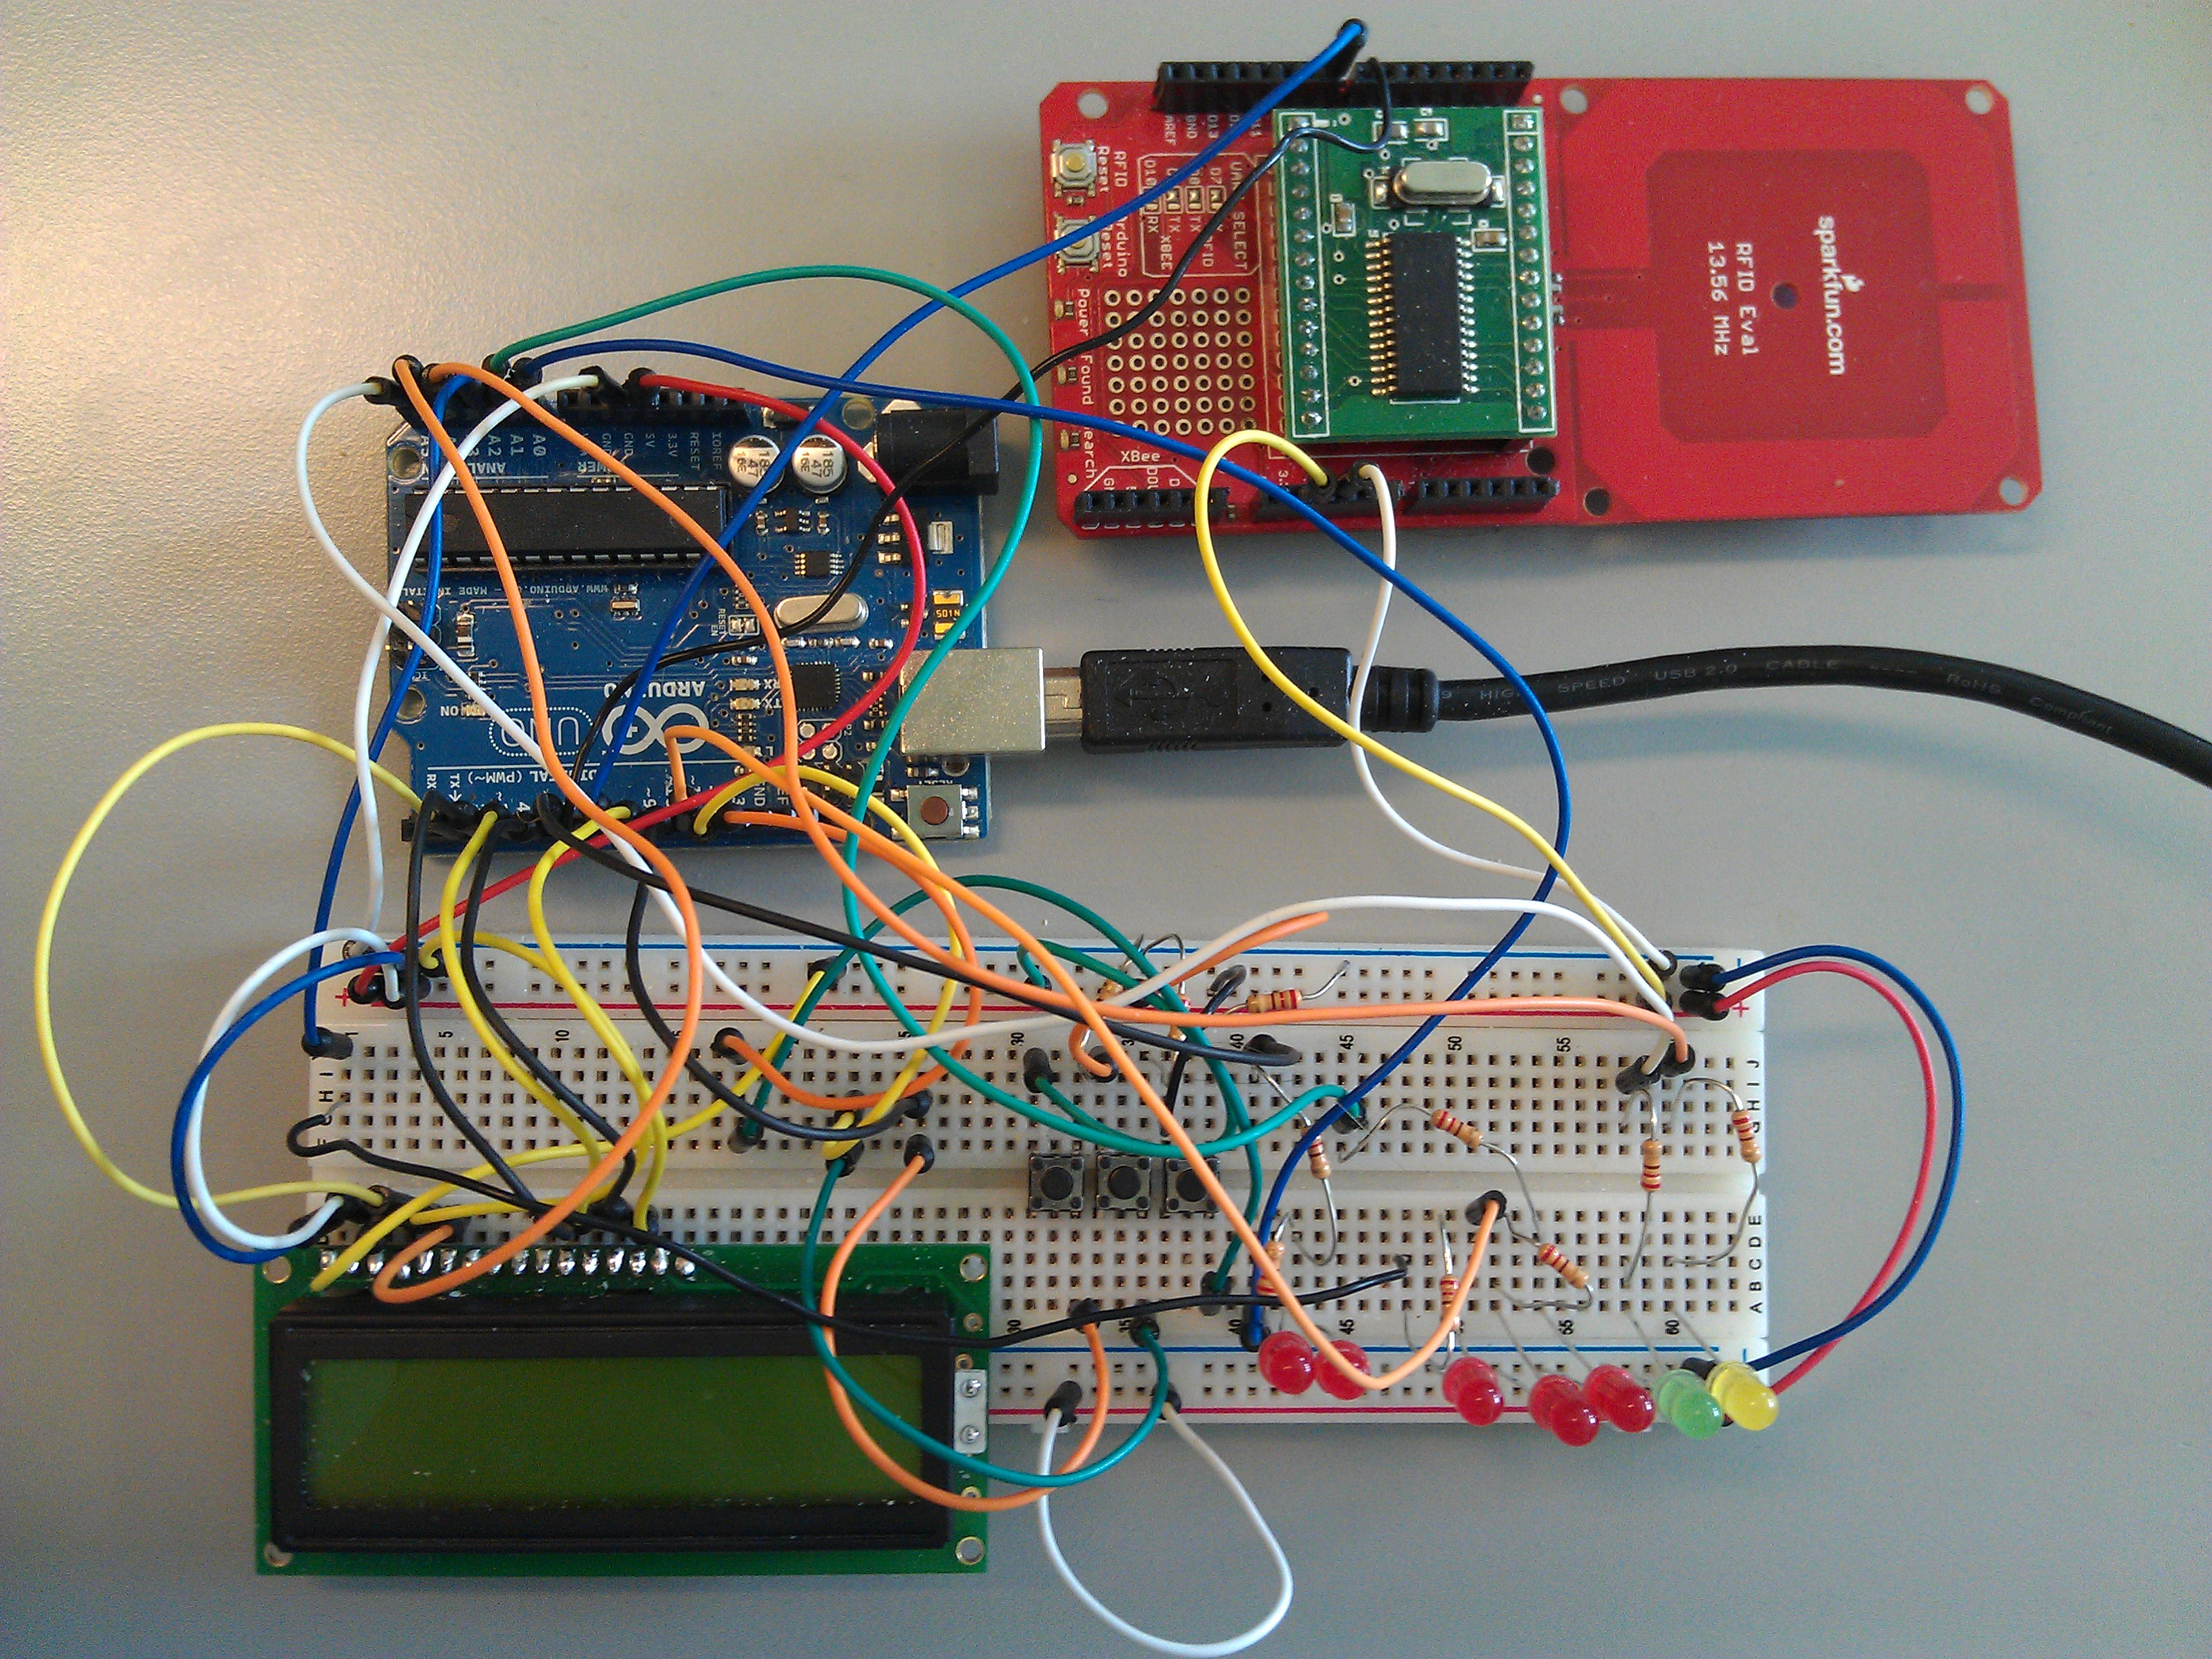
\includegraphics[width=0.8\textwidth]{billeder/HardwareSetup.png}

\vspace{1.5cm} 
\textsc{\Large SPLAD \\
P4 projekt\\
Group SW407F13\\
Software\\
Department of Computer Science\\
Aalborg University\\
May 2013\\
~\\
}

\includegraphics[width=0.35\textwidth]{billeder/AAUUKSTUDENTREPORTbluergb.png}
\end{flushright}

\cleardoublepage % Indsætter tom side (hvis nødvendigt)

% Dette er LaTeX-versionen af titelbladet for tek-nat-basis-rapporter 2004 efterår
% Filen kræver:
% Universitetets logo:  aau-logo.png (for LaTeX) eller aau-logo.ps (for LaTeX)
% Synopsis: En fil ved navn synopsis.tex

% Udarbejdet af: Hans Hüttel (hans@cs.auc.dk) 21. maj 2003
% Rettet af Morten Christophersen (mortench@tnb.aau.dk) 30. nov 2004(ændret til nyt design 2004 efterår)

%\documentclass[11pt]{article}
%\ifx\pdfoutput\undefined 
%\usepackage[dvips]{graphicx}
%\else
%\usepackage[pdftex]{graphicx} 
%\usepackage{type1cm} \fi
  %  \usepackage[ansinew]{inputenc}
    %\usepackage{a4}

%\begin{document} 
%\thispagestyle{empty}
%\begin{titlepage}

\begin{nopagebreak}
{\samepage
\hspace{8cm}
\begin{tabular}{r}
\parbox{\textwidth}{  \raisebox{11mm}{ 
\includegraphics[height=4cm]{billeder/AAUUKSTUDENTREPORTbluergb.png}}
\hfill
\\
\parbox{8cm}{\begin{tabular}{l}
{\small \textbf{Department of Computer Science}}\\
{\small Selma Lagerlöfs Vej 300} \\
{\small DK-9220 Aalborg East} \\
{\small http://www.cs.aau.dk/en}
\end{tabular}}}

\end{tabular}
\hspace{0cm}

\vspace{-5cm}
\begin{tabular}{cc}
\parbox{7cm}{
\begin{description}

\item {Titel:} 

SPLAT - Special Programming Language for Arduino Tipple-mixer

\end{description}

\parbox{8cm}{

\begin{description}
\item {Project period:}\\
   P4, spring 2012\\
  \hspace{4cm}
\item { Project group:}\\
  SW407F13\\
  \hspace{4cm}
\item { Group members:}\\
Aleksander Sørensen Nilsson \\
Christian Jødal O'Keeffe \\
Kasper Plejdrup\\
Mette Thomsen Pedersen \\
Niels Brøndum Pedersen \\
Rasmus Fischer Gadensgaard \\
  \hspace{2cm}
\item { Supervisor:}\\
Ricardo Gomes Lage\\
\end{description}
}
\begin{description}
\item { Total number of pages: }\\ \totalpages
\item { Project end: }\\
$29^{\text{th}}$ of May, 2013
\end{description}

\vfill } &
\parbox{7cm}{
  \vspace{.15cm}
  \hfill \\ \\
  \begin{tabular}{l}
  { Synopsis:}\\%\bigskip 
  \fbox{
    \parbox{6.5cm}{\bigskip
     {\vfill{\small This report starts off with a description of an environment where drinks are an essential part, this leads to the following problem statement:
"How can a programming language be developed, which makes it suitable for the hobbyist programmer to program drinks machines based on Arduino platforms?"
The product of this project is a programming language with a compiler which can make it easier to program a machine which can mix and serve drinks. The syntax of the program language is written in BNF and the compiler is developed using the parser and lexer generator ANTLR. Lastly, unit testing is used to test certain parts of the compiler to see if they work as intended. It has been concluded that this project gives a fulfilling answer to the problem stated in this project.
     \bigskip}}
     }}
   \end{tabular}}
\end{tabular}}
\\ \\


\noindent{\footnotesize\emph{The content of the report is freely available, but can only be published (with source reference) with an agreement with the authors.}}
\end{nopagebreak}
\vspace{0cm}
%\end{titlepage}
%\end{document}

\cleardoublepage
Dato:\indent\indent Aleksander Sørensen Nilsson\\\\\\
\indent\line(1,0){200}\\\\\\
\indent Dato:\indent\indent Christian Jødal O'Keeffe\\\\\\
\indent\line(1,0){200}\\\\\\
\indent Dato:\indent\indent  Kasper Plejdrup\\\\\\
\indent\line(1,0){200}\\\\\\
\indent Dato:\indent\indent  Mette Thomsen Pedersen\\\\\\
\indent\line(1,0){200}\\\\\\
\indent Dato:\indent\indent  Niels Brøndum Pedersen\\\\\\
\indent\line(1,0){200}\\\\\\
\indent Dato:\indent\indent  Rasmus Fischer Gadensgaard\\\\\\
\indent\line(1,0){200}\\\\\\

\cleardoublepage
\chapter{Prolog}
This report is written by Aleksander S. Nilsson, Christian J. O'Keeffe, Kasper Plejdrup, Niels  B. Pedersen, Mette T. Pedersen and Rasmus F. Gadensgaard as a 4th semester software project. We are a group of students from the Department of Computer Science at Aalborg University (AAU). This report documents and describes the process of designing and implementing a compiler.

The references in the report will be in the format [Example, year] with a corresponding entry in the bibliography in the back of the report just before the appendix. Figures and tables will be referred to in this manner: Table 3.5, where the first number is the chapter and the second number is the index of the figure or table in that chapter.

The DVD included on the last page of the report, see appendix \ref{chap:appDVD} contains the complete source code of the compiler, a PDF of the rapport, the compiled compiler and a sample program.

\cleardoublepage

%%%% Indholdsfortegnelse (TOC) %%%%


\setlength\parskip{0ex} % Fjerner den vertikale afstand mellem hver linie i indholdsfortegnelse
\tableofcontents* % Indholdsfortegnelsen 
\setlength{\parskip}{3mm} % Aktiverer afstanden igen for resten af rapporten (afstem med preamble!)

%\addtocontents{toc}{\protect\newpage} % Fremtvinger sideskift i indholdsfortegnelsen hvis nødvendig


\label{marker}
\mainmatter

 % Hovedindhold - nummereres fra side 1
\makeevenfoot{custom}{Side \thepage~af \pageref{LastPage}}{}{}	% Definerer lige siders sidefod efter modellen \makeevenfoot{Navn}{Venstre}{Center}{Højre}
\makeoddfoot{custom}{}{}{Side \thepage~af \pageref{LastPage}}% Definerer ulige siders sidefod efter modellen \makeoddfoot{Navn}{Venstre}{Center}{Højre}		
\pagestyle{custom}

\part{Udviklingsrapport}
%%%% Rapportindhold %%%%
\chapter{Indledning} 
Dette projekt fokuserer på at analysere et senarie i virkeligheden, som ifølge den objektorienterede arbejdsmetode kaldes problemområdet og få oprettet et objekt orienteret billede af problemområdet. Konflikterne i dette område skal derefter analyseres. Dette fører til en definition af anvendelsesområdet, hvor mulige aktører og brugsmønstre bliver fundet. Arbejdet leder så til, at det er muligt at designe et systemet, der skal fungere som en løsning på konflikterne i problemområdet.
Gruppen har valgt at anvende den iterative model frem for vandfalds-modellen. Den objektorienterede arbejdsmetode er beskrevet i \citep{ooaogd}.
Den iterative metode betyder, at alle disse aktiviteter foregår sideløbende med hinanden og i flere omgange.

I dette projekt har gruppen besluttet at arbejde med kundens handlen og den indbyrdes håndteringen af indkøbslister mellem kunderne.

\chapter{Problemanalyse}
\label{chap:problem}
I dette kapitel vil problemet blive analyseret. Problemområdet og anvendelsesområdet vil blive beskrevet. Ved hjælp af klassediagrammer og tilstandsdiagrammer vil problemområdet og anvendelsesområdet blive undersøgt. Analysen fungerer som udgangspunkt for designkapitlet, se kapitel \ref{chap:design}.

\section{Opgaven}
I denne sektion vil formålet med projektet blive beskrevet. Systemdefinition og omgivelserne vil desuden blive beskrevet. Med omgivelser menes problemområdet og anvendelsesområdet for dette projekt.

\subsection{Formål}
Det kan være vanskeligt og tidskrævende at overskue alle de ugentlige tilbud i dagligvarebutikker. Samtidig kan det også være svært at koordinere fælles indkøb mellem eksempelvis bofæller. Derudover er det praktisk hele tiden at have sin indkøbsliste på sig, da der kan opstå situationer, hvor man kunne bruge sin indkøbsliste. Derfor vil det være praktisk med et mobilbaseret indkøbslistesystem, der både kan finde de bedste tilbud ud fra en liste med indkøb, administrere indkøbslister, og som kan synkronisere mellem flere forskellige enheder. 

\subsection{Systemdefinition}
Systemet skal bruges til at administrere og finde tilbud på varer på en indkøbsliste. Systemet skal primært være et indkøbslisteprogram med tilbudsfunktion, som viser de bedste tilbud på de varer der står på indkøbslisten, men sekundært, skal det kunne foreslå tilbud, ud fra brugernes indkøbsvaner.  Systemet skal baseres på en mobil-optimeret hjemmeside, således at løsningen vil virke på gængse mobiloperativsystemer såsom Android, iOS og Windows Phone. Der skal i øvrigt tages hensyn til, at dele af systemet skal kunne betjenes med én hånd, da nogle områder af systemet typisk vil blive brugt i et supermarked, mens man handler. 

\begin{itemize}
\item \textbf{Betingelser:} Systemet skal fungere på forskellige platforme, og i forskellige hverdags-situationer.
\item \textbf{Anvendelsesområde:} Personer, par eller en gruppe, som køber ind, og er interesserede i at handle billigt.
\item \textbf{Teknologi:} Systemet skal være baseret på mobilenheder, således det kan bruges mens man handler.
\item \textbf{Objekter:} Kunder, indkøbslister, varer, tilbud og butikker.
\item \textbf{Funktionalitet:} Støtte til koordinering, administrering og tilbudssøgning.
\item \textbf{Filosofi:} Administrativt værktøj og indkøbsplanlægger.
\end{itemize}

\subsection{Omgivelser}
I dette afsnit gives et overblik over omgivelserne som repræsenterer problemområdet, dette vil blive beskrevet i detaljer i det næste afsnit \gaas{Problemområde}. Herunder på figur \ref{fig:RigtBillede} ses det rige billede, der er blevet lavet for at skabe overblik over problemområdet. 
\figur{1}{RigtBillede.png}{Rigt billede over problemområdet.}{fig:RigtBillede}

\subsubsection{Problemområde}
Problemområdet består af flere forskellige delproblemer, der vil blive set nærmere på. Et af delproblemerne er, at det kan være svært for par eller grupper, at koordinere indkøb indbyrdes, hvilket kan resultere i fejl i de foretagne indkøb. Dette delproblem bunder i kommunikationsproblemer mellem kunderne, som kan være resultatet af flere ting, bl.a. hvis de kommer til at tale forbi hinanden eller at en af kunderne misforstår den anden.


Et andet delproblem er, at det kan være besværligt for kunden, at få et overblik over alle de gældende tilbud på det tidspunkt, hvor indkøbslisten bliver skrevet. Med de mange forskellige tilbudsaviser kan det være tidskrævende og svært at skulle gennemse dem alle sammen, samt holde styr på de forskellige tilbud.

Det tredje delproblem er, at få delt indkøbslisten blandt de relevante personer. Hovedårsagen til dette ligger i papirformatet og det ekstra arbejde der ligger i at få fremstillet en kopi af indkøbslisten, dog findes der også løsninger, der tilbyder et elektronisk format af indkøbslister.

Disse tre delproblemer udgør tilsammen den del af problemområdet, som er i fokus i dette projekt.


\subsubsection{Anvendelsesområde}
Systemet skal lade kunder oprette sig som brugere. Systemet skal administrere brugertilgangen og derved tillade adgang til den pågældende kundes indkøbslister og programmets øvrige funktioner.
Gennem systemet skal kunderne kunne oprette indkøbslister, som kunden kan associere med andre kunder og derved dele den givne indkøbsliste indbyrdes.

Der skal være mulighed for at kunderne kan redigere deres tilknyttede indkøbslisters indhold, som systemet derefter skal gemme. Brugergrænsefladen skal bestå af de nødvendige elementer som gør det muligt for kunderne at tilgå de nødvendige funktioner de skal bruge i deres handlen.

Systemet skal også analysere kundernes indkøbslister og ud fra hvilke varer der er blevet købt, foreslå tilbud der kunne falde i kundens interesse. Til håndtering af tilbud skal systemet hente de informationer, der er nødvendige for, at kunden kan søge i tilbudene og tilføre de ønskede tilbud til den pågældende kundes indkøbsliste.
\section{Problemområdet}
I denne sektion vil der blive set nærmere på problemområdet for dette projekt, fra en objektorienteret vinkel. Til at få et indblik i problemet bliver der udviklet et diagram, et så kaldt klassediagram. Et klassediagram anvender UML (Unified Modeling Language) notation og bruges til at illustrerer de forskellige relationer mellem de forskellige klasser i problemområdet. Klasserne beskriver objekter ved, at fungere som skabelon for grupper af objekter, der har fælles træk. Klassediagrammet er bleven fremstillet ud fra viden fra OOAD (Objektorienteret analyse og design) bogen \citep{ooaogd} og selve diagrammet kan ses på figur \ref{fig:Klassediagram}.

\begin{landscape}
\figur{1.3}{AnalyseKlassediagram.png}{Oversigt over Klassediagram.}{fig:Klassediagram}
\end{landscape}

\subsection{Struktur}
For at få en bedre forståelse af strukturen i klassediagrammet på figur \ref{fig:Klassediagram} vil dette afsnit behandle de forskellige strukturer i klassediagrammet og beskrive dem.

\subsubsection{Klassen Kunde}
Klassen \gaas{Kunde} er en abstraktion af kunder fra den virkelige verden der handler ind, som enten kan være et medlem eller ikke-medlem af et selskab, derfor er klassen \gaas{Medlemskab} associeret med klassen \gaas{Kunde}.

Til klassen \gaas{Kunde} er klassen \gaas{Indkøbsliste} associeret, da en kunde kan have nul til mange indkøbslister. En indkøbsliste skal dog altid tilhøre mindst én kunde før den bliver relevant, da en indkøbsliste uden en kunde tilknyttet, vil betyde, at den ikke indeholder nogle varer der skal huskes.
Klassen \gaas{Kunde} er associeret med klassen \gaas{Begivenhed}. Grunden til associationen mellem klassen \gaas{Kunde} og \gaas{Begivenhed} er, at en person kan oprette nul til mange begivenheder og en begivenhed kan have en til flere personer tilknyttet angående arrangeringen af begivenheden.

\subsubsection{Klassen Indkøbsliste}
\gaas{Indkøbsliste} klassen udgør en væsentlig del af problemområdet og illustrerer netop den fysiske indkøbsliste, som der kan være problemer med at få delt og koordineret mellem de relevante kunder.

\subsubsection{Klassen Begivenhed}
Klassen \gaas{Begivenhed} er en abstraktion af alle de forskellige arrangementer en kunde kunne være interesseret i at oprette. Denne klasse er taget med fordi en kunde kan være interesseret i at oprette en indkøbsliste specifikt til et bestemt arrangement. Dette er grunden til at klassen \gaas{Indkøbsliste} er associeret til \gaas{Begivenhed} klassen.

\subsubsection{Klassen Medlemskab}
Klassen \gaas{Medlemskab} er associeret til \gaas{Selskab} i et forhold 1. Grunden til forholdet er, at et selskab ikke behøves at have nogle medlemmer men samtidig kan have flere end et medlem og der kan kun være ét selskab tilknyttet til en type medlemskab. 
En kunde kan også have flere medlemskaber af forskellige selskaber.

\subsubsection{Klassen Vare}
Den abstrakte klasse \gaas{Vare} er en abstraktion over de forskellige elementer en kunde kunne tilføje til deres indkøbslister. Denne abstraktion generaliseres til to underklasser \gaas{Almindelige Vare} og \gaas{Tilbud}. 

\gaas{Vare}-klassen bliver associeret med \gaas{Indkøbsliste}, således at der i modellen bliver dannet en relation mellem vare og indkøbsliste. Denne relation dækker over at en indkøbsliste indeholder nul til flere objekter af \gaas{Vare}, mens der stadig kan eksistere varer selvom de ikke er tilknyttet en indkøbsliste. Dette gør det muligt for varer at optræde på flere kunders indkøbslister samtidigt.

\gaas{Vare}-klassen bliver også associeret med \gaas{Tilbudsavis}, så der også bliver dannet en relation mellem vare og tilbudsavisen. Denne relation går ud på, at en tilbudsavis indeholder en til mange varer og et vareobjekt kun er tilknyttet én tilbudsavis af gangen. Dette gør at tilbud kun optræder én gang i en given tilbudsavis og at ét selskabs tilbud ikke fremkommer i et andet selskabs tilbudsavis.

\subsubsection{Klassen Tilbud}
\gaas{Tilbud} generaliseres derimod ud i endnu fire underklasser: \gaas{Pakketilbud}, \gaas{Mængdetilbud}, \gaas{Enkelttilbud} og \gaas{Medlemstilbud}. Dette er gjort, fordi der findes forskellige tilbud og alle disse skal håndteres i modellen. 

Klassen \gaas{Almindelig vare} er aggregeret til \gaas{Pakketilbud}, således at \gaas{Pakketilbud} består af to til flere \gaas{Almindelig vare}. Dette er gjort fordi pakketilbud består af flere almindelige varer, som i en kombination udløser rabatten. \gaas{Mængdetilbud} og \gaas{Tilbud} er med i modellen, for at kunderne kan anvende disse typer af tilbud. \gaas{Medlemstilbud} klassen er tilbud, som kun gælder for medlemmer af den specifikke butik, derfor har den attributten \gaas{betingelser}.

\subsubsection{Klassen Tilbudsavis}
For at sikre at kunderne i denne model kan anskaffe sig informationer om butikkernes tilbud, er der oprettet en klasse \gaas{Tilbudsavis}. \gaas{Tilbudsavis} er associeret med \gaas{Vare} i et forhold, der beskriver, hvordan en tilbudsavis kan have flere varer. \gaas{Tilbudsavis} er også associeret med \gaas{Selskaber} i forholdet en til mange, for at illustrere, hvordan forskellige butikskæder i samme selskab har deres udgave af tilbudsavisen ude på markedet, på samme tid.

\subsubsection{Klassen Selskab}
For at kunne håndtere de forskellige butikker og deres forskellige tilbud, er der blevet genereret en klasse \gaas{Selskab}, som abstraherer over dette område. Selskaber har så underklasserne \gaas{Butikskæder} og \gaas{Selvstændig butik}, hvor den selvstændige butik forstås som en privatejet butik.
Til \gaas{Butikskæder} er der aggregeret en \gaas{Butik}-klasse på, i et forhold, som fortæller, hvordan en butikskæde kan indeholde flere butikker. \gaas{Butik}-klassen illustrerer de individuelle butikker i en butikskæde.

\subsection{Klasser}
I denne sektion vil de forskellige klasser, samt deres tilstandsdiagram kort blive beskrevet.

\subsubsection{Kunde}
\figur{0.75}{AnalyseKundeTilstandsdiagram.PNG}{Viser tilstandsdiagrammet for klassen \gaas{Kunde}.}{fig:Kunde-tilstandsdiagram}
Klassen indeholder oplysninger om kunderne, således der er en måde at identificere kunder og kæde dem sammen med hinanden. Se figur \ref{fig:Kunde-tilstandsdiagram}.

Attributter: Navn, Forhold.

\subsubsection{Medlemskab}
\figur{0.75}{AnalyseMedlemTilstandsdiagram.PNG}{Viser tilstandsdiagrammet for klassen \gaas{Medlemskab}.}{fig:Medlem-tilstandsdiagram}
Klasse der beskriver en kundes mulighed for at have et medlemskab i et selskab, der så udløser en rabat, forskellige goder eller en form for præmie. Se figur \ref{fig:Medlem-tilstandsdiagram}.

Attributter: Rabat, Medlems ID.

\subsubsection{Indkøbsliste}
\figur{0.75}{AnalyseListeTilstandsdiagram.PNG}{Viser tilstandsdiagrammet for klassen \gaas{Indkøbsliste}.}{fig:Liste-tilstandsdiagram}
Klassen omfatter selve indkøbslisten, som er en liste af varer som kunden skal handle ind. Se figur \ref{fig:Liste-tilstandsdiagram}.

Attributter: Kunde.

\subsubsection{Begivenhed}
\figur{0.75}{AnalyseBegivenhedTilstandsdiagram.PNG}{Viser tilstandsdiagrammet for klassen \gaas{Begivenhed}.}{fig:Begivenhed-tilstandsdiagram}
Klassen der beskriver et scenarie, hvor kunden kan oprette en indkøbsliste i anledning af en begivenhed. Se figur \ref{fig:Begivenhed-tilstandsdiagram}.

Attributter: Tidspunkt, Navn.

\subsubsection{Vare}
\figur{0.75}{AnalyseVareTilstandsdiagram.PNG}{Viser tilstandsdiagrammet for klassen \gaas{Vare}.}{fig:Vare-tilstandsdiagram}
På figur \ref{fig:Vare-tilstandsdiagram} ses tilstandsdiagrammet for klassen \gaas{Vare}-Klassen sammenfatter de forskellige typer af varer. Her menes enten tilbud eller almindelige varer, her forstås almindelige varer som varer hvor der til normalpris. Tilbud indeholder fire generaliseringer, som bliver beskrevet i tilstandsdiagrammet for tilbud som set på figur \ref{fig:Tilbud-tilstandsdiagram}.
 
Attributter: Navn, Antal, mængdepris, pris.

\subsubsection{Tilbud}
\figur{1}{AnalyseTilbudTilstandsdiagram.PNG}{Viser tilstandsdiagrammet for klassen \gaas{Tilbud}.}{fig:Tilbud-tilstandsdiagram}
Denne klasse sammenfatter de forskellige slags tilbud som eksisterer. Se figur \ref{fig:Tilbud-tilstandsdiagram}. Disse klasser er beskrevet i klassediagrammet der kan ses på figur \ref{fig:Klassediagram}.

Attributter: Butik, Start dato, Slut dato.


%skal umildbart ikke tages med
%\subsection{Pakke tilbud}
%Klasse for gruppe af forskellige almindelige vare som til sammen udløser en rabat.

%Attributter:

%\subsection{Mængde tilbud}
%Klassen for mængde køb af en vare som udløser en rabat.

%Attributter: Min antal, Max antal per kunde.

%\subsection{Enkelt tilbud}
%Klasse for et almindeligt tilbud, hvor nuværende pris er mindre end før prisen.

%Attributter: 

\subsubsection{Selskab}
\figur{0.75}{AnalyseSelskabTilstandsdiagram.PNG}{Viser tilstandsdiagrammet for klassen \gaas{Selskab}.}{fig:Selskab-tilstandsdiagram}
Klasse for et selskab der kan eje forskellige butikskæder eller være en sammenslutning for private butiksejere. Se figur \ref{fig:Selskab-tilstandsdiagram}.

Attributter: Navn.

%Virker heller ikke til at skulle bruges
%\subsection{Kæde}
%Klasse for sammenfatningen af forskellige butikker af samme butikskæde, der eksister på markedet. Attributten antal beskriver antallet af butikker i den %individuel kæder.

%Attributter: Antal.

%\subsection{Butik}
%Klasse for de individuelle butikker der kan findes i en butikskæde.

%Attributter: Navn, Placering.

%\subsection{Enkelt butik}
%Klasse der beskriver de private butikker som ikke tilhøre en butikskæde.

%Attributter: Placering.

\subsection{Hændelser}

Tabel \ref{tab:haendelsestabel} viser en oversigt over hændelserne for de mest essentielle klasser. Ikke alle klasserne fra klassediagrammet (se figur \ref{fig:Klassediagram}) er taget med fordi de enten kan indgå som en underklasse eller som ses mindre væsentlige.

\begin{table}[H]
\centering
    \begin{tabular}{|l|c|c|c|c|}
\hline
        ~                                  & Vare & Kunde & Indkøbsliste & Selskab \\ \hline
        Indkøbsliste oprettet              & ~    & x     & x            & ~       \\ \hline 
        Indkøbsliste slettet               & ~    & x     & x            & ~       \\ \hline
        Indkøbsliste delt med andre        & ~    & x     & x            & ~       \\ \hline
        Vare tilføjet / slettet fra liste  & x    & ~     & x            & ~       \\ \hline
        Tilbud søgt                        & x    & ~     & ~            & x       \\ \hline
        Mulige butikker til indkøb valgt   &  ~   & x     & ~            & x       \\ \hline
        Begivenhed planlagt                & ~    & x     & x            & ~       \\ \hline
        Indkøbsliste tilknyttet begivenhed & ~    & ~     & x            & ~       \\ \hline
        Medlemskab af selskab startet      & ~    & x     & ~            & x       \\ \hline
        Medlemskab af selskab sluttet      & ~    & x     & ~            & x       \\ \hline
        Tilbud oprettet                    & x    & ~     & ~            & x       \\ \hline
        Tilbud afsluttet                   & x    & ~     & ~            & x       \\ \hline 
        Tilbuds-avis udsendt               & ~    & x     & ~            & x       \\ \hline
        Ny butik åbnet                     & ~    & ~     & ~            & x       \\ \hline
        Butik lukket                       & ~    & ~     & ~            & x       \\ \hline
        Vare købt                          & x    & ~     & x            & ~       \\
\hline
    \end{tabular}

\caption{Tabel for de forskellige hændelser tilhørende de mest essentielle klasser som vare, kunde, indkøbsliste og selskab.}
\label{tab:haendelsestabel}
\end{table}

\section{Anvendelsesområde}
Dette afsnit vil omhandle anvendelsesområdet, hvor der vil blive set nærmere på aktørerne og brugsmønstrene. Ud fra brugsmønstrene vil der blive lavet funktioner der vil håndtere brugsmønstrene og give den ønskede funktionalitet til systemet.
Brugergrænsefladen vil også blive gennemgået (se sektion \ref{sec:brugerflade}) og vist gennem nogle eksempler, der illustrerer en mulig brugergrænseflade for systemet.

\subsection{Brug}
For at opnå en bedre forståelse af, hvorledes systemet skal hjælpe kunderne, vil der blive set nærmere på aktørerne og deres brugsmønstre.

\subsubsection{Oversigt}
Der er blevet identificeret to aktører: En indkøber og en planlægger og i alt seks brugsmønstre, der involverer disse to aktører. Det kan dog godt være en person, som har begge aktørroller. Disse kan ses i tabel \ref{tab:Aktoertabel}.

\begin{table}[H]
\centering
    \begin{tabular}{|l|c|c|}
\hline
        ~                                       & Indkøberen & Planlæggeren  \\ \hline
        Tilføj til indkøbsliste                 & ~          & x             \\ \hline 
        Slet fra indkøbsliste                   & ~          & x             \\ \hline
        Markér vare                             & x          & ~             \\ \hline
        Del liste                               & ~          & x             \\ \hline
        Opret indkøbsliste                      & ~          & x             \\ \hline
        Slet indkøbsliste                       & ~          & x             \\ \hline
        Find tilbud                             & ~          & x             \\ \hline
    \end{tabular}

\caption{Aktørtabellen over de fundne aktører samt deres brugsmønstre.}
\label{tab:Aktoertabel}
\end{table}

\subsubsection{Aktører}
\begin{table}[H]
    \begin{tabularx}{\textwidth}{R}
    	\hline
        \textbf{Indkøberen} \\ \hline
        \textbf{Formål:} Er en person som handler ind ud fra en indkøbsliste. \\
        \textbf{Karakteristik:} Arbejdet udføres af personer med varierende teknologisk erfaring.   \\
        \textbf{Eksempler:} Økonomisk bevidst forbruger, som lever på et stramt budget, besidder en 
        basal teknologisk erfaring og har en smartphone.\\
        Et ungt par med begrænsede midler, middel teknologisk erfaring, begge har en smartphone.
    \end{tabularx}
\end{table}

\begin{table}[H]
    \begin{tabularx}{\textwidth}{R}
    	\hline
        \textbf{Planlæggeren} \\ \hline
        \textbf{Formål:} En person, som benytter en indkøbsliste til at planlægge sine daglige indkøb ved hjælp af en indkøbsliste,
        og som samtidig interesserer sig for at købe sine dagligvarer billigst muligt.\\
        \textbf{Karakteristik:} Arbejdet udføres af personer med varierende teknologisk erfaring og med sans for overblik. \\
        \textbf{Eksempler:} Økonomisk bevidst forbruger, som lever på et stramt budget, besidder en basal teknologisk erfaring og har en smartphone.\\
        Et ungt par med begrænsede midler, middel teknologisk erfaring og begge har en smartphone.
    \end{tabularx}
\end{table}

\subsubsection{Brugsmønstre}

De syv brugsmønstre kan kategoriseres i grupperne \gaas{Administrering af varer på indkøbslisten}, \gaas{Administrering af indkøbslisterne} og \gaas{Find tilbud}.

\textbf{Administrering af varer på indkøbslisten}

\begin{itemize}
	\item Tilføj til indkøbsliste
	\item Slet fra indkøbsliste
	\item Markér vare 
\end{itemize}

Mønster: En aktør ønsker at indsætte en vare på en indkøbsliste, og derfor skal systemet kunne håndtere dette. Desuden vil aktøren gerne kunne slette varer fra indkøbslisten igen, når de er købt. En aktør skal kunne markere de varer han/hun har lagt i indkøbsvognen, således at aktøren er klar over, hvilke varer han/hun mangler at finde. Derfor skal der være en funktion i systemet, der kan holde styr på, hvad aktøren har \gaas{købt} på det bestemte tidspunkt.

\textbf{Administrering af indkøbslisterne}

\begin{itemize}
	\item Del liste
	\item Opret indkøbsliste
	\item Slet indkøbsliste
\end{itemize}

Mønster: Det skal være muligt for en aktør at kunne oprette en indkøbsliste og tilføje varer og tilbud til denne. Desuden skal det være muligt at slette indkøbslisten igen når den har tjent sit formål. Hvis en aktør ønsker at dele en indkøbsliste med en anden aktør, skal systemet kunne håndtere flere aktører der deles om en indkøbsliste. Således en vare eller tilbud ikke bliver købt flere gange af de forskellige aktører der deler indkøbslisten.

\textbf{Find tilbud}

\begin{itemize}
	\item Find tilbud
\end{itemize}

Mønster: Det skal være muligt for aktører at bruge systemet til at finde tilbud. Altså skal der være en funktion til at søge efter tilbud i løsningen.

\subsection{Funktioner}
De nødvendige funktioner for systemet der skal udvikles i dette projekt kan ses på tabel \ref{tab:funktionstabel}. Funktionerne er designet så de understøtter hændelserne angivet i problemområdet, som kan ses i tabel \ref{tab:haendelsestabel}.
\begin{table}[H]
\centering
    \begin{tabular}{|l|c|c|}
        \hline
    Funktioner                                          & Kompleksitet & Type        \\ \hline
	Find tilbud                                         & Medium       & Aflæsning   \\ \hline
	Opret indkøbsliste                                  & Simpel       & Opdatering  \\ \hline
	Knyt person til en indkøbsliste                     & Simpel       & Opdatering  \\ \hline
	Slet indkøbsliste                                   & Simpel       & Opdatering  \\ \hline
	Tilføj vare til indkøbsliste                        & Simpel       & Opdatering  \\ \hline
	Slet vare fra indkøbsliste                          & Simpel       & Opdatering  \\ \hline
	%Find ofte købte varer                               & Kompleks     & Beregning og aflæsning  \\ \hline
	%Find tilbud ud fra ofte købte varer                 & Medium       & Beregning   \\ \hline
	Foreslå tilbud                                      & Kompleks     & Signal, Beregning og aflæsning    \\ \hline
    \end{tabular}
\caption{Tabel over funktioner baseret på hændelsestabellen.}
\label{tab:funktionstabel}

\end{table}
På tabel \ref{tab:funktionstabel} kan det ses, at der for systemet findes en række simple funktioner. Derudover findes der en kompleks funktion samt en medium. \gaas{Find tilbud}-funktionen inkluderer at finde et tilbud til kunden, ud fra nogle givne kriterier som fx en søgestreng. Funktionen der er en aflæsnings-funktion, skal have en kilde med tilbud den kan aflæse. For at finde fremtidige tilbud skal systemet kunne foreslå tilbud til kunden ud fra tidligere køb. Dette er en kompleks funktion, fordi en person der bruger et sådan system naturligt vil skrive sine indkøb på mange forskellige måder, samt tilføje tilbud med forskellige titler. Denne komplekse funktion \gaas{Foreslå tilbud} skal altså gå igennem kundens indkøbslister og finde de varer der ofte bliver købt. Derefter vil funktionen ud fra resultaterne søge efter tilbud og vise forslagene til kunden.

\subsection{Brugergrænsefladen}
\label{sec:brugerflade}
I dette afsnit vil dialogformen blive beskrevet. Der vil desuden blive vist skitser af brugergrænsefladen, og tanken bag disse vil blive beskrevet.
\subsubsection{Dialogform}
For at aktørerne kan navigere rundt er der blevet lavet en menu der gør navigationen nemmere. Når aktører kommer med input vil der enten være en tekstboks eller en knap således at aktøren klart kan se formålet med inputtet og hvad systemet skal bruge inputtet til.
%Hvis aktøren skulle bruge kommandosprog, ville det tage lang blive lære at bruge systemet og det kunne være vanskelig hele tiden at skrive kommandoer mens man køber ind. Især på en mobilenhed hvor man som regel ikke har et keyboard til at taste ind med.
Brugergrænsefladen vil have et vindue med søgefunktionen, indkøbslisterne og de tilbud, som systemet foreslår ud fra brugerens indkøbsvaner. Ud over dem, vil der være indstillinger, hvor aktøren vil kunne indstille forskellige indstillinger ved systemet, såsom hvilke butikker aktøren vil have tilbud fra. Nedenstående liste viser en oversigt over de forskellige vinduer.

\begin{itemize}
	\item Hovedvindue
	\item Log ind
	\item Søge-funktion
	\item Indkøbslister
	\item Foreslåede tilbud
	\item Indstillinger
\end{itemize}

%Vi vælger en store menu-knapper til at navigere rundt på siden, og skemaudfyldelse til indtastning af data. Brugerne kan direkte manipulere dele af hjemmesiden, såsom at krydse elementer på indkøbslisten af. 
%Har vi lavet så man kan scanne stregkoder? Så bør der nok stå noget om det her.. ;)
%Det ville ikke give mening at bruge kommandoer på en mobil-optimeret hjemmeside. Brugergrænsefladen har separate sider, som er forbundet af links på de individuelle sider. Således kan brugeren blive guidet til de relevante funktioner ud fra den side brugeren ser på nuværende tidspunkt.

\subsubsection{Oversigt}
\figur{1.0}{AnalyseOversigtOverGUI.png}{Diagram over strukturen mellem de forskellige vinduer.}{fig:OversigtOverGUI} %billede nu sat ind men det skal huskes at billede også skal rettes
På figur \ref{fig:OversigtOverGUI} kan der ses et navigerings-diagram, der giver et overblik over, hvordan aktører kommer rundt i systemet. Vinduerne er baseret på skabelonerne og giver en generel idé om hvordan løsningen kommer til at %er det det rigtige ord? 
se ud på en mobilenhed. %Alle funktionerne i systemet som aktøren kan bruge bliver vist i vinduerne, hvilket gør at der skabes et vist overblik over systemet. 

\subsubsection{Eksempler}
Der er blevet lavet nogle skabeloner for at give et generelt indblik i, hvorledes systemet grænsefladen mellem aktøren og systemet kan se ud.

\figur{0.4}{StartskaermEndelig.png}{Her ses en skitse over hvordan det var planlagt, startskærmen skulle se ud.}{fig:Startskaerm}
Figur \ref{fig:Startskaerm} viser startskærmen, som giver adgang til alle hjemmesidens andre funktioner. Via tryk på billederne var det meningen, at en bruger skulle sendes videre til den valgte funktion, og ved at trykke på \gaas{log ind}-knappen skulle det være muligt at logge ind.

\figur{0.4}{LogIndSkaermEndelig.png}{Her ses en skitse over, hvordan man skulle logge ind.}{fig:LogInd}
Figur \ref{fig:LogInd} viser, hvordan \gaas{Log ind}-boksen oprindeligt var designet.

\figur{0.4}{SoegeFunktionEndelig.png}{Her ses en skitse over, hvordan det var planlagt søgefunktionen skulle se ud.}{fig:Soegefunktion}
Figur \ref{fig:Soegefunktion} viser søgefunktionen, hvor brugeren ville have mulighed for at søge efter tilbud, og derefter kunne tilføje tilbuddet til en indkøbsliste.

\figur{0.4}{IndkoebslisteSorteretEfterButikker1Endelig.png}{Her ses en skitse over, hvordan udseendet til indkøbsliste blev tænkt, sorteret efter butikker.}{fig:ListeButikker}
Figur \ref{fig:ListeButikker} viser, hvordan indkøbslisten ville se ud hvis den var sorteret efter butikker først og varekategori derefter.

\figur{0.4}{IndkoebslisteSorteretEfterKategori2Endelig.png}{Her ses en skitse over hvordan indkøbslisten skulle se ud sorteret efter varekategori og derefter inddelt efter butikker.}{fig:ListeKategorier}
Figur \ref{fig:ListeKategorier} viser hvordan det oprindeligt var tænkt at indkøbslisten skulle se ud. Sorteret først efter kategori og derefter inddelt efter butik.

\figur{0.4}{ForslaaedeTilbudEndelig.png}{Her ses en skitse over, hvordan funktionen til at forslå tilbud, skulle se ud.}{fig:ForslaaedeTilbud}
Figur \ref{fig:ForslaaedeTilbud} viser funktionen til at foreslå tilbud. Funktionen skulle vise de tilbud en funktion havde analyseret sig frem til, som vil kunne interessere den enkelte bruger.

\subsection{Den tekniske platform}
Systemet skal udvikles som en webbaseret løsning, hovedsageligt tilpasset mobile enheder, men samtidig også tilgængeligt på en mere stationær enhed. Systemet skal programmeres i C\#, som også fungerer som et passende sprog i forhold til den objektorienteret model, der også er fortaget analyse ud fra. Systemet er rettet mod mobile enheder da det typisk vil være en sådan enhed, der vil blive benyttet mens man handler, frem for eksempelvis en bærbar computer.
Til systemet skal der bruges en database, hvor det er muligt at definere passende tabeller, således det er muligt at konstruere en relevant databasestruktur. Databasen skal også være tilgængelig for de eventuelle kommende brugere. 
Systemet skal opbygges efter almindelig hjemmesidestandarter og stadig være optimeret til mobile enheder.
Systemet skal betjenes via berøringsnavigation for de mobile enheder, og for de stationere enheder skal der bruges mus og tastetur.
Optimeringen rettet imod mobile enheder, skal sikre at systemet bliver mere brugervenligt angående berøringsnavigation. 
\section{Anbefalinger}
Dette afsnit handler om hvor realiserbart systemet er, og hvordan systemet vil blive implementeret.

\subsection{IT-systemets nytte og realiserbarhed}
Den beskrevne funktionalitet af systemet er blevet gennemgået for nogle potentielle brugere. Derudover er der blevet lavet en prototype af systemet med fokus på brugergrænsefladen. Systemet anses, på den baggrund, for at have et passende ambitionsniveau i forhold til hvad der er muligt.
Den tekniske erfaring i projektgruppen gør det muligt, uden alt for store problemer og inden for den angivne ramme, at implementere den i det forslåede udformning.

\subsection{Strategi}
Brugerne og systemudviklerne er begge enige om at det beskrevne system skal udvikles. Systemet forventes implementeret i C\# med ASP.NET da det er et webbaseret system. Tests vil blive udført sideløbende med at systemet bliver udviklet.

\section{Problemformulering}
\label{sec:problem}
I denne sektion vil hovedproblemet blive fremsat, hvorefter det vil blive delt op i delproblemer, som problemløsningen vil beskrive en løsning på, med udgangspunkt i analysedokumentet.
Ud fra analysedokumentet kommer hovedproblemet:

\textbf{Hvordan kan et IT-system laves, der kan hjælpe brugeren med at finde de bedste tilbud på de varer der er på en given indkøbsliste, hjælpe brugeren med at koordinere indkøb med andre brugere, samt finde tilbud af interesse ud fra brugerens indkøbsvaner?}

Det kan ses ud fra beskrivelsen af problemområdet og anvendelsesområdet, hvor IT-systemet skal kunne hente og registrere informationer. Informationen skal systemet kunne anvende på brugernes indkøbsliste, således at den finder de billigste varer i de udvalgte butikker.
Delproblemerne er lavet for at hjælpe med at finde løsningen til hovedproblemet.
\begin{itemize}

\item\textbf{Hvordan kan de forskellige klasser og hændelser håndteres i et IT-system?}

IT-systemet skal kunne arbejde med forskellige klasser og hændelser, som er fundet i analysedokumentet. Det er nødvendigt at finde ud af, hvordan systemet kan håndtere klasser og deres hændelser. 

\item\textbf{Hvad kan gøres for at opgaven med at at finde tilbud bliver nemmere og hurtigere?}

Løsningen skal gøre det nemmere og hurtigere at lave en indkøbsliste, ud fra tilbud den pågældende uge.

\item\textbf{Hvordan kan en brugers indkøb analyseres, således at der kan foreslås nye tilbud til brugeren?}

Løsningen skal ud fra brugernes indkøbsvaner foreslå relevante varer, som er på tilbud den pågældende uge.

\item\textbf{Hvordan kan det gøres nemmere for en bruger at koordinere sine indkøb med en eller flere personer?}

Løsningen skal gøre det nemmere for en bruger at koordinere sine indkøb med andre, så brugeren ikke risikerer at ende op med dubletter af en given vare.

\end{itemize}
\section{Afrunding af problemanalyse}
I dette kapitel er der blevet set på, hvad problemområdet består af og hvilke problematikker, der skal behandles for at kunderne, de potentielle brugere, kan anvende systemet som en løsning på de opstillede problematikker. Der kommer en generalisering af problemområdet, for at få et overblik over, hvad anvendelsesområdet skal være i stand til at kunne.

Et værktøj der blev brugt til at danne overblik over problemområdet, er det rige billede som ses på figur \ref{fig:RigtBillede}, som bruges til at illustrere problemområdet og de konklifter, der kan findes i problemområdet. Gennem analysen af problemområdet, er det blevet gjort klart, at problemet består af tre delproblemer, der dækker over de forskellige konflikter, som kan opstå i problemområdet. Disse tre delproblemer er henholdsvis deling af indkøbslisterne, synkronisering mellem flere indkøbslister og til sidst håndteringen af tilbud i forhold til indkøbslister.

Et andet værktøj, som også blev brugt til at kortlægge problemområdet er et klassediagram, som indholder de forskellige klasser og deres relationer til hinanden, som de kan observeres i den virkelige verden, samt deres hændelser. Til klassediagrammet følger en forklaring af strukturen i klassediagrammet. Selve klasserne er også beskrevet samt deres tilstandsdiagrammer, der illustrerer hvorledes de forskellige klasser skifter tilstande.

Klassediagrammet bliver derefter brugt i arbejdet med anvendelsesområdet. Til arbejdet med anvendelsesområdet bliver der set nærmere på, hvilke redskaber der er egnet til udviklingen af systemet. Der bliver også defineret to aktører, samt brugsmønstre der fortæller om, hvordan disse aktører vil bruge systemet i den givne problemstilling. Ud fra brugsmønstrene er der blevet udviklet funktioner, der understøtter hændelsestabellen.

Til sidst er der blevet udviklet en problemformulering, som afspejler essensen af dette projekt. Det videre arbejde vil ligge i, at få designet de komponenter, som vil udgøre systemet, se på kvalitetsmålene for udviklingen og se nærmere på hvilken platform systemet skal fungere på.

\chapter{Design}
\label{chap:design}
I dette projekt er formålet at fremstille en løsning, som skal hjælpe brugerne med at ordne og koordinere indkøbene ordenligt mellem brugerne. Det vil sige at løsningen skal være tilgængelig for flere brugere og derved hjælpe brugerne med at kommunikere og koordinere deres indkøb på en let og brugervenlig måde.

I dette kapital vil der blive defineret en systemspecifikation, der skal bruges til, at udvikle et design for programmets forskellige komponenter. Disse komponenter vil derefter blive sat i en struktur, der til sidst vil udgøre en potentiel løsning på det givne problem. Der vil også blive beskrevet, hvordan grænsefladen mellem brugerne og programmet er, og hvordan den anvendes mest effektivt.
%Vedrørende den tekniske platform, det vil sige, platforme programmet kan bruges på, valg af designsprog og eventuelt andre tekniske begrænsninger. 
De forskellige relevante klasser ville blive specificeret samt sat i en struktur der senere kan anvendes i selve udviklingen af problemløsningen.

\section{Opgaven} %Kriterier for Produktet
%tjek op imod bogen, og det passer det der er skrevet. altså om de forskellige kriterier er beskrevet ud fra de de rent faktisk betyder.
I dette afsnit vil der blive set nærmere på de forskellige kvalitetsmål og hvordan de er prioriteret i dette projekt.
Prioriteringer vil blive illustreret i en tabel, hvorefter de individuelle prioriteringer vil blive beskrevet og begrundet.

\subsection{Formål}
Produktløsningen har til formål at hjælpe med koordineringen af indkøb, tilbudssøgning på varer og forslå varer der ofte bliver købt ved at analysere den pågældende kundes indkøbsvaner.
Gennem disse funktionaliteter skal produktløsningen hjælpe kunderne i deres handel og være et alternativ til en almindelige indkøbsliste eller andre løsninger.

\subsection{Rettelser til analysen}
\label{sec:rettelsertilanalyse}
Der er foretaget omfattende ændringer i klassediagrammet, se figur \ref{fig:Klassediagram}, fra analysedokumentet, da nogle af klasserne blev fundet trivielle for produktløsningen. Her er der tale om at ti ud af de femten klasser blev fundet ubetydelige for problemløsningen. De klasser der er taget med er \gaas{Kunde}, \gaas{Indkøbsliste}, \gaas{Vare}, \gaas{Tilbud} og \gaas{Butik}. De fravalgte klasser er blevet frasorteret, da der ikke skal tages specielt hensyn til disse i problemløsningen. De fem valgte klasser dækker alle de informationer, der vil blive nødvendige i problemløsningen.

\subsection{Kvalitetsmål}
\label{sec:kvalitetsmaal}
For at få en mere retningsbestemt udvikling, er der blevet specificeret og prioriteret nogle kvalitetsmål. Kvalitetsmålene fungerer som retningslinjer for hvilke områder, der vil blive fokuseret på og illustrerer hvilke områder, der er vigtige for systemet. Disse kvalitetsmål og deres prioriteringer indsættes i en tabel for at danne en sammenhæng mellem dem. Et overblik over, hvad der er prioriteret kan ses på tabel \ref{tab:kriterier}. Kvalitetsbogen er baseret på definitionerne i \citep{ooaogd}.

\begin{table}[H]
\centering
\begin{tabular}{|c | c | c | c | c | c | c|}
\hline
\textbf{Kvalitetsmålene} & \rotatebox{90}{Meget vigtigt} & \rotatebox{90}{Vigtigt} & \rotatebox{90}{Mindre vigtigt} & \rotatebox{90}{Irrelevant} & \rotatebox{90}{Trivielt opfyldt~}\\ \hline
Brugbart        & x &   &   &   &      \\ \hline
Forståeligt     & x &   &   &   &      \\ \hline
Pålideligt      &   & x &   &   &      \\ \hline
Effektivt       &   & x &   &   &      \\ \hline
Korrekt         &   & x &   &   &      \\ \hline
Testbart        &   & x &   &   &      \\ \hline
Vedligeholdbart &   &   & x &   &      \\ \hline
Flytbart        & x &   &   &   &      \\ \hline
Genbrugbart     &   &   &   & x &      \\ \hline
Sikkert         &   &   & x &   &      \\ \hline
Fleksibelt      &   &   & x &   &      \\ \hline
Integrerbart    &   &   &   & x &      \\ \hline

\end{tabular}
\caption{Denne tabel fungerer som en oversigt over, hvordan de forskellige kriterier er prioriteret i forhold til hinanden.}
\label{tab:kriterier}
\end{table}
\textbf{Brugbart:}
Systemet skal være brugbart, da brugerne anvender det i deres dagligdag. Heri ligger det, at systemet skal være let anvendelig både stående, gående eller siddende da brugerne befinder sig i en af disse tre tilstande, når de handler ind. Og da det skal bruges til en bred vifte af brugere, skal det være let og simpelt at bruge, så der ikke er for mange funktioner og lignende man skal sættes ind i. Dette vil sige at systemet skal være designet mod mobile enheder, da det er den platform der egner sig bedst til kundernes handel. Derfor er \gaas{brugbart} prioriteret \gaas{meget vigtigt}.

\textbf{Forståeligt:}
For at gøre det lettere for brugerne skal systemet også være let forståeligt. Dette gøres ved at gøre det overskueligt. Derfor er \gaas{forståeligt} også prioriteret \gaas{meget højt} ligesom \gaas{brugbart}.

\textbf{Pålideligt:}
Udover at systemet skal være brugbart, skal det også være pålideligt, da brugerne altid skal kunne stole på systemet. Hvis brugerne får givet forkerte oplysninger kan det lede til, at brugerne ikke får koordineret indkøbene efter hensigten, og derved mister problemløsningen et af sine primære formål. Det nytter heller ikke, at systemet tilføjer ting til indkøbslisten som ingen af brugerne har skrevet ind. Derfor er det vigtigt at systemet er pålideligt, da dette sikrer en meget bedre brugeroplevelse af problemløsningen. Det er naturligvis ikke muligt at sikre pålideligheden i alle situationer, eksempelvis kan brugerens internetforbindelse blive tabt. Der menes derfor at den del af systemet brugerne kan påvirke skal være pålideligt.

\textbf{Effektivt:}
Kvalitetsmålet \gaas{effektivt} betyder at problemløsningen skal fungere i en rimelig hastighed således brugeren ikke skal vente længe på, at problemløsningen henter eller sender data. Dette kvalitetsmål er sat til \gaas{vigtigt}, da systemet gerne skulle fungere så hurtigt som det nu engang er muligt for det givne system. Samtidig skal det udføre så få database-kald og API-kald som muligt, netop for at mindske ventetiden.

\textbf{Korrekt:}
Systemet skal også følge de mål, der er blevet sat i projektet så godt som muligt, så systemet rent faktisk opfylder de krav, der er blevet stillet. \gaas{Korrekt} er derfor prioriteret som værende \gaas{vigtigt}. Derudover skal der være konsistens i systemet, således at brugerne kan forvente at kunne navigere ensartet gennem hele systemet. 

\textbf{Testbart:}
Systemet skal være testbart, således at det er muligt at teste de forskellige kvalitetsmål og derved bedømme om den ønskede korrekthed er opnået. Dette prioriteres som \gaas{vigtigt} da det i forhold til \gaas{brugbart} eller \gaas{forståeligt} ikke ses lige så vigtigt, men det er lige så vigtigt som \gaas{effektivt} da det kan gøre systemet nemmere for brugeren at bruge.

\textbf{Vedligeholdbart:}
For at have mulighed for at vedligeholde systemet, skal systemet udvikles og udformes på en måde, der gør det nemmere at udskifte dele som ikke længere virker i sammenhæng med resten af systemet. Derfor er \gaas{vedligeholdbart} blevet prioriteret som værende mindre vigtigt, da systemets informationskilde ikke kommer til at ændre sig meget.

\textbf{Flytbart:}
\gaas{Flytbart} er prioriteret som \gaas{meget vigtigt}, idet det er vigtigt at løsningen kan fungere på forskellige enheder, da det er sandsynligt at eksempelvis par, som vil benytte løsningen sammen, ikke har ens enheder, eller at den enhed de bruger i hjemmet er en anden enhed, end den de tager med sig når de skal handle. Derfor bør løsningen fungere på forskellige platforme, og med forskellige browsere. 

\textbf{Genbrugbart:}
Det anses ikke for nødvendigt at systemet skal være \gaas{genbrugbart}. Derfor er dette kvalitetsmål også prioriteret som værende \gaas{irrelevant}.

\textbf{Sikkert:}
Systemet skal også i et vist omfang være sikkert for brugerne, da de bliver nødt til at logge ind i systemet for få adgang til deres indkøbslister og nogle bruger det samme kodeord på flere forskellige sider. Derfor er det blevet vurderet, at det er nødvendigt at have kryptering af \gaas{log ind} informationer. Dog er sikkerhed ikke fokuspunktet for dette system, idet systemet ikke behandler personfølsomme informationer. Grundet dette er sikkerhed blevet prioriteret som \gaas{mindre vigtigt} for dette system.

\textbf{Fleksibelt:}
For at sikre at systemet ikke går ned under brug, skal systemet være fleksibelt nok til at kunne håndtere forskellige fejl uden at gå ned. Derfor er \gaas{fleksibelt} kvalitetsmålet blevet prioriteret \gaas{mindre vigtigt} idet det ikke er ligeså vigtigt som de andre vigtige kvalitetsmål, men samtidig er relevant for det givne system.

\textbf{Integrerbart:}
Da systemet i dette projekt i denne omgang kun er tiltænkt integreret på webserveren, er integrerbart ikke vurderet til at være vigtigt, sammenlignet med de andre kriterier. Det er derfor vurderet til at være \gaas{irrelevant}.

%\input{eksisterendeloesninger.tex}

\section{Teknisk platform}
Her vil der blive beskrevet hvilket udstyr, basisprogrammeller systemgrænseflader og designsprog, som problemløsningen kommer til at involvere.

\subsection{Udstyr}
Mobile enheder er en god platform at arbejde ud fra, men de kan være besværlige at skrive længere indkøbslister på. Derfor kan det være funktionelt at få adgang til indkøbslisten fra andre mere stationære platforme, for eksempel en computer.

\subsection{Basisprogrammel}
For bedre at kunne udvikle et produkt der kan løse problemet, skal der bruges et programmeringssprog der egner sig til at arbejde med objekter, forbindelser mellem disse objekter og deres anvendelsesområder. Grunden til at der bliver arbejdet med objekter i dette projekt er, at det giver bedre mulighed for at abstrahere over problemområdet. Den objektorienterede struktur er med til at skabe sammenhæng og give et overskueligt billede af problemløsningen. Derfor vil produktet blive skrevet i C\# med ASP.NET framework, hvor Microsoft Visual Studio vil fungere som arbejdsplatform. C\# er valgt fordi det er et objektorienteret sprog og derfor passer til metoden, der bliver arbejdet ud fra i dette projekt.

\subsection{Systemgrænseflade}
Problemløsning vil komme til at fungere sammen med en hjemmeside, der ligger inde med en database over tilbud fra forskellige butikskæder. Arbejdet ligger i at kommunikere med databasen igennem en API og anvende de relevante informationer til at løse problemet. Problemløsningen vil også arbejde sammen med en brugerdatabase, for at kunne synkronisere med andre forbundne brugere, holde styr på hvilke indkøbslister der er tilknyttet hvilke brugere og hvilke varer, der står på hver enkelt indkøbsliste. 

Det betyder at systemet skal designes således det også er muligt at anvende og navigere via touch screen som input. Her anvendes den mobile enheds eget system til håndteringen af inputs fra touch screen således, at problemløsningen ikke behøver at have fokus på selve håndtering af inputs, men mere resultatet af dem. Problemløsningen vil også anvende den mobile enheds egenskab til visningen af de forskellige visuelle tilstande/informationer på enhedens skærm.
Problemløsningen skal også kunne anvendes igennem en computer, hvor outputtet vil foregå gennem en større skærm i forhold til en mobil enhed, men inputtet vil ikke være det samme. Inputtet fra en computer vil komme gennem musen, der fungerer som et pegeredskab og tastaturet vil blive brugt som et skriveredskab i computerens model.

Der vil ikke blive brugt forskellige grænseflader efter hvilken platform systemet kører på. Derimod vil der blive brugt en grænseflade der vil tilpasse sig den benyttede platform. Grunden til der ikke blev lavet flere forskellige grænseflader er, at det blev nedprioriteret i forhold til mange af de andre designmæssige problemstillinger, der blev fundet i løbet af projekt-perioden. Det blev også vurderet som en for tidskrævende opgave at udvikle flere grænseflader i forhold til dette projekt. Hjemmesiden er mobiloptimeret, hvilket i nogle tilfælde gør, at nogle af siderne designmæssigt ikke ser så gode ud på en computer.

\subsection{Designsprog}
Designdokumentet er baseret på UML-notation (Unified Modeling Language). UML er valgt fordi det omfatter et stort antal objektorienterede konstruktioner, der kan spænde fra den indledende analyse til detaljerede designbeskrivelser. 

%\input{indhold/design/DesignSpecifikationKrav.tex}

\section{Arkitektur}
I denne sektion vil standarder for arkitektur-design,  og systemets struktur i forhold til komponenter og processer blive beskrevet.

\subsection{Komponentarkitektur}
Arkitekturen i problemløsningen skal indeholde tre komponenter. Det er klient, server og API. Server og API indeholder yderligere tre komponenter hver: Grænseflade, funktioner og model. Klienten er derfor afhængig af serveren, da klienten ikke vil være i stand til at bruge løsningen, hvis serveren ikke er tilgængelig.

For at skabe et overblik vil der først optræde en skabelon af hvordan arkitekturen overordnet vil komme til at se ud. Herefter vil skabelonen blive udbygget i mere detaljerede dele. Den omtalte skabelon kan ses på figur \ref{fig:designkomponent}.

\subsection{Procesarkitektur}
Til at få overblik er der lavet et fordelingsdiagram for at forklare de forskellige processer der er i problemløsningen. 

\figur{1}{DesignFordelingsdiagram.png}{Fordelingsdiagram over de forskellige processor for en brugers system.}{fig:fordellingsdiagram}

Fordelingsdiagrammet, som ses på figur \ref{fig:fordellingsdiagram}, viser processerne for den enkelte brugers system. Det betyder at databasen tilgås af alle aktive brugere der henter tilbud, indkøbslister eller tilføjer/fjerner ting fra indkøbslisterne. Desuden tilgås API'en også når der hentes tilbud.

Hvis to brugere har den samme indkøbsliste, og redigerer i den samme indkøbsliste på samme tid, kan det give konflikter. Konflikten ligger i, hvis den ene bruger fjerner en vare mens den anden fortager ændringer i listen. Dette resulterer i, at begge indkøbslister er forældede og først bliver opdaterede, når brugerne genåbner samme side. Derfor bliver problemløsningen nødt til at håndtere disse processer, således der ikke opstår nogle konflikter og derved sørger for at listerne bliver redigeret korrekt.

\subsection{Standarder}
Designet af problemløsningen skal være mobiloptimeret, således den kan bruges effektivt på mobile enheder. Problemløsningen skulle også kunne bruges på en stationær enhed, derfor skal problemløsningens design være af en form, sådan at den kan bruges på begge platforme.


\section{Komponenter}
%I denne sektion vil der blive set nærmere på klasserne, hvor de vil blive specificeret og gjort mere forståelige således de kan anvendes bedre under udviklingen af selve programmet.

Løsningen indeholder tre komponenter. Klient, server og API. Komponenterne server og API indeholder så yderligere tre komponenter hver: Grænseflade, funktioner og model. Klienten er afhængig af serveren - hvis serveren ikke er tilgængelig, kan klienten ikke bruge løsningen.

Idet løsningen er en hjemmeside, er brugergrænsefladen en del af server-komponenten. En klient skal ikke have et specielt program for at tilgå server-komponenten, men blot en almindelig browser. Funktionerne på serveren er f.eks. at finde et tilbud, altså de funktioner som klienten kan benytte sig af i løsningen. Serverens modelkomponent indeholder gemte data på serveren, såsom de forskellige lister og brugerdata.

Gennem serverens funktionskomponent bruges API-komponenten. API-komponentens systemgrænseflade bruges når information fra API'ens database skal bruges. API'ens funktionskomponent muliggør forskellige typer af kald til API'en. Modelkomponenten i API-komponenten indeholder gemte data på API'en, såsom de forskellige tilbud, og forskellige butikker. Den omtalte arkitektur kan ses på figur \ref{fig:designkomponent}.

\figur{1}{DesignKomponenter.png}{På denne figur ses arkitekturen for komponenterne for systemet.}{fig:designkomponent}

\subsection{Struktur}
Ud fra analysedokumentet er der blevet konstrueret et klassediagram med de forskellige klasser i problemområdet. Det er ikke alle klasser i problemområdet, der er relevante at tage med i forhold til en problemløsning. Derfor er problemområdet blevet afgrænset, således det kun er de essentielle klasser der er tilbage. De klasser der er tilbage repræsenterer de nødvendige indformationer og hændelser for at systemet skal fungere som en problemløsning. Disse hændelser kan ses i hændelsestabellen tabel \ref{tab:haendelsestabel}.

Dog er klassen \gaas{Selskab} blevet fjernet, da den ikke blev vurderet som værende en vigtigt del af selve problemet. Derfor er hændelserne tilknyttet denne klasse redigeret således de ikke længere involverer klassen.

Det nye klassediagram kan ses på figur \ref{fig:DesignModelKomponent}. Klasserne i figur \ref{fig:DesignModelKomponent} er altså de mest relevante at arbejde med i forbindelse med denne systemløsning. Rettelserne kan læses i afsnit \ref{sec:rettelsertilanalyse}.

Udover at nogle klasser er blevet fjernet, er diagrammet blevet inddelt i komponenternes model og funktion. Funktionskomponenten indeholder to klasser: Tilbudsanalysator, APIKald og tilbudsadministrator. Tilbudsadministratoren, er den som sørger for at tilføje og fjerne tilbud til databasen. Tilbudsanalysatoren er den funktion som analyserer brugernes indkøbslister, og foreslår relevante tilbud.

%Design klassediagrammet skal MULIGVIS sættes længere frem i design afsnittet
\figur{1}{DesignModelKomponent.png}{Tilpasset klassediagram fra analysen af problemområdet.}{fig:DesignModelKomponent} 

\subsection{Klasser}
For at få et bedre indblik i klasserne uddybes klasserne mere specifikt. Dette kan senere bruges i programmeringen af problemløsningen. Klasserne uddybes med deres formål, attributter og operationer i en kort tekstform i tabel \ref{tab:designklasser} således det bliver mere overskueligt.

\begin{table}[H]
\begin{tabularx}{\textwidth}{R}
\hline
Kunde \\ \hline
\textbf{Formål:} Kunde der anvender problemløsningen til at handle ind. \\ 
\textbf{Attributter:} BrugerID, Navn, Kodeord. \\ 
\textbf{Operationer:} Opret Indkøbsliste, Slet Indkøbsliste, Del Indkøbsliste, Log ind, Log ud \\
\textbf{Beslutninger:} For at højne sikkerheden på siden, er det besluttet at kodeord skal bestå af minimum 8 karakterer. Denne beslutning er truffet som følge af artiklen \citep{bcrypt}, som viser at et kodeord på minimum 8 karakterer, krypteret med bcrypt, vil tage 130 år at bryde, mens det ville tage under et år med 6 karakterer \\
\\
\hline
Indkøbsliste \\ \hline
\textbf{Formål:} Fungerer som et kontrolredskab over varer der skal købes og er købt. \\ 
\textbf{Attributter:} ListeID, Navn \\ 
\textbf{Operationer:} Tilføj vare, Slet vare\\

\\
\hline
Vare \\ \hline
\textbf{Formål:} Er varerne der er i butikkerne, som tilføjes indkøbslisten. \\ 
\textbf{Attributter:} Navn, antal, markering, vareID. \\ 
\textbf{Operationer:} Find tilbud på vare, Marker vare som købt, Afmarker vare som købt\\

\\
\hline
Tilbud \\ \hline
\textbf{Formål:} Arver fra vare og illustrerer varer der er på tilbud. \\ 
\textbf{Attributter:} Tilbudspris, startdato og udløbsdato \\ 
\textbf{Operationer:} Tilbud udløbet\\

\\
\hline
Butik \\ \hline
\textbf{Formål:} Butikkerne hvor de pågældende tilbudsvarer gælder. \\ 
\textbf{Attributter:} Navn. \\ 
\textbf{Operationer:} Fravælg butik, Tilvælg butik \\
\\
\\
\hline
Tilbudsanalysator \\ \hline
\textbf{Formål:} Analyserer en brugers tidligere købte varer, og ud fra disse foreslå relevante tilbud. \\ 
\textbf{Operationer:} Foreslå tilbud \\

\\
\hline
Tilbudsadministrator \\ \hline
\textbf{Formål} Administrerer de tilgængelige tilbud. \\ 
\textbf{Operationer:} Opret tilbud, Fjern tilbud, Rediger tilbud \\

\\
\hline
API \\ \hline 
\textbf{Formål} Indeholder de tilgængelige tilbud  \\
\textbf{Operationer:} KaldAPI\\

\end{tabularx}
\caption{Oversigt over klasser, samt deres attributter og deres operationer.}
\label{tab:designklasser}
\end{table}

Disse specifikationer af klasserne viser de mere indlysende operationer, imens mere indviklede operationer ikke lige er til at gennemskue. Derfor er den mere indviklede operation \gaas{Foreslå tilbud} beskrevet mere uddybende, således den bliver nemmere at forstå.



\subsection{Planlægning af funktionen foreslå tilbud}
\label{sec:foreslaatilbud}

\begin{table}[H]
    \begin{tabular}{l}
        \hline
        \textbf{Foreslå tilbud} \\ \hline
        \textbf{Kategori:} Aktiv beregning og aktiv signalering.\\
        \textbf{Formål:} Operationens formål er at analysere brugerens indkøbslister og komme med\\ 
        forslag på tilbud, baseret på de varer de har købt flest af.\\
        \textbf{Input:} Brugerens indkøbslister.\\
        \textbf{Betingelse:} API'en med tilbudene skal være tilgængelig når brugerne har købt en vare et\\
        minimum antal gange.\\
        \textbf{Algoritme:} Operationen går først igennem brugerens indkøbslister og finder fællestræk\\
        i forhold til varernes navne. Operationen kontrollerer de forskellige træk efter nogle\\
        kriterier som filtrerer alle fællestrækkene.\\
        Derefter bliver tilbuds-API'en søgt igennem efter de resterende fællestræk og\\
        operationen returnerer så de resultater søgningen giver.\\
        \textbf{Placering:} I klassen \gaas{Tilbudsanalysator}.\\
        \textbf{Involverede objekter:} Bruger og indkøbslister.\\
        \textbf{Udløsende hændelser:} Tryk på knappen dedikeret til operationen.\\ \hline
    \end{tabular}
\caption{Tabel over funktionen \gaas{Foreslå tilbud}}
\label{tab:foreslaatilbud}
\end{table}

Tabel \ref{tab:foreslaatilbud} specificerer operation \gaas{Foreslå tilbud} mere og giver bedre mulighed for, at arbejde med den, når operationen skal implementeres i den endelige problemløsning. Til at forklare funktions forløb, er der blevet lavet et tilstandsdiagram som kan ses på figur \ref{fig:foreslaatilbud}.

\figur{0.6}{DesignFindTilbudTilstandsiagram.png}{Tilstandsdiagram over funktionen foreslå tilbud.}{fig:foreslaatilbud}

Ud fra analysen af problemområdet blev det fundet, at funktionen \gaas{foreslå tilbud}, ud fra tidligere tilbud, vil gavne produktet. Der findes mange forskellige måder at foreslå tilbud, og ud fra mange forskellige kriterier.
For at nævne nogle få, kunne man tage hensyn til:
\begin{itemize}
	\item Fælles navn på produkter
	\item Ofte købte produkttyper i bestemte butikker
	\item Prisklasse for ofte købte produkter
	\item Bestemte tidspunkter for køb af produkter
\end{itemize}
Der er altså forskellige kriterier, hvormed man kan definere nye tilbud ud fra tidligere køb. Der er i dette projekt valgt at fokusere på det første punkt. Nye tilbud bliver altså fundet ud fra en fælles titel på tidligere købte produkter.

\subsubsection{Planlægning af algoritmen}
Det blev valgt at titlen bruges til at foreslå nye tilbud, da man ud fra titlen i mange tilfælde kan generalisere en stor mængde varer og ud fra disse udtrække nogle nøgleord. Jo flere varer kunden køber, og sætter på indkøbslisten i systemet, jo mere præcist kan nøgleordene findes. Det vil sige at funktionen også bør sortere, så de nøgleord der forekommer flest gange bør foreslås før de andre. Derudover vil der komme rigtig mange nøgleord efter længere tids brug, da kunden over lang tid sandsynligvis har købt mange forskellige ting der tilsammen kan give rigtig mange nøgleord. Derfor er det blevet valgt at sætte en begrænsning på antallet af nøgleord. Der bliver foreslået tre tilbud for hver af de syv nøgleord der fremkommer flest gange.

For at generere nøgleordene er det nødvendigt at definere et nøgleord mere præcist. Et nøgleord bliver betragtet, som det længst mulige fælles stykke tekst for titlerne på to eller flere varer. Det vil sige at eksempelvis \gaas{skummetmælk} og \gaas{minimælk} vil give nøgleordet \gaas{mælk}. Ud fra denne definition er det nu muligt at finde nogle nøgleord, som det så senere er muligt at finde tilbud ud fra. Da definitionen af et nøgleord nu er på plads, er det muligt at lave pseudokoden for algoritmen til at analysere tilbud.
\begin{figure}[H]
\begin{algorithm}[H]
\TitleOfAlgo{FindTilbud}
\textbf{FindTilbud}(vare[] KøbteVarer)\;
ListeAfNøgleord\;
ReturListeAfTilbud\;
\For{\emph{int} i $\leftarrow$ 1 \emph{\KwTo} KøbteVarer.Count \emph{\textbf{step}} 1}{
	\For{\emph{int} j$\leftarrow$i+1 \emph{\KwTo} KøbteVarer.Count \emph{\textbf{step}} 1}{
		string LængsteNøgleord $\leftarrow$ FindLængsteNøgleord(KøbteVarer[i],KøbteVarer[j])\;
		\eIf{ListAfNøgleord.Contains(LængsteNøgleord) $\neq$ True}
		{
			ListAfNøgleord.Add(LængsteNøgleord)\;
			ListAfNøgleord.Find(LængsteNøgleord).Antal $\leftarrow$ KøbteVarer[i].Antal + KøbteVarer[j].Antal\;
		}
		{
			NetopTilføjetVare $\leftarrow$  ListAfNøgleord.Find(LængsteNøgleord)\;
			\If{NetopTilføjetVare.VareIkkeTilføjetFør(KøbteVarer[i])}
			{
				NetopTilføjetVare.Antal $\leftarrow$NetopTilføjetVare.Antal + KøbteVarer[i].Antal\;
			}

			\If{NetopTilføjetVare.VareIkkeTilføjetFør(KøbteVarer[j])}
			{
				NetopTilføjetVare.Antal $\leftarrow$NetopTilføjetVare.Antal + KøbteVarer[j].Antal\;
			}
		}	
	 }
 }
ListeAfNøgleord.SorterEfterAntal()\;
\For{\emph{int} i $\leftarrow$ 1 \emph{\KwTo} 7 \emph{\textbf{step}} 1}
{
	Søgeresultat $\leftarrow$ SøgEfterTilbud(ListeAfNøgleord[i])\;
	\For{\emph{int} j $\leftarrow$ 1 \emph{\KwTo} 3 \emph{\textbf{step}} 1}
	{
		ReturListeAfTilbud.Add(Søgeresultat[j])\;
	}
}

\textbf{return} ReturListeAfTilbud\;
\caption{Pseudokode over algoritmen til at finde tilbud ud fra tidligere købte varer.}
\label{alg:FindTilbud}

\end{algorithm}
\end{figure}

Ved Algoritme \ref{alg:FindTilbud} ses pseudokoden over algoritmen til at foreslå tilbud ud fra tidligere købte varer. Det er nu muligt med udgangspunkt i pseudokoden at skrive den egentlige algoritme. Pseudokoden bliver brugt til at skabe sig et overblik. Det er valgt at tilbudene præsenteres på næsten samme måde som ved søgning på tilbud, da det næsten er den samme handling i forhold til hvad brugeren kan se på brugergrænsefladen. Der søges efter tilbud ud fra ord, og man kan så vælge at tilføje dem til sin liste eller ej. De bagvedliggende funktioner i forhold til hvilke ord der skal søges på er selvfølgelig meget forskellige, men set fra brugerens synspunkt, vil det give konsistens hvis præsentationen er næsten ens.
Når listen bliver returneret vil den som standard være sorteret efter hvor mange gange nøgleordet blev fundet i tidligere købte varer, men det er muligt for brugeren at sortere efter andre kriterier som f.eks. mængdepris.

\section{Anbefalinger}
Dette afsnit omhandler, hvordan systemet skal indføres i brugernes dagligdag. Dette indebærer hvordan brugerne kommer til at møde og stifte bekendtskab med programmet, og hvordan problemløsningen kan overholde kriterierne.

\subsection{Systemets nytte}
Problemløsningen er i stand til at registrere brugere samt håndtere indkøbslisterne og deres relation til brugerne. Desuden er problemløsningen i stand til at finde tilbud, og foreslå tilbud til brugeren efter deres indkøbsvaner. Løsningen er også i stand til at håndtere deling af indkøbslister.

\subsection{Plan for ibrugtagelse}
Et af kriterierne er, at det skal være let forståeligt og brugbart, således at det er muligt for brugerne uden uddybende introduktion af problemløsningen at gå i gang med at anvende problemløsningen til fulde.
Da problemløsningen kommer i form af en hjemmeside, kan alle med internet nemt få tilgang til den, på alle enheder der har internet. Brugerne behøver blot at registrere sig for at få adgang og anvende problemløsningen.

\subsection{Implementeringsplan}
Under udviklingen er der mulighed for, at testpersonerne kan teste programmet og derved løbende finde eventuelle fejl og forbedringer til problemløsningen. Under projektet vil der for det meste være to gruppemedlemmer, der programmerer på problemløsningen, dog behøver det ikke at være de samme personer.

\section{Afrunding af designdokumentet}
I dette kapitel blev der set på, hvordan problemet skal løses og hvilke komponenter der udgør problemløsningen. Til at starte med, blev der defineret nogle kvalitetsmål som blev brugt til at styre udviklingen. Kvalitetsmålene sikrer at designet bliver tjekket efter og løsningen bliver designet efter de rigtige prioriteter. I dette projekt blev kvalitetsmålene \gaas{Brugbart}, \gaas{Flytbart} og \gaas{Forståeligt} prioriteret som de vigtigste kvalitetsmål. Dette valg er baseret på ideen om systemet skal være nemt at anvende og kan bruges uden introduktion.

Der blev set nærmere på den tekniske platform, altså hvilke tekniske enheder problemløsningen skal udvikles til og fungere på. Her faldt valget på mobile enheder der har adgang til internettet og der har en touch screen til rådighed, som den primære platform. En sekundær platform kan være en mere stationær platform, eksempelvis en computer.
Grunden til dette valg er, at systemet skal bruges på farten, men brugerne skal også have mulighed for at redigere indkøbslisterne på en hurtigere måde.

Ud fra arbejdet i analysedokumentet, kvalitetsmålene og arbejdet omkring den tekniske platform, blev systemets komponenter og deres struktur designet. Under udviklingen blev opfattelsen af problemområdet også afgrænset, idet dele af det blev fundet irrelevante at arbejde med i forhold til dette system.
Med hjælp fra de relevante klassers tilstandsdiagrammer og hændelsestabellen er der udviklet et klassediagram, som indeholder systemets forskellige komponenter og deres forbindelser til hinanden.

\chapter{Udvikling}
\label{chap:development}
% skulle være et indledende overblik
Dette kapitel beskriver de funktioner, som udgør produktets funktionalitet. De forskellige funktioner er: Mobiloptimering af side, brugerindstillinger, butikker oversigt, APIkald, find mængdetilbud og forslå tilbud. Der bliver brugt kodeudsnit til at hjælpe med at forklare hvad funktionerne gør og hvordan de fungerer. Der vil også optræde screen dumps med en beskrivelse der bruges til at forklare systemets brugergrænseflade.

Selve kildekoden kan ses på den vedlagte DVD (se bilag \ref{chap:appDVD}). Udviklingen af koden er sket på baggrund af resultaterne fra analysedokumentet (se kapitel \ref{chap:problem}) samt designdokumentet (se kapitel \ref{chap:design}). Ud fra bl.a. figur \ref{fig:DesignModelKomponent} er systemets struktur udviklet. Selve løsningen kan ses på \textbf{www.vinspecialist.dk/sl} (Løsningen vil dog blive taget af nettet efter endt projektperiode grundet tidsbegrænset adgang til API'en).
\section{Mobiloptimering af side}
For at gøre løsningen mobil-optimeret bruges et touch-optimeret web-framework kaldet jQuery Mobile \citep{jquerymobile}. jQuery Mobile blev valgt, fordi det var nemt at komme i gang med, anerkendt, veldokumenteret samt gav et godt mobiloptimeret resultat. For at bruge jQuery skulle der inkluderes tre linjer kode i løsningens SiteMaster. Dette gøres for at hjemmesiden kan generere det tema samt funktioner jQuery Mobile tilbyder. De tre linjer kode inkluderer et typografiark, jQuery Mobiles JavaScript som giver dens funktioner og jQuery framework som kan ses på kodeudsnit \ref{lst:JQuery}.

\kode{Inkludering af jQueryMobile.}{JQuery}{JqueryMobile.txt}
SiteMasteren er hovedfilen som er en skabelon for hele hjemmesiden, som bestemmer f.eks hjemmesidens skrifttype. Derefter ændrede jQuery Mobile automatisk de fleste elementer til at være mobiloptimerede. Dette gav dog nogle indledende problemer, da siden i forvejen var en smule mobiloptimeret, hvor jQuery Mobile så tog styringen, hvilket gjorde at n oget kode skulle tilpasses, så det passede bedre med jQuery Mobiles måde at håndterevisse elementer på.
For eksempel hvis der laves en knap, skal der ikke bekymres om bl.a. skriftstørrelsen er stor nok til at kunne læses på en mobiltelefon, det klarer jQuery Mobile selv. jQuery Mobile ændrer nemlig knappens udseende til at være en stor knap med stor skriftstørrelse, og tilpasser knappens bredde efter mobilens skærm.

HTML-elementer kan tildeles properties således at jQuery Mobile ikke ændrer på det pågældende element. I denne løsning er der enkelte elementer, som ikke bruger jQuery Mobile. Heriblandt det pop op-vindue, som vises når der trykkes på \gaas{Indstillinger} ved et tilbud. jQuery Mobile kunne i princippet godt være brugt, men til lige netop dette formål viste det sig at jQuery Mobiles håndtering af iframe-popops var dårlig. Hvis jQuery Mobiles løsning var blevet brugt, ville den pre-loade siderne i pop op-vinduerne, mens den loadede den forespurgte side.
Det vil sige at hvis indkøbslisten indeholder 100 varer og de skal vises, ville den finde tilbud på 100 forskellige varer, ved at loade indkøbslisten. Med den løsningen som er valgt, kaldet Colorbox \citep{colorbox}, bliver siden først indlæst, når der trykkes på knappen der aktiverer pop op-vinduet. Dette reducerer load-tiden af en indkøbsliste betydeligt! Hvilket fremmer kvalitetsmålet \gaas{effektivt}. Det skal dog nævnes at jQuery Mobiles sidenavigering bliver brugt i de pop-ops, som optræder ved indkøbslisterne. 
\section{Brugerindstillinger}
Denne del af hjemmesiden har til formål at hjælpe brugeren med at redigere de indstillinger, som er mulige. Det der kan ændres er kodeordet, email og valg af butikker. Valg af butikker betyder, at brugerne kan fravælge butikker de ikke ønsker at handle i. Man vil kun få vist tilbud fra de butikker, man har valgt.

\subsection{Ændring af kodeord}
Når man skal ændre adgangskode skal der kigges en del igennem. Første punkt er om den nye adgangskode er skrevet to gange og om disse to stemmer overens med hinanden. Denne foranstaltning er for at fange tastefejl. Næste punkt er at tjekke om den nye adgangskode er mellem otte og tres karakterer lang, se tabel \ref{tab:designklasser}. Det sidste der bliver tjekket, er om den gamle adgangskode passer med det, der er gemt i databasen. Hvis alt dette passer, krypteres den nye adgangskode og lagres i databasen. Hvis der er noget, som ikke passer, præsenteres en fejlbesked for at hjælpe brugeren med, hvad der blev gjort forkert. På kodeudsnit \ref{lst:checkfunktion} kan det ses, hvordan alt bliver checket i en bestemt orden.

\kode{Her bliver der tjekket om adgangskoden opfylder kravene.}{checkfunktion}{IndstillingerStyk.txt}
\section{Oversigt over butikker} 
Denne del af hjemmesiden er lavet, så brugeren kan bestemme hvilke butikker, som søgningen skal finde tilbud i. Der bliver vist en sorteret liste over butikkernes forbogstaver, hvori butikkerne ligger.
Når man trykker på et bogstav, vil listen åbne sig se figur \ref{fig:GUIButikker}, således at butikker der starter med det bestemte bogstav vil blive vist. Butikkerne vil blive vist med deres navne og en skydeknap ved siden af navnet. Skydeknappens tilstand fortæller om søgningen skal tage den bestemte butik med eller ej. Skydeknappen har to tilstande den kan være i: \gaas{Til} og \gaas{Fra}. Første gang en butik kommer ind på denne liste, vil den være i tilstanden \gaas{Til}, som er den værdi, man giver butikker hvis søgningen skal tage butikken med.

Listen med butikker bliver lavet ved, at der først hentes den eksisterende liste af butikker i databasen. Derefter bliver der lavet en liste med butikker fra API'en. Her anvendes et API-kald, som henter butikkernes navne og ID'er. Derefter vil brugerens liste med butikker blive sammenlignet med listen med butikker fra API'en. Sammenligningen bruges til at finde ud, af om der findes butikker som ikke er med på brugerens liste over butikker. Hvis dette er tilfældet vil den/de manglende butikker blive tilføjet til listen af butikker med en startværdi \gaas{Til}. Listen indeholder også en parameter der gør det muligt at sætte skydeknappens startposition.

\gaas{Gem-knappen}, nederst på hjemmesiden, gør at butikkerne og deres tilstande gemmes i databasen. Første skridt i denne proces er at tjekke, om butikken allerede er eller ikke er med i databasen. Hvis butikken allerede eksisterer i databasen vil den blot redigere i den eksisterende butik. Hvis butikken ikke eksisterer i databasen vil systemet oprette en ny butik i databasen.
Når systemet enten skal oprette eller redigere en butik, vil den kigge på den pågældende butiks tilstand i listen over butikker. Tilstanden vil derefter blive afspejlet ved hjælp af en boolean variabel, \gaas{1} repræsenter at butikker skal tages med i søgningen og \gaas{0} at den ikke kan tages med.
På figur \ref{fig:GUIButikker} ses GUI'en for denne funktionalitet og hvordan de forskellige informationer angående butikker og deres tilstande bliver repræsenteret for brugeren.
\section{APIKald}
Klassen APIKald bruges når eTilbudsavisens database skal tilgås. APIKald indeholder seks metoder: RydParam, TilfoejParam, UnixTidsstempel, GenererGUID, BygParams og KaldApi. De vigtigste af disse vil blive gennemgået nedenfor. 

\subsection{BygParams}
Man laver et kald til eTilbudsavisens API ved at kalde en bestemt URL, med nogle bestemte parametre. Parametrene er forskellige, alt efter hvilke informationer man vil have fat i. Eksempelvis skal man bruge forskellige parametre til at finde informationer om butikker og tilbud. Løsningen lagrer disse parametre i en liste, der indeholder typen KeyValuePair, som indeholder to strenge: en nøgle og en værdi. Disse bruges til at indeholde parametrene. Eksempelvis hvis man vil søge på et tilbud via en streng, skal man sende en parameter \gaas{q} med værdien \gaas{søgestreng}, hvor \gaas{søgestreng} er det man søger på.

Udover de parametre som er forskellige fra kald til kald, er der en del parametre som er faste, heriblandt \gaas{api\_key} og \gaas{api\_secret}, som indeholder koder som bruges af eTilbudsavisen til at identificere de forskellige løsninger der bruger deres database. De faste parametre eksisterer også som i listen over parametre. eTilbudsavisen kræver nemlig at man sender en parameter kaldet \gaas{api\_checksum}, som er en checksum genereret ud fra alle de parametre der sendes. I alt sendes følgende faste parametre, når et kald laves: 

\begin{itemize}
	\item api\_latitude
	\item api\_longitude
	\item api\_geocoded
	\item api\_accuracy
	\item api\_distance
	\item api\_locationDetermined
	\item api\_key
	\item api\_uuid
	\item api\_timestamp
	\item api\_checksum
\end{itemize}

Hvis disse parametre ikke findes i kaldet, så accepteres de ikke af eTilbudsavisen.
BygParams tager de parametre, som alle er gemt i den førnævnte liste, og omdanner dem til en lang streng, som er den URL der skal kaldes. Parametre i en URL adskilles af \gaas{\&}-tegn. Dog skal den første parameter starte med \gaas{?}-tegn, hvilket fortæller hjemmesiden at der er nogle parametre. En URL med parametre kunne eksempelvis se sådan ud: \gaas{http://www.eksempel.dk/Default.aspx?time=0711120946\&s=økologi}.

\kode{Kodeudsnit der danner en streng ud fra parametrene.}{StrengBygger}{StrengBygger.txt}

Metoden tager hver KeyValuePair i listen af parametre og sætter dem i en lang streng adskilt af \gaas{\&}. Dette kan ses på kodeudklip \ref{lst:StrengBygger}.
Derefter tilføjes den hemmelige kode til rækken af parametre, hvis checksum skal med i parametren api\_checksum, og denne parameter sættes på kald-strengen, hvorefter metoden returnerer denne. Det skal bemærkes, at denne metode er taget fra eTilbudsAvisens SDK til Windows Phone.

\subsection{GenererGUID}
For at et API-kald til eTilbudsavisen bliver accepteret, kræves en parameter som unikt identificerer instansen af applikationen. Denne parameter kaldes \gaas{api\_uuid}, og værdien laves i metoden GenererGUID. .NET 4.0 frameworket indeholder en funktion, som opretter en GUID, se kodeudklip \ref{lst:GuidFunk}.

\kode{Metode fra .NET 4.0 som bliver brugt}{GuidFunk}{GuidFunk.txt}

Når denne GUID er genereret, indholder den en blanding af tal og små bogstaver, som er delt op i fem sektioner. Et eksempel på en GUID kan være: \gaas{0f8fad5b-d9cb-469f-a165-70867728950e}. Men før eTilbudsavisen vil acceptere den, må den kun indeholde bogstaver og tal. Derfor gennemløbes strengen, og alle tegn som ikke er bindestreg bliver tilføjet til en StringBuilder, som derefter bliver returneret som en streng. Dette kan ses på kodeudklip \ref{lst:GuidTrimmer}. Det skal bemærkes, at denne metode er taget fra eTilbudsAvisens SDK til Windows Phone. 

\kode{Udsnit der fjerner bindestreg fra guid strengen.}{GuidTrimmer}{GuidTrimmer.txt}

\subsection{KaldAPI}
Det er i metoden KaldAPI, at selve API-kaldet bliver udført. Metoden er generisk, og returnerer et objekt af den type som specificeres. Den tager en URL som input.

\kode{Udsnit der viser tilføjelsen af nødvendige parametre og sammensætning af url og API kaldet.}{FremstillingAfForeSpoergslen}{FremstillingAfForeSpoergslen.txt}

De nødvendige parametre tilføjes: api\_key, api\_uuid og api\_timestamp. Når disse parametre er tilføjet til listen af parametre, kaldes metoden BygParams, som laver listen af parametre om til en streng af parametre, som herefter sættes sammen med den URL som APIKald fik som input. Nu har KaldAPI den komplette URL som skal forespørges.
For at udføre kaldet oprettes først en RestClient på linje 13, som er en type som ligger i biblioteket \gaas{RestSharp}. Herefter bliver denne klients BaseURL sat til den komplette URL på linje 16. Dette kan ses på kodeudsnit \ref{lst:FremstillingAfForeSpoergslen}.

\kode{Udklip der viser oprettelsen og udførelsen af forespørgslen.}{ForeSpoergslen}{ForeSpoergslen.txt}

Derefter bliver en forespørgsel oprettet af typen RestRequest, hvor metoden af forespørgslen bliver sat til GET. Når dette er gjort, bliver forespørgslen udført ved at kalde klient.Execute med forespørgslen som parameter, dette ses på kodeudsnit \ref{lst:ForeSpoergslen}. Til sidst prøver metoden at konvertere JSON-svaret fra eTilbudsavisen om til et objekt af den specificerede typen T. Hvis dette fejler, returneres null. Dette kan eksempelvis fejle, hvis eTilbudsavisen har slettet et tilbud, som en bruger har på sin indkøbsliste. Konverteringen kan ses på kodeudklip \ref{lst:JsonSvar}.

\kode{Her ses konverteringen af svaret fra databasen.}{JsonSvar}{JsonSvar.txt}
\section{Find mængdepris}
For at vise en vares mængdepris bliver programmet nødt til at finde frem til denne. Dette er en avanceret funktion som vil blive beskrevet i dette afsnit.
For at finde mængdeprisen skal der først findes, hvilken type af mængdepris der bruges. Dette gøres ved at gennemgå en del check sætninger, der checker hvilken type mængdepris der er brugt f.eks kilopris, pr. kg eller pr. liter kan være måder mængdeprisen er beskrevet på. Hvis typen af mængdepris ikke bliver genkendt, returneres -1 som bruges til at fortælle programmet, at der ikke blev fundet en mængdepris på det bestemte tilbud.

\kode{Funktionen gennemgår de to strenge og finder ud af, hvor lang den længste fælles streg er.}{StartPunkt}{StartPunktMP.txt}

Når en type af mængdepris er fundet, bliver den placeret i en streng med navnet \gaas{soegestring}, som derefter bliver brugt til at søge i varebeskrivelsen. Varebeskrivelsen er en lang streng, der bliver hentet fra tilbudsdatabasen via en API. Søgningen stopper når det første bogstav i \gaas{soegestring} stemmer overens med et bogstav i varebeskrivelses-strengen. \gaas{StartPunkt} bruges til at indikere, hvor i varebeskrivelsen søgningen starter.
Derefter tjekkes resten af \gaas{soegestring} op imod varebeskrivelses-strengen, hvis disse ikke stemmer overens forsætter søgningen, hvor den sidst stoppede. Dette bliver gjort ved at bruge en variabel med navnet \gaas{LængdeTilTalStart}. Variablen bliver brugt som indikator og bliver talt op hver gang et tegn efter begyndelsesbogstavet stemmer overens. Dette kan ses på kodeudsnit \ref{lst:StartPunkt}.

\kode{Funktion deres bruges til håndtering af v/.}{LaengdeTilTalStart}{LaengdeTilTalStartMP.txt}

Programmet tjekker derefter om \gaas{LængdeTilTalStart} er af samme størrelse som \gaas{soegestring}. Hvis dette er tilfældet, vil en tredje variabel \gaas{LængdeAfTal} med startværdien nul blive sat. 
Først bliver der tjekket om der står \gaas{v/} foran det fundne tal. Hvis \gaas{v/} ikke står foran de fundne tal vil \gaas{LængdeAfTal} blive sat til 1. Hvis der står \gaas{v/}, vil programmet lede videre efter det næste sæt af tal. Dette kan ses på kodeudsnit \ref{lst:LaengdeTilTalStart}.

\kode{Her findes længden af tallene og gemmes i variablen \gaas{LængdeAfTal}.}{LaengdeAfTal}{LaengdeAfTalMP.txt}

Når programmet har fundet et sæt tal, hvor \gaas{v/} ikke står foran, vil det finde længden af det sæt tal. Her bliver der taget hensyn til komma, da tegnet ikke bliver genkendt af \gaas{IsNumber} metoden.
Så længe det stadig er tal eller et komma vil variablen \gaas{LængdeAfTal} blive talt op. Når det ikke længere er tal vil en variabel, \gaas{StadigTal}, af typen bool blive sat til \gaas{falsk}, dette gør at programmet ikke længere vil søge efter længden af tal. Dette kan ses på kodeudsnit \ref{lst:LaengdeAfTal}. Programmet vil enten returnere prisen ved hjælp af en streng-kopieringsfunktion der er inkluderet i .NET, eller returnere -1, hvis der ikke blev fundet en mængdepris på den bestemte vare.

\label{sec:udviklingforeslaatilbud}
\section{Foreslå tilbud}
Alle dele af metoderne bliver ikke gennemgået, men det er muligt at se hele programmet på den vedlagte DVD, se bilag \ref{chap:appDVD}. Der vil i dette afsnit blive beskrevet nogle forskellige udsnit af koden.
Selve metoden er delt ud i forskellige undermetoder, hvilket kan ses på Kodeudsnit \ref{lst:LavAnalyseKald}. Her ses selve hovedmetoden til at finde tilbud ud fra tidligere køb. Linje 4 henter alle brugerens allerede købte varer ind i en liste. Ud fra den liste genereres først et antal nøgleord i linje 14. Disse nøgleord tjekkes så for fejl, som f.eks. stavefejl mm., da længste fælles streng af to varer ikke nødvendigvis giver mening. Til sidst bliver der i linje 18 fundet tilbud på de nøgleord der er tilbage. 

Der er hovedsageligt brugt to klasser: \gaas{ListElementInfo} og \gaas{ResultatListenMedAntalChecker}, hvor ResultatListenMedAntalChecker arver fra ListElementInfo. ListElementInfo indeholder en overskrift samt et antal. ResultatListenMedAntalChecker inderholder udover de arvede attributter en liste af ListElementInfo, som bliver brugt til at holde styr på hvilke varer der har fået lagt sin værdi til objektets antal-tæller.

\kode{Metoden til at finde tilbud ud fra tidligere købte varer.}{LavAnalyseKald}{LavAnalyseKald.txt}

Under metoden HentNoegleOrd bliver alle varernes titler sammenlignet med hinanden, og ud fra dette tilføjes deres nøgleord til en liste af nøgleord, hvilket også kan ses på kodeudsnit \ref{lst:HentNoegleOrd}.

\kode{{Et udsnit af metoden HentNogleOrd, hvor alle varerne bliver sammenlignet med hinanden.}}{HentNoegleOrd}{HentNoegleOrd.txt}

Når HentNoegleOrd metoden kaldes, vil den længste fælles streng blive fundet. Denne metode bliver kaldt inde i metoden TilfoejNoegleordTilListe som kaldes på linje 6 i kodeudsnit \ref{lst:HentNoegleOrd}. Metoden til at finde længste fælles streng kaldes FindFaellesOrd, og kan ses på kodeudsnit \ref{lst:FindFaellesOrd}.

\kode{Metoden FindFaellesOrd finder den længste mulige fælles streng for to givne strenge.}{FindFaellesOrd}{FindFaellesOrd.txt}

På kodeudsnit \ref{lst:FindFaellesOrd} ses at metoden hovedsageligt er bygget op af to løkker på linje 7 og 8. Her bliver det sammenliget, om de to bogstaver der i det givne gennemløb er ens. Hvis de er ens, tjekkes hvor mange bogstaver frem de er ens, set på linje 13-16. Derefter sammenlignes det, om den fundne streng er længere end evt. tidligere fundne strenge på linje 18. Samtidig bliver der kørt en række valideringskriterier gennem metoden \gaas{TjekForStrengDelAfOrd}.
Når der, som set på kodeudsnit \ref{lst:LavAnalyseKald}, bliver kaldt \gaas{TjekNoegleOrdForFejl}, bliver der tjekket for stavefejl samt, sorteret alle nøgleord fra, der er under tre bogstaver. Stavefejlene bliver tjekket vha. NHunspell \citep{nhunspell}.
Når nøgleordet er fundet, skal de flettes ind i listen med de allerede eksisterende nøgleord. Med det menes, at der skal undersøges, om nøgleordet allerede er fundet ved en tidligere sammenligning. Hvis dette er tilfældet, skal nøgleordets antal lægges til det allerede eksisterende nøgleords antal. Antallet er hvor mange gange det enkelte nøgleord er fundet. Hvis det ikke eksisterer, skal dette nøgleord tilføjes til listen. Dette gøres ved at kalde metoden \gaas{FletMedEkstisterendeListHvisNoegleordFindes}.
Her vil den få listen med allerede fundne nøgleord, samt det nøgleord der skal tilføjes. Et udsnit af metoden kan ses på kodeudsnit \ref{lst:noegleord}.

\kode{Rekursiv metode til at indsætte et nøgleord i listen af nøgleord.}{noegleord}{binaer.txt}

Metoden set på kodeudsnit \ref{lst:noegleord}, skal indsætte et nøgleord i en liste af allerede fundne nøgleord. Først skal det tjekkes om det nøgleord man ønsker at tilføje, allerede eksisterer i listen. For at gøre dette kunne man kigge hele listen igennem, men dette er ineffektivt og langsomt, hvilket er imod kriterierne for dette produkt. Derfor er det valgt i stedet at vedligeholde listen, så den altid er sorteret alfabetisk, og dermed kan der laves binær søgning i stedet. Funktionen benytter princippet bag binær søgning ved at kalde sig selv rekursivt. Som det ses på linje 7 på kodeudsnit\ref{lst:noegleord} ses at midten af listen over de allerede kendte nøgleord findes. Herefter sammenlignes det midterste objekt i listen med det nøgleord der forsøges indsættes. Ud fra denne sammenligning kan man så finde ud af, om man har fundet et matchende nøgleord, om der skal ledes videre i den første del af listen over nøgleord, eller ledes videre i den sidste del af listen. Hvis man skal lede videre, kalder metoden sig selv igen, hvor begrænsningen på søgeområdet er tilpasset, som det fx bliver gjort på linje 15. Ved hjælp af denne søgemetode reduceres værst tænkelig tidskompleksitet (worst case run time) fra O(n) per indsættelse af nøgleord til O(log(n)), se \citep{IntroAlgo}. Når man ser det i forhold til antallet af gange denne metode bliver kørt, vil det være en klar forbedring, også i forhold til kriteriet om, at programmet skal være effektivt. Samtidig vil det mindske den tid det vil tage at hente siden, specielt på en evt. lidt langsom mobilforbindelse.

\section{Endelig brugergrænseflade}
Her beskrives et udsnit af de forskellige brugergrænseflader der kan findes på hjemmesiden, og hvordan de har ændret sig siden skitserne i starten af projektet.

\subsection{Forside}
\figur{0.4}{OversigtForsideGUIMobil.PNG}{Billede af programmets forside set fra en mobil.}{fig:GUIFor}
Forsiden kan ses på figur \ref{fig:GUIFor}. Forsiden har ikke ændret sig meget siden prototypen, hvis skitse kan ses på figur \ref{fig:papirprototypeforside}. 

\subsection{Søgefunktion}
\figur{0.75}{OversigtSoegefunktionGUI.PNG}{Brugergrænsefladen for søgefunktionen.}{fig:GUISoe}
På figur \ref{fig:GUISoe} ses søgefunktionen. I forhold til skitsen som ses på figur \ref{fig:Soegefunktion} er den endelig brugergrænseflade blevet et mere brugervenligt og konsistent design. Det er desuden også blevet muligt at sortere søgeresultaterne efter et søgekriterium som fx mængdepris eller butik. Ud over dette er der også tilføjet muligheden for at se et billede af tilbudet, hvis tilbuddet vælges.

\subsection{Indkøbsliste-funktionen}
\figur{0.75}{OversigtIndkoebslisteGUIPc.PNG}{Brugergrænsefladen for computerudgaven af indkøbslisten.}{fig:GUIPCliste}
På figur \ref{fig:GUIPCliste} ses computerudgaven af indkøbslisten. Denne brugergrænseflade ligner skitsen som kan ses på figur \ref{fig:ListeKategorier}. Indkøbslisten kan ligesom på skitsen sorteres efter varekategori, butik eller andet.

\figur{0.4}{OversigtIndkoebslisteGUIMobil.PNG}{Brugergrænsefladen for smartphoneudgaven af indkøbslisten.}{fig:GUISPlisten}
På figur \ref{fig:GUISPlisten} ses smartphoneudgaven af indkøbslisten. Som det ses på billedet er alle knapperne store, for at være nemme at ramme når man bruger en smartphone.

\subsection{Butiksoversigt}
\figur{0.75}{OversigtButikkerGUI.PNG}{Brugergrænsefladen for oversigten over butikker.}{fig:GUIButikker}
På figur \ref{fig:GUIButikker} ses oversigten over nogle af de butikker som kan fra- eller tilvælges. Der var dog ikke lavet en skitse til dette, da indstillingerne ikke var i fokus den gang skitserne blev lavet.


\chapter{Test} 
\label{chap:testing}
Dette kapitel omhandler alle de tests der er blevet lavet i hele projektperioden. I kapitlet vil testpersonernes baggrund blive beskrevet. Herefter vil testmetoden blive beskrevet, hvorfor denne er valgt, og i hvilket stadie systemet var, på dette tidspunkt. Til sidst vil testpersonernes svar blive dokumenteret og ud fra disse svar, er det blevet vurderet hvad der skulle ændres. Herunder kommer også en beskrivelse af konsekvenserne, altså hvad der konkret er blevet ændret af de problemstillinger, der er fundet ud fra testpersonernes svar. Der kan ses en oversigt over de forskellige tests i tabel \ref{tab:testoversigt}.

\begin{table}[H]
\begin{adjustwidth}{-50pt}{50pt}

\begin{tabularx}{\textwidth + 100pt}{|l|R|p{1.7cm}|R|R|R|p{1.5cm}|}
\hline
         \rotatebox{90}{\textbf{Test nr.}} & \rotatebox{45}{\textbf{Formål}} &  \rotatebox{45}{\textbf{Metode}} &  \rotatebox{45}{\textbf{Personer}} &  \rotatebox{45}{\textbf{System Tilstand}} &  \rotatebox{45}{\textbf{Vigtigste resultater}} &  \rotatebox{45}{\textbf{Tidspunkt}} \\ \hline
1 & At få en generel idé om design & Lave prototype af systemet &\hspace{0pt}Gruppemedlemmerne reflekterede over designet & Ingen funktioner var lavet på dette tidspunkt kun papirtest & Et udkast til systemets design blev lavet & 19/09/12 \\ \hline

2 & At få brugernes mening omkring funktionerne og design & Åbent spørgeskema & 4 testpersoner gav svar & Funktionen indkøbslister og søgefunktionen var funktionelle &  Af 16 forslag til forbedringer blev 10 implementeret & 16/10/12 til 23/10/12  \\ \hline

3 & At få testet alle funktionerne og derved finde fejl og forbedringsforslag & Åbent spørgeskema & 2 testpersoner svarede sammen og en yderligere testperson svarede & De fire hovedfunktioner var funktionelle &  Fejl ved \gaas{foreslå tilbud} og \gaas{indstillinger} rettet. Tilbage-knap ændret. Stavekontrol af søgeord lavet & 06/11/12 til 13/11/12 \\ \hline

4 & At få testet alle funktionerne og se hvordan testpersonerne bruger programmet & Test i usability lab. som blev filmet og interview  & 2 personer blev testet udover 3 fra gruppen & De fire hovedfunktioner var funktionelle & Indkøbslister er blevet rettet til at være mere brugervenlige. Vigtige knapper er blevet fremhævede & 27/11/12 \\ \hline

5 & Optimere systemet til mobiler & Kvalitativ analyse  & 2 gruppemedlemmer & Alle funktioner på nær varekategorier er udviklede & Simplificeret søgning & 23/11/12 \\ \hline

6 & Optimere systemet til mobiler  & Kvalitativ analyse  & 2 gruppemedlemmer & Alle funktioner pånær varekategorier er udviklede & Hjælpetekst fjernes vha. mere brugervenligt design & 26/11/12 \\ \hline

7 & At få testet programmet i virkeligheden & \hspace{0pt}Observation af testperson og kort interview & 1 testperson blev observeret & De fire hovedfunktioner var funktionelle, men kun indkøbslisten blev testet &  Der er blevet tilføjet varekategorier, som der også kan sorteres efter & 29/11/12 \\ \hline

\end{tabularx}
\end{adjustwidth}
\caption{Tabellen viser en kort oversigt over de forskellige test. \label{tab:testoversigt}}

\end{table}

Ud fra disse syv tests er der blevet lavet en del forbedringer på systemet løbende. På figur \ref{fig:testrettelserdiagram} kan dette ses vist med de vigtigste hændelser.

\figur{1}{TestRettelserDiagram.png}{Figur over de løbende ændringer af systemet ud fra testene.}{fig:testrettelserdiagram}

\section{Første test - Prototype}
Inden løsningens design var lavet, blev der lavet en papirprototype, hvilket skabte et udgangspunkt for designet af løsningen.

\figur{0.5}{Papirprototype.png}{Papirprototype af forsiden.}{fig:papirprototypeforside}

\subsection{Testpersonerne}
Gruppens medlemmer

\subsection{Systemets tilstand}
Prototypen blev lavet ved at brainstorme over, hvad der skulle være i løsningen, og derefter blev det diskuteret i projektgruppen, hvordan de forskellige sider burde se ud. Dette blev til at starte med skitseret på en tavle. Da gruppen var blevet enige om et udgangspunkt, blev tavleskitserne tegnet ind på et stykke papir, med en størrelse der passede hvis problemløsningen skulle vises på en smartphone. Da alle indledende ideer var tegnet på papir, blev prototypen gennemgået. Ved at lave en papirprototype blev der skabt et godt grundlag for, hvordan designet skulle se ud og hvilke funktioner der skulle arbejdes på for at klare opgaven til problemløsningen.
Det første der blev lavet, var hovedmenuen for problemløsningen, hvilket kan ses på figur \ref{fig:papirprototypeforside}. Som det kan ses, ligner det færdige design \ref{fig:GUIFor} for hovedmenuen meget det i prototypen. Måden man navigerer i problemløsningen har nogle forandringer i forhold til prototypen. I problemløsningen er der en menu øverst på siden, uanset hvor man er i problemløsningen, denne menu indeholder link til forsiden, indkøbslister og log ind/log ud (afhængig af om man er logget ind eller ej). Heraf ses det, at har været udvikling siden prototypen blev lavet. Derudover er afstandene mellem billederne og kanterne lavet mindre i forhold til prototypen, for at udnytte pladsen bedst muligt.
På prototypens forside var der fire billedknapper, hvor en endnu ikke var helt gennemtænkt. Der var nogle ideer, om at den skulle indeholde noget med tilbud, enten ugens bedste tilbud, eller tilbud baseret på indkøbsvaner. Ved problemløsningen har alle fire billedknapper en funktion. Det er tænkt, at billedknapperne skulle gå til de sider, der indeholder de forskellige hovedfunktioner: Søg, indkøbslister, tilbudsfunktion og indstillinger. Funktionen \gaas{søg} var tænkt som en side, hvor man ville kunne søge efter tilbud i databasen over tilbud. Indkøbslistefunktionen var tænkt som en side, hvor man kunne oprette indkøbslister og tilføje varer samt tilbud til listerne. Selvfølgelig skulle det også være muligt at fjerne varerne/tilbudene.
Tilbudsfunktionen skulle som tidligere nævnt være en form for afgrænsede tilbud. Indstillingssiden skulle være en simpel side, hvor brugerne kunne indstille forskellige indstillinger relaterede til deres bruger, heriblandt adgangskode, e-mail og til- og fravælge butikker fra søgeresultater. I problemløsningen blev tilbudsfunktionen, til en funktion som ud fra tidligere indkøb, foreslår tilbud til brugeren. 

\subsection{Kvalitetsmål i fokus}
Ved prototypen blev det undersøgt om løsningen var brugbar og forståelig. Dette blev gjort ved at se på hvor hurtig og nemt man kunne navigere i prototypen.

\subsection{Testmetoden}
Gruppens medlemmer prøvede at bruge prototypen, som om det var et reelt produkt. Ved dette kan ideen bag prototypen blive afprøvet og se om de holder i praksis, uden at bruge for meget tid på det. 

\subsection{Konsekvens af første test}
Log ind i prototypen var lavet som en pop op, mens den i problemløsningens har en separat side, hvor der er nogle funktioner såsom: Muligheden for at oprette en bruger til problemløsningen og hvis brugeren har glemt en adgangskode eller brugernavn, kan man få tilsendt en e-mail således brugeren har mulighed for at generhverve adgang til deres konto.

Det var bestemt at funktionen \gaas{søg} skulle være med lige fra starten, men ved prototypen kunne man kun tilgå den via forsiden. Ved problemløsningen kan man derimod også finde tilbud på varer på ens indkøbsliste, ved at gå ind på indkøbslisten, og så vælge den vare man vil finde tilbud på. Man vil så blive præsenteret for et pop op-vindue med indstillinger, hvor en af disse er \gaas{søg}, således behøver man ikke at gå ind på selve siden gaas{søg}, for at finde et tilbud.

\subsection{Afrunding første test}
Prototypen er blevet brugt i gruppen til at skabe en grund-idé til designet på løsningen. Prototypen blev ikke fremvist til eksterne personer, men blev som den første test prøvet på personerne internt i gruppen. Det gav også et godt indblik i hvad der var krævet at systemet.

\section{Anden test}
\label{sec:andentest}
I dette afsnit beskrives alt omkring anden test og hvad konsekvenserne af denne test blev. 

\subsection{Testpersonerne}
Testen er blevet sendt ud til vores seks informanter. Af disse har fire svaret. Alle testpersonerne er unge mellem 18 og 25 år, har en smartphone, og med en begrænset indtægt. Desuden blev testen også gennemgået af projektgruppen.

\subsection{Systemets tilstand}
Testen blev udført da systemets kernefunktioner lige var blevet udviklet. Disse kernefunktioner var: Oprettelse af profil, oprettelse af flere indkøbslister, søgning af tilbud, tilføje og fjerne varer til og fra indkøbslisterne. 

\subsection{Kvalitetsmål i fokus}
I denne test forsøgtes kvalitetsmålene \gaas{brugbar} og \gaas{forståeligt} testet. Årsagen til at netop disse kvalitetsmål blev sat i fokus i den første brugertest var, at det ønskedes testet om informanterne ville benytte systemet til hverdag, og om systemet i det hele taget var forståeligt for dem. 

\subsection{Testmetoden}
I denne test er testpersonerne blevet bedt om at teste visse funktioner på hjemmesiden på en smartphone, og derefter svare på et spørgeskema. De funktioner som skulle testes i denne omgang var: oprettelse af en bruger, søgning af tilbud, oprettelse af flere indkøbslister og at tilføje/slette/redigere disse lister. Hjemmesiden var på daværende tidspunkt en prototype, hvor lige præcis de beskrevne funktioner virkede.
Selve spørgeskemaet indeholdte åbne spørgsmål, hvor der ingen svarmuligheder var, men hvor testpersonen forventedes at beskrive deres observationer og meninger. Spørgsmålene spurgte til testpersonernes meninger omkring funktionaliteten og designet af de funktioner der blev testet. Spørgeskemaet kan findes i bilag \ref{chap:foesteskema}.
Denne testmetode blev valgt, da det skulle undersøges hvorvidt de to funktioner indeholdte hvad testpersonerne mente burde være i sådanne funktioner, om der manglede noget, eller om der kunne laves forbedringer i forhold til kvalitetsmålene i tabel \ref{tab:kriterier}, og deres prioriteringer. Der blev valgt et spørgeskema med åbne spørgsmål, da det dækker behovet for at få den information, der er relevant for det videre forløb i projektet. Der blev valgt et spørgeskema frem for et interview i denne omgang, fordi det sparer tid. 

Begrænsningerne ved denne testform, er at spørgsmålene er prædefinerede, således er det ikke muligt at stille opfølgende spørgsmål, hvis sådanne skulle opstå. Derudover kan man risikere en lav svarprocent ved udsendelse af spørgeskemaer.

\subsection{Testpersonernes svar}
Ud fra testpersonernes svar blev der udledt følgende punkter, som enten skulle rettes eller vurderes om de skulle implementeres.
\begin{itemize}

\item \textbf{Selve søgningen i søge-funktionen:}
Testpersonerne undrer sig over irrelevante søgeresultater. Der bliver desuden foreslået at søgefunktionen skal vise forslag til, hvad der søges på, mens der skrives. 

%Der skulle bedre søgekriterier til så søgningen kun søgte på overskriften og ikke selve beskrivelsen af et tilbud. Desuden vil det undersøges om det er muligt at få søgefunktionen til selv også at søge på synonymer. Derudover ønskedes det at søge-funktionen selv gav forslag til hvad der søges på imens en bruger skriver.

\item \textbf{Markering i indkøbslisten:}
Kun få af testpersonerne kunne finde ud af at markere varerne i indkøbslisten. 


\item \textbf{Systemets hastighed:}
En af testpersonerne påpegede at systemet virkede langsomt over mobilforbindelsen.


\item \textbf{Sorteringen i søgefunktionen:}
Testpersonerne ønskede, at der kunne sorteres bedre for eksempel efter billigste pris eller efter bedste mængdepris.

%dette vil blive set nærmere på hvorvidt det kan løses.

%Dette skal redesignes så det er tydeligere hvordan dette gøres.



\item \textbf{Fejl:}
Under testene blev der fundet tre fejl. Den ene fejl var, at siden gik ned da der forsøgtes at skrive et navn til en indkøbsliste med en apostrof. Derudover fik en af testpersonerne en fejlbesked. Den sidste fejl der blev fundet, var at en af testpersonerne oplevede at tilbudene ikke forsvandt fra søgeresultatet, efter han havde tilføjet dem til en indkøbsliste. Fejlrettelserne blev prioriteret således:  Fejlbesked, indkøbsliste med apostrof, fjerne tilbud fra søgeresultat



\item \textbf{Indkøbslisten:}
Den ene testperson foreslog at billederne fra tilbudene også blev tilføjet på indkøbslisten. Desuden ønskede en af testpersonerne at man kunne tilføje flere varer til listen på én gang. Der var også en enkelt testperson der havde problemer med at tilføje vare direkte til indkøbslisten.


\item \textbf{Navigation:}
Flere testpersoner ønskede en tilbage-knap udover den allerede eksisterende \gaas{forside} knap.


\item \textbf{Prisvisning:}
En af testpersonerne ønskede en bedre visning af priserne.
% og der vurderes på om det skal redesignes.


\item \textbf{Design:}
Nogle af testpersonerne fandt designet af programmet kedeligt. 

%Dette vil blive vurderet om der skal foretages en komplet redesign eller om der skal fortages nogle små ændringer.

%det kan overvejes om det skal designes på en anden måde.


\item \textbf{Enhed:}
Der var en testperson der ønskede at man kunne tilføje vare til indkøbslisten med andre enheder end stk. for eksempel gram. 
%Der vurderes om det skal gøres muligt selv at vælge eller angive enhed.

\item \textbf{Touch screen:}
En af testpersonerne klagede over at da touch screens er yderst følsomme skete det nogle gange at når han/hun ville rulle ned i listen blev noget valgt i stedet. 

%Dette kan muligvis løses ved at man skal holde knappen eller fingeren nede noget længere for at vælge et tilbud.
\end{itemize}

\subsection{Konsekvenser af anden test}
Ud af de 16 forslag til forbedringer er 10 blevet rettet eller integreret, mens de sidste punkter blev fundet irrelevante eller for tidskrævende til at blive rettet.


Problemet med, at der kom mange irrelevante resultater af en søgning er blevet rettet ved at der er blevet lavet en filterret søgning. Desuden kommer der nu forslag ved søgningerne. Ved søgefunktionen er der også blevet lavet en funktion, der giver mulighed for selv at vælge hvad resultatlisten skal sorteres efter. Alle småfejl som for eksempel stavefejl i systemet er også blevet rettet.
Programmet er desuden blevet optimeret, så der skal laves færre eksterne kald og systemet bliver derved hurtigere.


Ved indkøbslisten er der blevet lavet en infoboks, hvor brugeren kan finde hjælp, hvis det er nødvendigt. Stedet man tilføjer vare til indkøbslisten er blevet flyttet, så det nu er over indkøbslisten. Desuden er pilen i listen blevet lavet om til en knap, der åbner et pop-op vindue med indstillingerne for indkøbslisten. På indkøbslisten er der nu et billede af hvert enkelt tilbud på indkøbslisten, og der er blevet rettet flere småfejl. Der er også lavet en SQL-validering der håndterer specialtegn i navne på indkøbslisterne.
Problemstillingen med at forsøgspersonerne synes der manglede en tilbage-knap er blevet løst, så der nu både er en tilbage-knap og en forside-knap. Der er også lavet en bedre prisvisning. Det sidste der er blevet rettet er at programmet i sit hele er blevet optimeret, så hastigheden af hjemmesiden er blevet hurtigere.


De punkter der ikke er blevet rettet er:
Automatisk søgning efter synonymer, at kunne holde fingeren eller musen inde for at markere eller vælge en vare, multitilføjelse, muligheden for andre enheder end stk., og fjernelse af tilbud efter tilføjelse blev alle fravalgt grundet mangel på tid og ressourcer. Designet blev desuden ikke rettet da dette skal gennemtænkes mere.

\subsection{Afrunding anden test}
De vigtigste problemstillinger der blev observeret i anden test var:
\begin{itemize}
\item Mange søgeresultater var irrelevante.
\item Testpersonerne kunne ikke gennemskue, hvordan de skulle markere varerne.
\end{itemize}
De vigtigste problemstillinger der blev rettet i anden test var:
\begin{itemize}
\item Søgninger søger nu kun i titlen, så de fleste af de irrelevante resultater bliver frasorteret.
\item Markeringen blev ændret, så det nu var mere tydeligt hvordan den fungerede.
\end{itemize}

Disse problemstillinger blev prioriteret som de vigtigste, idet de blev fundet essentielle i forbedringen af brugeroplevelsen samt opfyldelsen af de opsatte kriterier som kan ses på tabel \ref{tab:kriterier}.

\section{Tredje test}
Herunder kommer alt omkring tredje test. Testpersonerne er de samme som fra anden test, se sektion \ref{sec:andentest}.

\subsection{Systemets tilstand}
På tidspunktet for tredje test var de fire menupunkter på systemets forside blevet udviklet: Søg, indkøbslister, foreslåede tilbud og indstillinger. Hele systemet var altså på dette tidspunkt funktionelt.  

\subsection{Kvalitetsmål i fokus}
Formålet med denne test var at kontrollere systemets brugergrænseflade, dens funktionalitet og brugernes forståelse af systemet. Selve testen var derfor formet ud fra kvalitetsmålene \gaas{brugbart}, \gaas{forståeligt} og \gaas{effektivt}. Et spørgeskema var blevet udformet så spørgsmålene fokuserede på disse punkter.
Kvalitetsmålene er valgt, fordi de er blandt de meget højt prioriterede, med undtagelse af \gaas{effektivt} som kun var prioriteret \gaas{vigtigt}, hvor de to andre var prioriteret \gaas{meget vigtigt}. 

\subsection{Testmetoden}
Selve testmetoden er den samme som i anden test, men hjemmesiden er blevet udviklet en del siden forrige test. Alle hjemmesidens fire funktioner er nu blevet udviklet. Desuden er de blevet bedt om at fortsætte med at bruge hjemmesiden når de handler, også selvom testen er sat til at slutte efter en uge. Mailen og spørgeskemaet der blev sendt til informanterne kan ses i bilag \ref{chap:andetskema}. Testpersonerne blev bedt om, at lave testen sammen med en anden.

\subsection{Testpersonernes svar}
I denne omgang af test svarede tre ud af seks informanter, og heraf svarede to testpersoner sammen. Alle informanterne meldte desværre at der var fejl, der gjorde det umuligt at udføre dele af den første opstillede opgave. Informanterne var meget positive over de forbedringer og ændringer der er sket siden sidste test. Ud fra svarene kan det konstateres at informanterne har set de fleste af forbedringerne. De varer der er blevet forslået ændret er:
At det er muligt at kunne sortere efter kategorier som for eksempel madvarer og byggemarked. Der blev igen foreslået multitilføjelse af varer. Desuden ønskes der en standardindkøbsliste og standardvarer så det er nemmere at lave en basis indkøbsliste. Ud over dette blev der foreslået en GPS-funktion, der kunne beskrive eller vise hvor de enkelte butikker rent fysisk befandt sig.

\subsection{Konsekvenser af tredje test}
Systemet blev rettet således det blev operationsdygtigt igen og det er muligt at bruge systemets funktioner. Et af ønskerne var at der var en standardliste med standardvarer. Dette blev prioriteret værende mindre vigtigt. Baggrunden for dette er at denne egenskab ikke er nødvendig for systemets funktionalitet.
\gaas{Tilbage-knappen} som blev omtalt i anden test er blevet lavet om til at være en knap, der sender brugeren til oversigten over indkøbslister. Dette gøres fordi \gaas{tilbage-knappen} aldrig kom til at fungere som forventet og derfor passer denne løsning bedre til det tidligere ønske informanterne havde.
Forslaget med GPS-funktion anses som værende for komplekst og tidskrævende, at anvende i den givne løsning, men kunne være relevant at overveje, hvis systemet engang skal eksporters til en app.
Systemet har nu også en fungerende stavekontrol i søgningen således at brugerne får forslag på forkert stavede ord.

\subsection{Afrunding tredje test}
De vigtigste problemstillinger der blev observeret i tredje test var:
\begin{itemize}
\item Der var to fejl, der gjorde at to af funktionerne på siden ikke kunne bruges.
\item Der blev foreslået at varerne kunne sorteres efter varekategori.
\end{itemize}
De vigtigste problemstillinger der blev rettet i tredje test var:
\begin{itemize}
\item Fejlene blev rettet, så siden igen blev funktionsdygtigt.
\end{itemize}
Disse var de vigtigste, da de gjorde dele af siden ubrugelig. 

\section{Fjerde test}
Her beskrives detaljerne omkring fjerde omgang af tests.

\subsection{Testpersonerne}
Denne gang testede tre af gruppemedlemmerne systemet, for at se om testen var klar til testpersonerne. Dagen efter testede to udefrakommende personer systemet. Begge testpersoner var studerende kvinder på 20 år, med en middel teknologisk erfaring.


\subsection{Systemets tilstand}
På tidspunktet for fjerde test var alle kernefunktioner i systemet udviklede, og skulle derfor gennemtestes, så kritiske fejl kunne findes og rettes. 

\subsection{Kvalitetsmål i fokus}
Kvalitetsmålene \gaas{pålideligt}, \gaas{effektiv}, \gaas{korrekt}, \gaas{testbar} og \gaas{flytbar} blev forsøgt testet. Kvalitetsmålet \gaas{flytbart} blev testet da det bl.a. ønskedes testet om en bruger kunne bruge en del af systemet på en almindelig computer, og derefter arbejde videre med en anden del på en mobil platform. \gaas{Effektiv}, \gaas{korrekt} og \gaas{pålidelig} blev testet ved at testpersonerne i usability laboratoriet blev bedt om at lade som om de skulle handle ind i virkeligheden. Dermed blev det opdaget, hvis systemet pludseligt gik ned eller ikke reagerede som forventet. 

\subsection{Testmetoden}
Der blev foretaget tests af hele hjemmesiden i universitets usability laboratorium. Testpersonerne blev filmet mens de udførte seks opgaver med systemet, og fortalte hvad de gjorde og hvorfor. Opgaverne gik ud på at teste de forskellige dele af systemet på computer og smartphone. Desuden gik en af opgaverne ud på, at testpersonerne skulle bruge systemmet mens de gik rundt som om de handlede. Efter opgaverne var gennemført blev der afholdt et semi-struktureret interview med testpersonen inde i testlokalet der også blev filmet. Et af gruppemedlemmerne sad inde hos testpersonen og spurgte ind til det der skete under testen og hjalp hvis en testperson sad fast i en af opgaverne. Desuden var det også denne person der interviewede testpersonerne. Fra et kontrolrum fulgte en tidslogger samt en testobservatør, hvis opgave var at skrive ned, hvis der skete noget interessant og derudover en person til at styre kameraerne. Udgangspunktet for denne testmetode er \citep{DEBUL}.

\subsection{Observationer fra fjerde test}
I dette afsnit beskrives observationerne fra testene. Det er delt op i afsnit efter de forskellige funktioner der blev testet. Dette giver overblik over evalueringen af de forskellige dele af systemet.\newline
\newline
\textbf{Indkøbslister på computeren:}\newline
Alle testpersonerne, inklusiv de tre gruppemedlemmer, glemte at give indkøbslisten et navn, da de ville lave en ny liste. Desuden klagede flere testpersoner over, at det ikke var muligt at se hele teksten i et tilbud, og derfor kom de til at tilføje forkerte tilbud til indkøbslisten. Flere af testpersonerne kom også til at lave fejlen, at de krydsede en vare af i stedet for at åbne indstillingerne flere gange. En af testpersonerne kom til at ramme forsideknappen i stedet for feltet til at skrive en vare ind, da disse felter ligger tæt på hinanden.

Det var et problem for to af testpersonerne at man ikke kunne se at et tilbud man havde valgt rent faktisk blev tilføjet. Den ene ønskede at pop op-vinduet automatisk lukkede. Der skete en underlig sortering af listen der fik en af varerne til at flytte op og ned på listen. Flere at testpersonerne klagede over, at titlerne på tilbuddene kunne være meget intetsigende og ønskede at kunne se en beskrivelse. Flere af testpersonerne ledte efter en \gaas{del}-knap under selve indkøbslisten. Desuden bemærkede en af testpersonerne, at han først ikke kunne se nogen tilknyttede brugere på listen, og da han åbnede den igen stadig ikke kunne se sig selv. Den ene af testpersonerne forsøgte at tilgå indkøbslisterne uden at logge ind/lave en bruger først. En af testpersonerne forsøgte at sortere listen efter butikker uden at have fundet nogen tilbud. Desuden foreslog en af testpersonerne at systemet selv skulle kunne finde tilbud ud fra ens indkøbsliste, så man kunne få det billigst muligt, men nøjes med at handle i én butik.

En af testpersonerne lavede desuden fejlen, at testpersonen kom til at slette en vare, da testpersonen ville se hele titlen på et tilbud og derfor trykkede på pilen ud for \gaas{fjern varen}. En af testpersonerne oplevede, at da et tilbud blev valgte og derefter et andet tilbud skete der ikke noget anden gang. Begge testpersoner var i tvivl om de havde valgt det bedste tilbud. De klagede også over der manglede detaljer i tilbuddet som mængde, mængdepris, type og beskrivelse. Begge testpersoner overser også \gaas{eller} i teksten ved \gaas{del liste} hvilket gør de efterspørger en mail, når de allerede har et brugernavn. Dette gør også at den ene testperson bliver forvirret, over at der er to tekstfelter.

Den ene testperson bemærker at der også i pop op-vinduet er en dårlig sortering af listen over tilbud. En anden testperson følte ikke det var intuitivt, at man skulle oprette en indkøbsliste før man kunne tilføje varer via systemet. Desuden blev der foreslået at markøren automatisk skulle returnere til boksen, hvor man skriver vare ind, efter at have tilføjet en vare og at afkrydsede varer automatisk skulle fjernes efter et døgn. \newline
\newline
\textbf{Indkøbslister på en smartphone:}\newline
En af testpersonerne klagede over at det var svært at skrive varer ind på smartphonen da tastaturet var for småt. Også på smartphonen havde flere testpersoner problemer med at kende forskel på menuen og hvordan man markerede en vare som købt. En af testpersonerne overså blandt andet feltet til at skrive antal i, da testpersonen arbejdede med smartphonen. Her blev der også klaget over man ikke kunne se alle detaljer i pop op-vinduet.

En af testpersonerne ønskede desuden at have mulighed for at klikke på billedet af tilbuddet og så se det i stor udgave. Samme testperson overser sorteringsknappen og kan derfor ikke finde ud af, hvad listen er sorteret efter. Markeringerne blev underlige når to personer arbejdede samtidigt, og det gav fejl i markeringerne. Desuden gik der noget tid før testpersonerne lagde mærke til at en anden havde købt noget, og i de første tre test opdagede de det slet ikke. Der blev klaget over at systemet var langsomt og at der kunne gå op til 12 sekunder inden systemet registrerede, at en vare var blevet markeret, og dette gjorde at en testperson trykkede flere gange uden resultat. Desuden skete der en visningsfejl i den ene af testene. En af testpersonerne glemte helt at krydse varerne af, da testpersonen handlede trods det stod i opgaven. Desuden fandt en af testpersonerne listen uoverskuelig og ønskede at kunne sortere den efter varekategori.\newline
\newline
\textbf{Foreslåede tilbud:}\newline
En fejl er, at der bliver forslået tilbud der allerede findes på indkøbslisten.Testpersonerne fandt hurtigt ud af, hvordan funktionen virkede. De to kvindelige testpersoner leder desuden efter funktionen under indkøbslisterne. Et andet problem var, at der ingen respons var omkring at en vare rent faktisk var tilføjet til indkøbslisten. En af testpersonerne mente stadig der var mange irrelevante tilbud og klagede over det samme tilbud optrådte flere gange, trods det var i forskellige butikker, og foreslog de skulle kombineres under ét hvis det var samme vare.\newline
\newline
\textbf{Indstillinger:}\newline
En af testpersonerne trykkede \gaas{bekræft} i indstillingerne, selv om dette ikke var nødvendigt. Samme person forsøgte at finde \gaas{gem knappen} i toppen af butikslisten, mens den var i bunden. Den ene testperson overser fuldstændig muligheden for at indstille valgte butikker i indstillingerne og må til sidst hjælpes derind. Desuden overser en af testpersonerne knapperne til at slå alle butikker fra/til og sidder derfor og slår alle butikkerne fra enkeltvis. Flere testpersoner klager desuden over at navnene på butikkerne står så langt til venstre at det er svært at læse. En af testpersonerne mente at formuleringen på \gaas{forbliv logget ind}, \gaas{alle til} og \gaas{alle fra} knapperne var misvisende og ikke gav mening. Dette gjorde at testpersonen byttede om på knapperne \gaas{alle til} og \gaas{alle fra}.\newline
\newline
\textbf{Generelt:}\newline
Alle testpersoner mente at man burde blive automatisk logget ind efter at have oprettet en ny bruger. Den ene af de kvindelige testpersoner mente det var nemmest at bruge smartphonen til at skrive en indkøbsliste, mens den anden hellere ville bruge computeren. Begge testpersoner synes designet er en smule kedeligt, trods det er konsistent, og den ene ønskede at designet blev mere computervenligt. Dog mente de designet var pænt på en smartphone.

\subsubsection{Opsummering}
Vurderingskriterierne for vurderinger af brugervenlighedsfejl kan ses på tabel \ref{tab:Brugervejledningsfejlvurdering}.

\begin{table}[H]
\centering
    \begin{tabular}{|l|c|c|c|}
	\hline
	~                           & Forsinkelse 	& Irritation	& Forventet vs. faktisk resultat~ 	\\ \hline
	Kosmetisk       			& < 1 minut   			  		& Lav						 & Lille forskel \\ \hline
	Seriøs       				& Flere minutter 				& Medium					 & Signifikant forskel \\ \hline	
	Kritisk       			    & Total (bruger stopper)  		& Stærk						 & Stor forskel \\ \hline
	
	\end{tabular}
	
\caption{Tabel som viser hvordan burgervenlighedsfejl bliver vurderet. \citep{debslide}}
\label{tab:Brugervejledningsfejlvurdering}

\end{table}

Observationerne er kort opsummeret i tabel \ref{tab:opsummeringaffejlfrausabilitylab}.

\begin{table}[H]
\centering
    \begin{tabular}{|l|c|}
	\hline
	Fejl 																& Type  \\ \hline
	
	Glemte indkøbslistens navn      									& Kosmetisk						   \\ \hline
	Ikke muligt at se hele teksten i et tilbud							& Kosmetisk						   \\ \hline	
	Krydse vare af i stedet for at åbne indstillinger					& Kosmetisk						   \\ \hline
	Ingen feedback når tilbud på vare blev valgt						& Kosmetisk						   \\ \hline
	Varer flyttede ulogisk rundt på listen								& Seriøst						   \\ \hline
	Brugeren optræder ikke selv på listen over tilknyttede brugere		& Kosmetisk						   \\ \hline
	Både muligt at dele indkøbsliste via e-mail og brugernavn			& Kosmetisk						   \\ \hline
	Dårlig sortering af tilbud i pop op									& Kosmetisk						   \\ \hline
	Svært at kende forskel på menu og markering af vare					& Kosmetisk						   \\ \hline
	Systemet kan ikke håndtere at to personer ændrer listen samtidig	& Kritisk						   \\ \hline
	Systemet kan virke langsomt											& Seriøst						   \\ \hline
	Der kan blive foreslået tilbud som allerede er på ens indkøbsliste	& Kosmetisk						   \\ \hline
	Funktionen \gaas{Slå alle butikker fra/til} overses					& Kosmetisk						   \\ \hline
	Man bliver ikke automatisk logget ind efter oprettelse af profil	& Kosmetisk						   \\ \hline	
	Kan ikke finde indstillinger for butikker	& Kritisk						   \\ \hline	
	
	
	\end{tabular}
	
\caption{Opsummering af fejl fundet i usability laboratorium.}
\label{tab:opsummeringaffejlfrausabilitylab}

\end{table}

Resultaterne fra tabel \ref{tab:opsummeringaffejlfrausabilitylab} kan ses talt sammen i tabel \ref{tab:antalaffejlfejlfrausabilitylab}.
\begin{table}[H]
\centering
\begin{tabular}{|c|c|}
\hline
Type fejl & Antal\\ \hline
Kritisk   & 2 \\ \hline
Seriøst   & 2 \\ \hline
Kosmetisk & 11 \\ \hline
\end{tabular}
\caption{Antal af fejl fundet i usability laboratorium.}
\label{tab:antalaffejlfejlfrausabilitylab}
\end{table}

\subsection{Konsekvenser af fjerde test}
Ud af 22 forslag til forbedringer er 15 blevet implementeret, fire er blevet fravalgt fordi de ikke blev fundet muligt eller relevante, og tre blev fravalgt grundet mangel på tid og ressourcer.\newline
Det der er blevet implementeret er:
\begin{itemize}
\item Knappen \gaas{Opdater} under delt liste er blevet omdøbt til \gaas{Del liste}. 
\item Felterne til mail og brugernavn blevet slået sammen og håndterer nu begge inputs i et felt.
\item systemet logger nu brugeren automatisk ind, efter man har lavet en ny bruger.
\item \gaas{Forbliv logget ind} ændret til man ikke logger af automatisk.
\item Inde i \gaas{Tilvalg af butikker} er til og fra knapperne omdøbt til \gaas{Tilvælg alle butikker} og \gaas{Fravalg alle butikker} og knapperne er gjort blå, så de er mere synlige.
\item Der er nu lavet et pop op-vindue der beder om et navn, når man vil oprette en ny indkøbsliste.
\item Pop op-vinduet med indstillinger inde i indkøbslisten lukker nu sig selv efter et tilbud er blevet tilføjet.
\item Der er nu under tilbuddene i indkøbslisten blevet tilføjet flere detaljer, herunder mængdepris.
\item Hvis titlen er for lang på tilbuddene, bliver det opdelt i flere linjer.
\item Der er blevet byttet om på placeringen af indstillingsknappen og knappen der markerer varer som \gaas{købt} på indkøbslisten.
\item Markøren flytter sig nu automatisk til tekstfeltet, hvor man kan indskrive en vare når siden genloades.
\item For at gøre sorteringsfunktionen mere synlig inde under indkøbslisterne, er den nu inde i en grå boks på hjemmesiden, hvilket skaber mere kontrast.
\item Det oprindelige søgeord bliver nu bibeholdt til senere søgninger af tilbud.
\item Pop op-vinduet med indstillinger ude i oversigten over en brugers indkøbslister opdateres efter en liste er blevet delt.
\item Brugeren kan nu bedre se at systemet har registeret en handling, repræsenteret ved prikker der løber rundt i en cirkel.
\end{itemize}
Det der er fravalgt på grund af relevans:
\begin{itemize}
\item At kunne filtrere funktionen foreslåede tilbud mere så der ikke kommer irrelevante tilbud.
\item At systemet selv skulle slette markerede varer efter et døgn.
\item At systemet selv skulle sammenlægge ens tilbud, hvis de har samme butik og pris.
\end{itemize}
Det der er fravalgt på grund af mangel på tid og ressourcer:
\begin{itemize}
\item Indstillingerne af tilvalgte butikker skal være listespecifik. 
\item At kunne sortere varerne efter varekategori og hvilken rækkefølge varerne kommer i butikken.
\item Gøre så det er muligt at vælge, om man vil have mange detaljer på varerne i indkøbslisten eller have mulighed for at se flere på skærmen.
\end{itemize}

\subsection{Afrunding fjerde test}
De vigtigste problemer der blev observeret i fjerde test var:
\begin{itemize}
\item Der var flere problemer under indkøbslisten som blev vurderet som problematiske.
\item Flere knapper blev overset da de ikke var tydelige nok, og flere af formuleringerne på knapperne blev fundet misvisende.
\end{itemize}
De vigtigste problemer der blev rettet i fjerde test var:
\begin{itemize}
\item Flere problemer omkring indkøbslisten blev rettet, så det passede bedre med den metode testpersonerne brugte systemet på.
\item De fleste af knapperne i systemet er nu blevet blå eller fremhævet på anden måde.
\end{itemize}
Disse blev vurderet som vigtigste på baggrund af tabel \ref{tab:opsummeringaffejlfrausabilitylab}

\section{Android og Apple}
Det er interessant at se nærmere på de større selskabers retningslinjer for app udvikling, idet systemet udvikles til at være mobiloptimeret. Derfor er det blevet valgt at se nærmere på Android's og Apple's sæt af retningslinjer for udvikling af apps. Selvom det er en hjemmeside dette projekt omhandler, er det også meningen at produktet skal bruges på en mobil enhed. Derfor kan disse retningslinjer være et godt udgangspunkt at designe websiden ud fra, da det vil give en bedre oplevelse på mobile enheder og gøre det nemmere at lave en decideret app i fremtiden.

\subsection{Kvalitetsmål i fokus}
Ved både test fem og seks blev der lagt fokus på kvalitetsmålene \gaas{brugbart} og \gaas{forståeligt}. Disse kvalitetsmål blev markeret som \gaas{meget vigtigt}, og dermed var der også lagt stor fokus på dette. Dette er blevet gjort ved at bruge nogle allerede udviklede retningslinjer til at teste disse kvalitetsmål.

\subsubsection{Systemets tilstand}
Systemets tilstand under disse to tests, er at alle kernefunktioner i systemet er færdigudviklede, og systemet er funktionsdygtigt. 


\subsection{Femte test - Androids retningslinjer}
\label{sec:femtetest}
I dette afsnit vil de retningslinjer, som Google anbefaler man følger for at lave en Android applikation i særklasse, blive undersøgt.
Informationerne er taget fra Android Developers \citep{AndRet}.

Vejledningen er blevet delt op i tre emner:
\subsubsection*{Enchant me}
Som udgangspunkt, det brugeren ser og føler når de bruger app'en.

Udseende er ikke alt, små effekter der får app'en til at føles mere interaktiv og giver en følelse af respons, giver meget til oplevelsen. Det at flytte eller interagere med objekter frem for knapper kan også være med til at gøre oplevelsen meget sjovere. Ved at kunne ændre på udseende, gives brugeren en følelse af at app'en tilhører dem og at det er dem der bestemmer. Hvis app'en også husker på tidligere valg, så giver det følelsen af at app'en lærer en at kende, hvilket i sidste ende gør brugen af app'en nemmere og hurtigere.

\subsubsection*{Simplify my life}
Hvor nemt og tilfredsstillende det er at bruge app'en.

Simpelt og stilrent er essensen af et godt design. Jo mindre det er nødvendigt at skrive, des bedre, og hvis det kan erstattes af et billede, er det endnu bedre. Det er også meget af tiden bedre bare at komme med et bud, på hvad brugeren vil have, frem for at spørge dem om for meget. For meget information på én gang kan være med til at forvirre, frem for at hjælpe, så vis kun hvad der er nødvendigt, så som hvor i systemet brugerne befinder sig, så de får følelsen af at vide, hvad de laver. Hvis brugeren har brugt tid på at lave noget, så er det vigtigt at det kan gemmes, så de kan tage det med sig videre på f.eks. andre enheder eller hvis app'en skal opgraderes. Hold konsistens over hele app'en, hvis noget ligner hinanden så skal de også gøre det samme ellers skabes der forvirring. Brugere skal kun afbrydes fra det de laver hvis det, der gives besked om er meget vigtig, da brugere godt kan lide at holde fokus på det, de laver.
\subsubsection*{Make me amazing}
Generelt evnen til at få brugeren til at føle sig klog og smart.

Brugere elsker når de finder ud af noget selv, så det bør prøves at implementere funktioner og udseende fra Android apps, derved får de en positiv overraskelse når funktionerne fungerer, som de regner med. Brugere vil ikke føle sig dum når de bruger app'en, så hvis noget går galt, vær sikker på at give dem simple instrukser og spar dem for lange forklaringer. Meget svære eller avancerede opgaver skal helst deles så meget op som de kan for at gøre det nemmere for brugerne. Det er vigtigt at give en form for respons selvom det måske ikke er mere end et svagt lys bag et ikon. Gør det nemt for begyndere at føle sig som eksperter, som f.eks ved at sammensætte nogle filtre og indstillinger til én knap i et fotografiapparat, så de nemt kan tilgås. Vær opmærksom på at fremhæve vigtige knapper og funktioner, så som knappen til at tage et billede med er mere fremhævet end knapperne til at indstille effekter.

\subsubsection{Sammenligning}
I dette afsnit er der vist en tabel, som sammenligner dette projekts produkt og Androids retningslinjer, som kan ses på tabel \ref{tab:RetninglinjerAndriod}. Systemet havde på dette tidspunkt alle de endelige funktionaliteter, med undtagelse af muligheden for at sortere efter varekategori. Det er gjort for at give et indtryk af, hvordan produktet passer på de retningslinjer som det anbefales at Android produkter lever op til for at give den bedste oplevelse. 

\begin{table}[H]
\centering
    \begin{tabular}{|l|c|c|c|}
    \cline{2-4}
\multicolumn{1}{l|}{}       & \rotatebox{90}{Taget højde for} 	& \rotatebox{90}{Kunne gøres bedre}& \rotatebox{90}{Ikke taget højde for~}	\\ 
\hline
Interaktivt design	       	& ~    			  	& x					& ~						\\ \hline
Objekter frem for knapper  	& ~					& ~					& x						\\ \hline
Personificering				& ~					& x					& ~						\\ \hline
Lær mig at kende			& x					& ~					& ~						\\ \hline
Hold det simpelt			& ~					& x					& ~						\\ \hline
Billeder frem for ord		& ~					& ~					& x						\\ \hline
Vælg for mig,(jeg bestemmer)& x					& ~					& ~						\\ \hline
Vis kun det nødvendige		& x					& ~					& ~						\\ \hline
Hvor er jeg på siden?		& x					& ~					& ~						\\ \hline
Gem mine ting				& x					& ~					& ~						\\ \hline
Konsistens					& ~					& x					& ~						\\ \hline
Notifikation, kun vigtigt	& x					& ~					& ~						\\ \hline
Genbrug kendte effekter		& ~					& ~					& x						\\ \hline
Simpel fejlfinding			& ~					& x					& ~						\\ \hline
Enkle opgaver				& x					& ~					& ~						\\ \hline
Gør det tunge arbejde		& x					& ~					& ~						\\ \hline
Fremhæv vigtige ting		& x					& ~					& ~						\\ \hline  

\end{tabular}

\caption{Tabel over sammenligningen mellem produktet og Andriods retningslinjer.}
\label{tab:RetninglinjerAndriod}

\end{table}
%ret herfra
\subsubsection{Konsekvenser for systemet}
\label{sec:andretkon}
Ud fra undersøgelsen af retningslinjerne, er der lavet nogle ændringer ved systemet, for at optimere det til den bedst mulige brugeroplevelse. For at forbedre punktet med at holde det simpelt er det forsøgt at simplificere nogle af de forskellige dele af hjemmesiden, specielt metoden til at søge. Her var der før to søgeknapper: en til filtreret søgning og en anden til fuld søgning. Den filtrerede søgning forsøgte at gøre resultaterne mere relevante i forhold til søgeordet og varer fra fravalgt butikker blev ikke vist. Den fulde søgning tog alt hvad der kom frem. Det blev vurderet, at man altid ville have relevante søgeresultater, så derfor blev det for simpelhedens skyld valgt at fjerne knappen til fuld søgning.
\subsection{Sjette test - Retningslinjer for Apples apps}
I dette afsnit vil der blive fokuseret på Apples sæt af retningslinjer og hvorledes dette projekts produkt følger nogle af deres principper og retningslinjer \citep{AppleRetning}. 

\begin{itemize}
\item Æstetikken og den grafiske kvalitet skal være høj, da der bliver fokuseret på brugeroplevelsen.
\begin{itemize}
	\item Der skal være overenstemmelse.
	\item Systemets funktioner skal fremhæves og understøttes af grafik.
	\item Direkte interaktion, og tilbagemelding på brugerens handling.
\end{itemize}

\item Brug metaforer i forbindelse med interaktion.
	
\item Apps skal reagere på forskellige gestus som let berøring, flik, dobbelt berøring og andre gestus.

\item Apps må ikke tage kontrollen fra brugerne.

\item Apps skal kunne tilpasse sig skærmen de bliver vist på, og blive vist rigtigt i forhold til skærmens position.

\item Apps bliver kun vist en ad gangen, dette betyder at en app skal være i stand til at gå i dvale og genoptage det stadie app'en var da den blev sat i dvale.

\item Der skal fokuseres på det primære formål og opfyldelse af det. App'ens indhold skal være relevant i forhold til brugeren.

\item Minimal hjælpetekst og andet, brugergrænsefladen skal være intuitiv. Logisk opbygning af app'en.

\item Undgå spildtid.

\item App'en skal overholde de opstillede mål i forhold til ikoners størrelse. 
\end{itemize}

Denne liste er en sammenkogning af Apple's retningslinjer, hvor der er lagt vægt på hovedemnerne, da de ses som de mest relevante at arbejde med. Alle Apple's retningslinjer kan ses på deres hjemmeside for udviklere, samt tabellen over ikonstørrelser \citep{AppleRetning}.

Apple prioriter brugeroplevelsen højt, da mange af punkterne fokuser netop på, at det skal være nemt og intuitivt for brugerne at bruge forskellige apps. Dette gøres ved, at fokusere på funktioner i app'en og understøtte disse grafisk. Aldrig bør grafikken overskygge funktionerne da det kan gøre app'en mindre overskuelig i forhold dens formål. Hjælpetekst eller lignende er ikke en fordel, idet app'en så ikke er hensigtsmæssigt konstrueret. 
Ved at anvende metaforer og dertil hørende gestusser til interaktionen med app'en vil app'en virke mere intuitiv for brugeren og derved gør det nemmere at bruge app'en. App'en skal altid hjælpe brugeren, dog aldrig tage kontrollen fra dem eller få dem til at føle sig magtesløse.

Disse forskellige tiltag skulle sikre en mere fornuftigt brugeroplevelse i forbindelse med brugen af en app ifølge Apple. Derfor vil der blive sammenlignet mellem disse opstillede punkter og dette projekts produkt for at se nærmere på, om produktet egentlig opfylder nogle af disse krav og om nogle af punkterne er relevante at rette produktet efter. Systemet var på testtidspunktet i samme tilstand som ved femte test, se sektion \ref{sec:femtetest}. Sammenligningen vil foregå via tabel \ref{tab:RetninglinjerApple}, metoden er den samme som ved sammenligningen mellem produktet og Googles retningslinjer.

\begin{table}[H]
\centering
    \begin{tabular}{|l|c|c|c|}
	\cline{2-4}
	\multicolumn{1}{l|}{}              								& \rotatebox{90}{Taget højde for} 	& \rotatebox{90}{Kunne gøres bedre} & \rotatebox{90}{Ikke taget højde for~}\\
	\hline
	Overensstemmelse       										& x   			  	& ~					& ~     			   		\\ \hline
	Funktionalitet understøttet af grafik  						& x					& ~					& ~							\\ \hline
	Brugen af metaforer											& ~					& x					& ~							\\ \hline
	Brugen af gestus											& x					& ~					& ~							\\ \hline
	Fokusere på primær formål									& x					& ~					& ~							\\ \hline
	Brugeren bestemmer											& ~					& x					& ~							\\ \hline
	Undgå spildtid 												& ~					& x					& ~							\\ \hline
	Overholdelse af design krav (ikon størrelse og lignende)	& ~					& ~					& x							\\ \hline
	Undgå hjælpetekst											& ~					& x					& ~							\\ \hline
	Gem brugerens arbejde og valg								& x					& ~					& ~							\\ \hline
	Logisk opbygning											& ~					& x					& ~							\\ \hline
	Tilbagemeldinger på handlinger								& x					& ~					& ~							\\ \hline
	\end{tabular}
	
\caption{Tabel over sammenligningen mellem produktet og Apples retningslinjer.}
\label{tab:RetninglinjerApple}

\end{table}

På tabel \ref{tab:RetninglinjerApple} ses sammenligning mellem produktet og Apples retningslinjer. Disse er dog retningslinjer for en app, mens der i dette projekt bliver arbejde med en hjemmeside. Derfor bliver punkternes mening overført til hjemmesiden, idet dens opbygning meget ligner en app blot det hele foregår på en hjemmeside.
Kolonnen \gaas{Kunne gøres bedre} bruges til at fortælle om, hvilke af disse punkterne der kunne indfries bedre i forhold til produktet.

\subsubsection{Konsekvenser for system}
Ud fra retningslinjerne fra Apple, er der lavet forskellige rettelser. Den største rettelse var bl.a. som følge af rettelserne fra Android retningslinjer (se afsnit \ref{sec:andretkon}): Det er forsøgt at lave et intuitivt design, og derved undgå brugen af hjælpetekster. Systemet havde før denne test forskellige hjælpebobler, hvor man kunne trykke på den og få information. Dette strider imod retningslinjerne, og derfor blev designet af hjemmesiden gennemgået. En konsekvens af rettelserne fra Apple retningslinjer var, at de to hjælpetekstbobler blev fjernet fra søgefunktionen. Herudover blev markeringen af varer nemmere for brugerne, ved at benytte symboler til at demonstrere, hvordan de markerer varer som købt. Hermed kunne hjælpeteksten også fjernes.

\subsection{Opsamling}
De to selskaber er rimelig enige i, hvordan apps struktur skal designes dog afviger de fra hinanden. Som det kan ses ud fra de to tabeller er det ikke alle punkter som kan blive yderligere optimeret på hjemmesiden, selv med de rettelser der kom ud fra testene. Men de forslag og retningslinjer de to producenter kommer med har stadigvæk givet stof til eftertanke med hensyn til opsætning og valg af effekter på siden, for at gøre den mere mobilvenlig. Hvis produktet senere skal udvikles til også at inkludere en app, er det meste af forarbejdet allerede blevet lavet og det skulle derfor være en nemmere opgave at implementere.

\section{Syvende test}
Her beskrives alt omkring syvende test.

\subsection{Testpersonen}
Testpersonen er en mand på 20 år. Testpersonen har en begrænset økonomi, og er derfor interesseret i at handle billigt. Teknologisk erfaring: Middel. Ejer en smartphone. 

\subsection{Systemets tilstand}
På tidspunktet for syvende test var systemt mere eller mindre færdigudviklet, men manglede stadig at blive testet i en rigtig indkøbssituation. Den syvende test blev netop lavet for at afsløre fejl, som eventuelt kunne opstå når man brugte systemet i et supermarked, hvor forhold for bl.a. data-forbindelsen ikke er optimale.

\subsection{Kvalitetsmål i fokus}
I denne test blev specielt fokuseret på kvalitetsmålene \gaas{brugbart}, \gaas{effektivt} og \gaas{forståeligt}. \gaas{Brugbart} var vigtigt at få testet for at se om programmet kunne bruges i en rigtig handelssituation. Der blev også testet efter om systemet var forståeligt ved at testpersonen ikke kendte systemet, og kun fik en kort introduktion til systemet. Det sidste der blev testet, var om systemet var effektivt at bruge i en rigtig handelssituation.

\subsection{Testmetoden}
Testpersonen fik en kort intro til programmet og en forudlavet indkøbsliste. Derefter gik testpersonen ud og handlede, mens et gruppemedlem observerede hvad testpersonen gjorde og hvad der skete. Derefter blev der holdt et kort interview omkring hvad testpersonen synes om at bruge programmet.

\subsection{Observationer fra syvende test}
Der skete to fejlvisninger i løbet af testen. Ved den ene blev typografiarket ikke loadet ordentligt hvilket gjorde at alt på siden blev vist som tekst. Den anden fejl var at hver gang mobilen blev vendt i landskabstilstand og så vendt til portrættilstand igen kunne siden ikke finde tilbage i de rigtige proportioner igen. Dette er forsøgt løst, men problemet forekommer stadig somme tider på iOS enheder. Bortset fra dette, mente testpersonen at programmet var godt at bruge, når han handlede og at ventetiden på at siden genindlæses efter en vare er blevet markeret, ikke er et problem da han gik et stykke mellem de varer han skulle have, og derfor ikke kom til at vente. Han fandt det dog problematisk hvis siden også skulle genindlæses, hver gang han kom til at vende smartphonen til landskabstilstand. Testpersonen sagde det ville være rart hvis varerne var kategoriseret efter varekategorier, men det ikke var en nødvendighed for programmets brugbarhed.

\subsection{Konsekvenser af syvende test}
Problemstillingen med at programmet ikke kunne finde tilbage til de rigtige proportioner efter at være vendt på siden er forsøgt løst bedst muligt med den tid og ressourcer, der var til rådighed. Den anden visningsfejl skyldes sandsynligvis en kort afbrydelse af data-overførslen af typografiarket og der er derfor ikke blevet rettet noget. Der er desuden blevet lavet så det nu er muligt selv at vælge en varekategori til en given vare og sortere listen efter denne.

\subsection{Afrunding syvende test}
De vigtigste problemstillinger der blev observeret i syvende test var:
\begin{itemize}
\item Ventetiden der blev observeret i test fire var ikke noget problem i en rigtig handelssituation.
\item Systemet virkede efter hensigten med udtagelse af de to visningsfejl.
\end{itemize}
De vigtigste problemstillinger der blev rettet i syvende test var:
\begin{itemize}
\item Den ene visningsfejl blev rettet bedst muligt.
\item Det er nu muligt at vælge en varekategori til varerne og sortere efter denne.
\end{itemize}

\section{Opsummering af testene}

I løbet af projektperioden er der foretaget syv tests. En kort oversigt over de rettelser der blev foretaget på baggrund af disse tests, kan ses på figur \ref{fig:testrettelserdiagram}. Den første var en papirprototype, som blev brugt internt i gruppen, til at lave en skitse til hvordan systemet skulle se ud. Ved anden og tredje test fik testpersonerne sendt et åbent spørgeskema og havde derefter en uge til at teste programmet og besvare spørgeskemaet. Den fjerde test blev foretaget i universitets usability laboratorium og den syvende blev foretaget ude i en rigtig handelssituation. Den femte og sjette test var en gennemgang af systemet for at se om det overholdt Googles og Apples retningslinjer for applikationer til Android og iOS. Alle testene har hjulpet meget med at finde ud af, hvad der var vigtigt for et produkt som det, der er blevet fremstillet og de har givet mange forbedringer til hjemmesiden. Der var flere rettelser efter de to fulde tests af programmet end der var ved den anden og syvende test. Desuden har testene givet et godt indtryk af, hvor tidskrævende de er og hvad udbytte man kan få ud af dem. Her er testen i usability laboratoriet den, der tog længst tid og gav størst udbytte, mens de to tests med åbent spørgeskema brugte mindst og gav et rimeligt udbytte, dog afhængig af hvem der svarede. Femte og sjette test hjalp til at gøre systemet mere mobil-venligt i forhold til Apples og Googles retningslinjer med hensyn til mobil-applikationer. Så alt i alt har testene været utrolig nyttige at udnytte i løbet af udviklingsprocessen for at komme på frem til et godt produkt. Den samlede mængde af test, samt det at der er blevet benyttet forskellige testmetoder, har gjort at programmet er blevet forbedret meget i forhold til hvordan det var stillet uden testene, da det har fået en bedre forståelse af, hvordan brugerne benytter programmet.


\chapter{Diskussion}
\label{chap:Discussion}
I det følgende afsnit vil projektets mål blive diskuteret og efterfølgende vil der blive lavet en perspektivering.
\section{Kvalitetsmålenes opfyldelse}
Hvis man ser på kvalitetsmålene for systemet i sektion \ref{sec:kvalitetsmaal}, vurderes det at alle er blevet opfyldt.

%Brugbart
\gaas{Brugbart} er opfyldt ved, at problemløsningen er lavet til at kunne bruges på en mobil enhed og er enkelt i designet. For at gøre indkøbslisterne mere overskuelige ved mange varer, kan man bl.a. vælge at få sin indkøbsliste sorteret efter varekategori. Som det blev set ud fra testene i kapitel \ref{chap:testing} sagde testpersonerne undervejs at løsningen er meget brugbar, og dermed understøttes kvalitetsmålet også af testpersonerne.

%Forståeligt
\gaas{Forståeligt} er også opfyldt i problemløsningen. Testene viste at testpersonerne ikke behøvede en introduktion til problemløsningen, dog var der småproblemer undervejs, som blev udbedret, og dermed kan det dokumenteres at løsningen er forståelig.

%Flytbar
Da problemløsningen er en hjemmeside, er den i sig selv flytbar. Løsningen kan altså i princippet bruges på alle enheder som har en moderne browser og internetopkobling, heriblandt smartphones. Dog er siden optimeret til enheder med mindre skærme, såsom smartphones. \gaas{Flytbart}, som er prioriteret som \gaas{meget vigtig} er altså opfyldt. Dette har testpersonerne også understøttet, da de under testene sagde at de ingen problemer havde med at skulle skifte platform fra computer til mobil.

%Effektiv
\gaas{Effektivt} er delvist opfyldt. Problemløsningen skal kontakte både SQL-databasen og API'en, og nogle gange mange gange, afhængigt af hvilken, side der bliver forespurgt. Der er dog blevet arbejdet på at lave så få kald som muligt, for at reducere load-tider. For at opfylde dette kriterium fuldt ud, skulle systemet lave færre eksterne kald, til at forbedre hastigheden. Det menes dog at det ligger på et acceptabelt niveau, hvilket testpersonerne også har sagt. Det er acceptabelt, men kunne gøres bedre.

%Pålidelig
Problemløsningen er pålidelig, da den ikke går ned ved almindeligt brug. Derudover er der blevet arbejdet på at reducere API- og SQL-kald, således at mængden af data som skal sendes og modtages mindskes, da data-signalet på en smartphone kan variere meget i forskellige supermarkeder. Testpersonerne havde i starten nogle problemer med fejl, men i den endelige version af systemet er dette rettet.

%da den viser alle de tilgængelige tilbud, deres start og slut dato, prisen samt mængdeprisen, hvis den er med i information.

%Testbar
\gaas{Testbart} er opfyldt, fordi problemløsningen er en hjemmeside, hvilket gør at problemløsningen er nem og billig at teste, for både testpersoner og projektgruppen. Samtidig kan tests foretages mens testpersonerne køber ind - altså under normalt brug.

%Korrekt
Løsningen er korrekt, da den er konsistent. Designet af løsningen er konsistens da der bruges jQuery Mobile, som sørger for designet, hvilket gør det ensartet gennem hele løsningen. Selve koden er også relativt konsistent, da den er skrevet af få personer, og dermed i ensartet stil. Samtidig er løsningen skrevet både i C\# i den kodebaserede fil (code-behind fil), og HTML, CSS og JavaScript i selve layout-delene. Testpersonerne understøttede at løsningen var \gaas{korrekt}, da det var begrænset hvilke problemer der havde på de forskellige sider, i forhold til at forstå hvad de skulle. De sagde også at systemet var konsistent i forhold til når man skiftede platform. Kvalitetsmålet \gaas{korrekt}, som er prioriteret som \gaas{vigtigt}, er derfor også opfyldt.

%Fleksibel
Løsningen er fleksibel i den forstand at den er forholdsvis modulært opbygget, med forskellige sider, som relativt let kan ombygges. Samtidig er løsningen let at udbygge, da man nemt kan tilføje nye sider og dermed ekstra funktionalitet. Kriteriet \gaas{fleksibelt} er dermed også opfyldt. 

%Vedligeholdbart
På trods af at \gaas{vedligeholdbart} er blevet prioriteret som \gaas{mindre vigtigt}, er løsningen stadig vedligeholdbar. For det første er der gennem hele løsningen blevet skrevet kodekommentarer. Derudover er løsningen delt op i undersider, således man kan ændre en underside og blot offentliggøre den, frem for at skulle uploade hele siden til en server hver gang man har lavet en mindre ændring. 

%Genbrugbar
Problemløsningen er ikke \gaas{genbrugbart}. Systemet er ikke pakket ind i komponenter og de enkelte dele, kan derfor ikke nemt genbruges i et andet system. Kriteriet \gaas{genbrugbart} som er prioriteret som værende \gaas{irrelevant}, og dermed anses det ikke som noget problem at det ikke er blevet opfyldt.

%Sikker
Der er blevet gjort noget ud af at problemløsningens sikkerhed. Når brugeren opretter en profil på siden, bliver kodeordet krypteret med \gaas{bcrypt}. Men udover password-krypteringen er der ikke gjort noget yderligere for at sikkerhed-optimere løsningen. \gaas{Sikkert}, som er prioriteret \gaas{mindre vigtigt}, er altså også opfyldt.

%Integrerbart
Løsningen er ikke umiddelbart integrerbar, da den ikke nemt kan integreres med andre systemer. Men \gaas{integrerbart} er ifølge kvalitetsmålene ved afsnit \ref{sec:kvalitetsmaal} også \gaas{irrelevant} i forhold til dette projekt. 


Dermed opfylder løsningen altså alle de fremsatte krav. Løsningen gør det muligt at oprette indkøbslister, finde tilbud på varer, og kan samtidig bruges til at krydse varer af på indkøbslisten løbende mens man handler. At bruge løsningen som erstatning til den store mængde ugentlige tilbudsaviser gavner på længere sigt miljøet, da mindre papir bliver brugt. Løsningen muliggør også at eksempelvis par kan handle i flere butikker samtidig med den samme indkøbsliste. Indkøbslisten bliver således opdateret løbende, mens man bruger den, også selvom flere brugere bruger den på samme tid. Indbygget i indkøbslisten er også start- og sluttidspunkter for tilbud. Man bliver altså advaret hvis et tilbud ikke er begyndt endnu, eller hvis et tilbud er udløbet. Det gør man f.eks. ikke på en håndskrevet indkøbsliste, medmindre man har angivet tilbudenes tidspunkter på den. 

I den følgende perspektivering, vil løsningen blive perspektiveret i forhold til eksempler i den virkelige verden. 
\section{Perspektivering}
Hensigten med den fremstillede løsning er at hjælpe brugerne med at fremstille og synkronisere indkøbslister brugerne imellem. Baseret på denne forestilling kan systemet være årsag til at brugere går væk fra brugen af papir til indkøbslister.
Synkroniseringen skulle gerne betyde at brugerne undgår miskommunikation med deres partnere og derved undgår fejlindkøb. Dette betyder at systemet på et niveau sikrer forbrugerne mod disse fejlindkøb og derved forebygger mod unødvendige omkostninger ved brugernes handlen.

Systemets tilbudsfunktion betyder, at brugerne ikke længere er afhængig af tilbudsaviserne for at finde tilbudsvarer. Dette betyder at brugerne kan afvise reklamer og stadig have gode muligheder for, at finde de relevante tilbud de søger. Dette resulterer i en mindre affaldsmængde og dermed mindre spild af papir.

Denne egenskab kan både være en fordel og ulempe for selskaberne der ejer dagligvarebutikkerne. Det kan være en fordel i den forstand, at selskaberne kan ønske at stoppe med at producere deres tilbudsavis i papirformat og flytte til det elektroniske medie. Årsagen til denne flytning kan skyldes ønsket om at nedskære omkostningerne på tilbudsaviserne.
Det kan være en ulempe for selskaberne, idet brugerne af systemet kan miste interessen for deres reklamer, da de nemmere kan finde de tilbud de søger via systemet.
Systemet gør det også nemmere for brugerne at få en oversigt over alle de tilbud som er registreret i tilbudsdatabasen. Dette er en fordel for forbrugerne, idet det forhøjer konkurrencen.

I det videre arbejde med systemet er det attraktivt at lave en app til tablets og smartphones. Begrundelsen for denne beslutning er, at det mindsker brugerens internetforbindelse ved at lagre informationerne, som f.eks. typografiarik, på den enhed, hvor app'en er installeret på. På denne måde undgås det at databaserne bliver kaldt så mange gange som en hjemmeside bliver nødt til.
Det videre arbejde vil også ligge i at udarbejde nogle af de funktioner der er blev forslået af testpersonerne men blev anset som værende ikke vigtige i forhold til andre mere essentielle funktioner. Et af forslagene var bl.a. at systemet udnytter brugeres lokation til at forslå tilbud. En anden funktion der blev diskuteret, var at systemet bør sortere varerne på indkøbslisterne i den rækkefølge, som man møder dem gennem butikken. Denne funktion er også relateret til brugerens lokation, idet systemet bliver nød til at kende til, hvilken butik brugeren skal til at handle i.


\chapter{Konklusion}
\label{chap:conclusion}
\subsection{Conclusion}
This section concludes the report, and contains a round up of the most important aspects of the project.
The problem statement was presented in section \ref{sec:problemstatement}, and is as follows: 
\begin{itemize}
	\item \textbf{How can a programming language be developed, which makes it suitable for the hobby programmer to program drink machines based on Arduino platforms?}
\end{itemize}

To answer the problem statement, the SPLAD language was developed, which aimed at being a programming language that less experienced- and hobby programmers could program in. The formal specification of the SPLAD language can be seen in chapter \ref{chap:lanspec}. The SPLAD language is an abstraction of the C/C++ like language used for programming for the Arduino platform. The abstraction enables the programming of a drinks machine with less effort than if it was programmed directly in the Arduino language, this is discussed more thoroughly in \ref{sec:discussion}. The main focus of the problem statement is, how a programming language suitable for a novice programmer can be specified.

This has been done by only including simple constructs, and not support more writeable statements, such as "i++" or "?" instead of "if else". This was decided to heighten readability, at the expense of decreasing writeability. These decisions and the trade-offs between the different criteria which can be seen in section \ref{sec:designcriteria}. Another design decision that was made to heighten readability at the cost of writeability was the assignment of values to variables. In SPLAD this is denoted by "x <-- 4", where most other programming languages simply allows "x = 4". This decision removes any doubt about what is assigned to what. These decisions makes the SPLAD language more suitable for novice programmers.
Another part of developing a programming language, is making a compiler for the language. This process can be seen in chapter \ref{chap:implementation}. The parser and lexical analyzer (lexer) of the SPLAD compiler is generated by ANTLR, which is a lexer and parser generator. The parser and lexer generates a parse tree, which is given to the type checker, which then traverses this tree and checks that the types fulfils the given rules for the SPLAD language. At last the code generator generates the target code, which can then be further compiled by the Arduino compiler. This answers the second sub-statement of the problem statement. Therefore it can be concluded, that this project gives a fulfilling answer to the problem stated in this project. 

\part{Akademisk rapport}
Den akademiske rapport vil beskrive arbejdet med rapporten, den binære søgefunktion, brugen af test samt tilhørende metoder og generelt den anvendte arbejdsproces. Beskrivelsen vil dække de nævnte områder rent fagligt og relatere til relevante teknikker og materialer. Disse områder er udvalgt for at beskrive de forskellige kurser, som har været indover projektet i dette semester.
\chapter{Systemudvikling}

%RET START
Til dette projekts arbejdsmetode og rapportopbygning er der blevet brugt viden fra \gaas{Systemudviklingskurset}. Selve rapportens opbygning består af formalia, analysedokumentet, designdokumentet, udvikling, test, diskussion og konklusion. Analyse- og designdokumentets struktur og indhold er udledt fra OOAD(Objekt orienteret analyse og design) bogen \citep{ooaogd}. Delene er taget med, da de fungerer som god dokumentation og vejledning for den arbejdsproces som hører til afsnittene og som netop er blevet brugt i dette projekt. Til udviklingen af systemet har \gaas{Systemudvikling} hjulpet til at bestemme hvorledes systemets dele skulle prioriteres, jævnfør kvalitetsmålene sektion \ref{sec:kvalitetsmaal}.
%RET SLUT

\section{Generel fremgangsmetode for systemudvikling}
I analysen laves et rigt billede, der bruges til at udvikle et klassediagram som beskriver relationerne mellem objekter i problemområdet. Objekterne beskrives ved hjælp af klasser. Ud fra klassediagrammet, blev der set nærmere på de forskellige klassers tilstandsdiagrammer, som er med til at beskrive deres tilstande og vilkårene for tilstandsskift. For at forstå, hvad der påvirker klasserne bliver der derefter kigget på hændelser i problemområdet der kan påvirke klasserne. Sammenhængen mellem hændelser og klasser bliver beskrevet i en hændelsestabel.

Anvendelsesområdet omhandler aktører, brugsmønstre, brugergrænseflader og tekniske platforme. Aktørerne beskrives ved hjælp af aktør-specifikationer og ud fra dem, findes tilhørende brugsmønstre, der beskriver aktørernes brug af systemet. Brugsmønstrene bliver brugt til at udvikle funktioner, som systemet skal indeholde. Brugergrænseflade beskriver systemets struktur samt de forskellige vinduers funktioner. Tekniske platforme bruges til at beskrive hvilke tekniske omstændigheder systemet vil optræde i.

Analysedelen af rapporten lægger basen for designet af systemet. I designdokumentet er der et afsnit baseret på aktiviteten \gaas{design komponent}, hvori systemets model-, funktions- og brugergrænsefladekomponenter beskrives således, at selve systemet kan udvikles baseret på disse komponenter. Udover komponentbeskrivelsen bliver arkitekturen, designsproget, basisprogrammel og udstyr også beskrevet, dette er med til at sætte rammerne for hvordan og hvilken platform systemet skal fungere på.
 
Denne fremgangsmetode er blevet anvendt i dette projekt, fordi den egner sig til at involvere brugerne i udviklingen. En fordel ved denne fremgangsmetode er, at den er logisk og giver en god model til at dokumentere det arbejde, der er blevet lavet. En anden fordel ved denne model er, at et problem ikke findes gennem læsematerialer, men i stedet ved at observere og analysere selve problemområdet samt de aktører som befinder sig i dette område. En ulempe er dog at det kræver en del arbejdstid i at undersøge og observere virkeligheden.

\section{Iterativ metode vs. vandfalds-metode}
Vandfalds-modellen går ud på at arbejde i en lige linje og kun lave én del færdig ad gangen. En af fordelene ved denne tilgang er, at det er nemt at holde overblik over, hvor i projektet man befinder sig og hvad der videre skal laves. Dette betyder at analysen bliver fuldendt inden designbeslutninger bliver foretaget og derved skulle alle nødvendige informationer være fundet. En ulempe ved denne model er at gruppen ikke kan arbejde ordenligt videre, før det nuværende trin er færdiggjort, hvilket betyder at egentlig programmering kommer langt inde i forløbet. Samtidig er det i den iterative nemmere at gå tilbage og ændre tidligere dele af projektet, hvis en aktivitet har skabt et ændret syn på en tidligere aktivitet. Dette betyder at vandfalds-modellen ikke egner sig til tidlig brugertestning.

Den iterative model handler om at dele projektarbejdet op i dele hvori der bliver arbejdet med alle områder på en gang, som var det et mindre projekt ad gangen. I hver af iterationerne er der så lagt mere fokus på en del af den overordnede proces.
Dette betyder, at hver del af projektarbejdet bliver gennemgået flere gange og udarbejdet hele tiden. Samtidig kan det været muligt at arbejde på flere dele af projektet samtidig. Som et eksempel på hvordan den iterative metode har forløbet sig i dette projekt, kan der på figur \ref{fig:iterationrettelser} ses hvad der er blevet rettet fra iteration til iteration i forhold til systemet.

\figur{1}{Iterationsdiagram.png}{Rettelser lavet til systemet under de forskellige iterationer.}{fig:iterationrettelser}

Denne model egner sig til tidlig brugertestning og derved involvere brugerne tidligt i systemudviklingen. En ulempe for denne model er at tidligere arbejde måske bliver irrelevant eller skal laves om, idet viderearbejde har ledt til en anden konklusion end den oprindelige.

Den iterative model har været egnet i dette projekt idet brugerne involveres så tidligt i projektet som muligt. Dette er valgt baseret på kvalitetsmålet testbart\ref{sec:kvalitetsmaal}, der er sat til at være et meget vigtig kvalitetsmål. Derfor bliver systemet udviklet i så tæt sammenarbejde med brugerne som muligt under projektet. Dette ville vandfalds-modellen ikke egne sig til, idet testning af programmet først kommer efter udviklingen af programmet og tidligere trin er færdige.
Et andet argument for at bruge den iterative model frem for vandfalds-modellen, er at den egner sig til systemudvikling i den forstand, at der bliver arbejdet på programmet samtidig med rapporten, hvorfra det er muligt at tjekke om designplanerne egentlig er realiserbare. Den iterative model egner sig også ved, at der hele tiden arbejdes med de forskellige afsnit, og at de derved rettes således de passer til de nye antagelser og beslutninger.
Til at hjælpe med at administrere prioriteringen af arbejdet i de forskellige iterationer, er der blevet lavet en graf som illustrerer hvorledes fokusset er bleven prioriteret i projektet. Illustrationen kan ses på figur \ref{fig:illugraf}. Ud af den vertikale aske ses prioriteringen og ud af den horisontale aske ses iterationerne. Grafen er baseret på princippet i Rational Unified Process (RUP) \citep{RUP}, hvor man deler projektet op i forskellige faser og derefter prioriter forskellige delprocesser alt efter deres relevans. RUP er en model til software udviklingsproces og bruges til administrere hele udviklingsprojektet.

\figur{1}{graf.png}{Illustration af hvilket område der har været i fokus, i forhold til de iterationer projektgruppen har vært igennem.}{fig:illugraf}

\section{Vigtigste erfaringer opnået gennem projektarbejdet}
I dette projekt er der blevet arbejdet objekt-orienteret med udgangspunkt i \citep{ooaogd}. Projektet er blevet lavet i fem iterationer, hvor der i hver iteration er blevet set på alle dele af projektet dog med varierende fokus.
Gennem projektarbejdet har projektgruppen opnået erfaring i at arbejde iterativt og objekt-orienteret med hensyn til udviklingsrapporten. Gruppen har opdaget værdien i, hele tiden at gå tilbage og revurdere tidligere arbejde. Samtidig har gruppen fundet ud af at det er vigtigt ikke at have ejerforhold til kode- og rapportdele. Ved at tænke hele projektet som et stort fælles stykke arbejde, er det nemmere at droppe dele, for derved at højne kvaliteten. Dette sikres også ved at alle gruppemedlemmer på skift har arbejdet med alle dele af projektet. Derudover har gruppen fået vigtige kompetencer fra semesterets kurser, heriblandt at designe og bruge klassediagrammer, at lave og bruge forskellige brugertests og at skrive og bruge diverse algoritmer. 
\chapter{Binær søgning}
I projektets system bruges binær søgning til at vedligeholde en liste over emner som skal bruges til at foreslå tilbud. Beskrivelsen af metoden \gaas{foreslå tilbud} kan ses i afsnit \ref{sec:udviklingforeslaatilbud}. I hovedtræk tjekker metoden om et fundet nøgleord allerede eksisterer i en liste af fundne nøgleord. Hvis nøgleordet er i listen, bliver det pågældende nøgleords antal talt op. 

\section{Generelt om binær søgning}
Binær søgning er en rekursiv søgning, som søger efter et element i en sorteret liste af elementer. Algoritmen får en sorteret liste som input, samt et element der søges efter. Algoritmen tjekker så det midterste element i listen i forhold til det element som søges efter. Hvis det midterste element er større end det input elementet, så forkastes den højre side af listen samt det midterste element. Listen af elementer består nu af halvdelen-1 af den oprindelige liste. Derefter kaldes binær søgning igen, denne gang med den resterende liste samt det oprindelige input element. Algoritmen forsætter således med at halvere listen, indtil det søgte element er fundet. Binær søgning har en tidskompleksitet på O(log(n)), altså væsentligt hurtigere end at tjekke samtlige elementer i listen \citep{IntroAlgo}.

\section{Rekursiv algoritme}
En rekursiv algoritme fungerer ved at tage et problem, dele det op i mindre del-problemer af samme type som det oprindelige problem, og så kalde sig selv på del-problemerne. På et tidspunkt bliver del-problemerne en størrelse som bliver trivielle at løse. Derefter samles resultaterne af del-problemerne, og en løsning af det oprindeligt givne problem opstår. I den binære søgning, er problemet trivielt, løst når der kun eksisterer ét element i listen af elementer, som gives som input til algoritmen.

\section{Binær søgningsfordele}
En binær søgning er en rekursiv algoritme som hver gang den støder på et komplekst problem, deler det op i to ens delproblemer (deraf navnet binær), og kalder sig selv på de nye problemer. Et eksempel på dette kunne være at man prøver at finde positionen på et tal i en sorteret liste. Algoritmen deler listen op i to, og ved at se på start- og slutpunktet vælger den hvilken del-liste den skal fortsætte med. Fordelen ved en binær søgning er, at hver gang den kalder sig selv halveres problemområdet, altså det område som skal søges igennem, dette giver i længden en meget hurtigere søgning i forhold til f.eks en lineær søgning.

\section{Binær søgning sammenlignet på worstcase tidskompleksitet med andre søgninger}
På tabel \ref{tab:Alkosammenligning} ses en opsummering af forskellige søge-algoritmer, deres fordele, kendetegn og tidskompleksitet.

\begin{table}[H]
\centering

    \begin{tabularx}{\textwidth}{|R|R|R|R|R|}
	\hline
		Algoritme     	& Kendetegn		 											& Fordele			 					& Worstcase Tidskompleksitet
		\\ \hline
		Binær søgning 	& Halverer problemet hver gang								& Relativ hurtigt, simpel algoritme.	& O(log(n)) 
		\\ \hline
		Lineær søgning  & Undersøger hver element én for én							& Nem at forstå, nem at implementere    & O(n) 
		\\ \hline
		Linked list     & Indeholder pointere til forrige og evt. næste element.	& Man kan altid komme til næste element	& $\theta$(n) 
		\\ \hline
\end{tabularx}
	
\caption{Tabel med sammenligning af forskellige søgealgoritmer. Kilde: \citep{IntroAlgo}}
\label{tab:Alkosammenligning}
\end{table}

I dette projekts system er binær søgning blevet valgt for netop at gøre systemet hurtigere. Binær søgning kræver dog en sorteret liste, hvilket projektets binære søgning netop taget højde for. Når metoden søger efter et nøgleord, som ikke findes ved hjælp af binær søgning, indsættes det på den korrekte position. På den måde vedligeholder metoden hele tiden en sorteret liste af nøgleord.

\section{Projektets binære søgning}
Som tidligere beskrevet, bruges binær søgning i dette projekts system til at vedligeholde en liste af nøgleord, som bruges i funktionen \gaas{Foreslå tilbud}. Det overordnede problem var, at ud fra en række nøgleord, skulle der bestemmes hvilket nøgleord optræder flest gange, og derfor er det vigtigste. De vigtigste nøgleord bruges så til at foreslå tilbud til brugerne. Systemets algoritme fungerer overordnet således, at den får en liste med elementer, en start- og en slutposition, og et element som efterspørges, samt de to elementer som skal sammenlignes. Metoden sammenligner derpå det midterste element med det efterspurgte element, og finder ud af, om det er større, mindre eller lig med det midterste. Hvis det midterste element er lig med det efterspurgte, så er det efterspurgte element allerede i listen, og antallet tælles op. Det forespurgte element tilføjes derpå til en liste af allerede brugte elementer, og bliver dermed ikke tjekket igen. Hvis det midterste element er mindre end det forespurgte, forkastes det midterste element og alle elementer før det. Derefter kaldes metoden igen, med den nye liste og samme efterspurgte element. Det samme sker hvis det midterste element er større end det forespurgte, bortset fra at her er det midterste element samt alle elementer efter det midterste der forkastes. Hvis alle elementer er blevet tjekket igennem, og det forespurgte element ikke findes i listen, så tilføjes det til listen med nøgleord, og til listen med elementer som allerede er brugt. 
\chapter{Tests}
I kurset \gaas{Design og evaluering af brugergrænseflader} er der blevet undervist i forskellige typer af tests \citep{DIS}.

\section{Generelt om test}
Tests bruges til at undersøge eksempelvis systemer og koncepter i en virkelighedsnær kontekst. Resultaterne fra en sådan test kan efterfølgende bruges til at evaluere systemet eller konceptet, og finde svagheder og styrker i disse. På baggrund af dette, kan man foretage ændringer for at mindske svagheder samt udbedre fejl. 

\section{Forskellige typer tests}
Der findes forskellige metoder til at evaluere et system. En sammenligning af nogle af disse kan ses på tabel \ref{tab:Testsammenligning}. 

\begin{table}[H]
\centering

    \begin{tabularx}{\textwidth}{|R|R|R|}
	\hline
		Type    				& Fordele	& Ulemper
		\\ \hline
		Usability laboratorium
		&
		\begin{noindlist}
		\item Grundig gennemgang af brugers reaktioner på system 
		\item Effektivt til at finde uklarheder i systemet
		\end{noindlist}
		&
		\begin{noindlist} 
		\item Tidsmæssigt dyrt
		\item Kontekst kan mangle da det er i scene sat
		\end{noindlist}
		\\ \hline
		Prototype  				
		&
		\begin{noindlist}
		\item Nem måde at få hurtigt feedback
		\end{noindlist}
		&
		\begin{noindlist}
		\item Begrænset feedback da brugeren ikke selv sidder med det i hånden
		\end{noindlist}
		\\ \hline
		Spørgeskema     		
		&
		\begin{noindlist}
		\item Tidsmæssigt billig, Ikke krævende for testpersoner
		\item Hurtig og struktureret feedback
		\end{noindlist}		 
		&
		\begin{noindlist}
		\item Svar begrænset til spørgeskemaets spørgsmål
		\item Svar kvalitet afhænger udelukkende af testpersonens svar evne
		\end{noindlist}
		\\ \hline
		Interview     			
		&
		\begin{noindlist}
		\item Kvalitativ feedback
		\item Subjektiv feedback 
		\end{noindlist}
		&
		\begin{noindlist}
		\item Kræver at både testpersoner og interviewer er til stede samtidig
		\item Kontekst kan mangle/være mangelfuld 
		\end{noindlist}
		\\ \hline
		Felt observation		
		&
		\begin{noindlist}
		\item Subjektiv feedback i rigtig kontekst
		\end{noindlist}
		&
		\begin{noindlist}
		\item Situations bestemte fejl/mangler kan være svære at finde
		\end{noindlist}
		\\ \hline
\end{tabularx}
	
\caption{Tabel med sammenligning af forskellige testmetoder}
\label{tab:Testsammenligning}
\end{table}

\section{Tests i dette projekt}
I dette projekt er der i alt blevet brugt fem forskellige former for tests. I begyndelsen af projektperioden blev der udformet en papir-prototype for at illustrere gruppens idé til et system. Da udviklingen af systemet var i gang, blev der lavet to spørgeskemaundersøgelser med informanter, som evaluerede systemet. Derefter blev der af to gruppemedlemmer testet om systemet levede op til Google og Apples designkrav for en mobilapplikation til henholdsvis Android og iOS.  

\subsection{Papirprotoype} % her
Projektgruppen brugte i begyndelsen en papirprototype til hurtigt at udvikle en skitse af hvordan systemet skulle se ud, og hvilke funktioner det skulle have. Dette skabte et grundlag for selve udviklingen af systemet, da gruppen så vidste hvilke funktioner der skulle laves, og nogenlunde hvilken rækkefølge de skulle laves i.

\subsection{Spørgeskemaundersøgelser}
Den første brugertest i dette projekt blev lavet som en spørgeskemaundersøgelser, projektets informanter blev bedt om, at udføre en række opgaver ved hjælp af projektets system. Når disse opgaver var løst, skulle informanterne udfylde et spørgeskema, som tog udgangspunkt i de netop udførte opgaver. I dette projekt er der blevet anvendt åbne spørgeskemaer ved disse undersøgelser, da det gav informanterne mulighed for at uddybe deres svar. Resultaterne fra disse spørgeskemaer blev brugt til at rette fejl og implementere forbedringer i systemet.

\subsection{Brugertest i usability laboratorium}
I dette projekt er der blevet brugt en del tid på brugertest i et usability laboratorium. Her blev det undersøgt hvordan to testpersoner der ikke havde set programmet før, ville løse nogle stillede opgaver. Metoden er baseret på to forelæsninger om brug af usability labbet, og ideen var at finde ud af, hvordan en ny bruger af hjemmesiden ville agere med den. Derfor var det vigtigt at opgaverne var stillet korrekt så testpersonerne ville komme ind omkring alle de funktioner der var ønsket testet, og at opgaverne mindede så meget som muligt om realistisk brug \citep{DEBUL}.

Resultaterne fra denne test blev brugt til at finde forslag til forbedringer og få en bedre forståelse af, hvordan potentielle brugere ville bruge systemet. Efter selve testen var afsluttet blev der holdt et interview med testpersonerne. Til testen var der tilknyttet en tidslogger og en testobservatør, som skrev alt, der blev observeret i testen, ned. Dette gjorde at materialet fra testen var detaljeret nok til at yderligere analyse af filmene var unødvendig. Bagefter blev rettelserne samlet og de forskellige forslag til rettelser og problemer blev analyseret og der blev vurderet på, om de skulle implementeres, om de ikke var relevante, eller om der ikke var ressourcer til det.

\subsection{Brugertest i virkelig indkøbssituation}
Der blev foretaget en enkelt brugertest i en virkelig indkøbssituation, hvor en person blev overvåget mens denne handlede ved hjælp af projektets system. Denne test blev foretaget for at undersøge, hvordan systemet virkede i virkeligheden, og for at finde svagheder og fejl, som måske ikke kunne findes i et laboratorium eller via et spørgeskema.

\section{Afrunding}
Generelt har brugertests og andre tests sikret, at systemet er af en høj kvalitet. Brugertests har medvirket til at fejl blev rettet, og testpersoner foreslog i flere tilfælde funktioner, som på denne baggrund, er blevet udviklet. Af de fire forskellige typer af tests der blev lavet, var den, gruppen fik mest ud af var usability evalueringen. Den har dog også været den mest tidskrævende. Denne test gav et godt indblik i, hvordan testpersonerne brugte programmet og denne indsigt ledte til gode rettelser. Testene med de åbne spørgeskemaer var god til starten af projektet, da det ikke krævede meget tid af gruppen, men stadig ledte til gode forbedringer og en bedre indsigt i problemet. Prototype testen gav et godt overblik, mens brugertesten i en rigtig indkøbssituation gave et indblik i, hvilke forskelle der var ved brug fra test i laboratorium til virkeligheden.
%%%% Kilder %%%%
\part{Referencer og bilag}
\begingroup
	\raggedright
	\bibliography{BibTeX/sources}{}	% Litteraturlisten
\endgroup

%%%% Fixme-listen %%%%

\newpage
\listoffixmes	% Fixme-listen - fjernes til sidst i projektet med "%"

\clearforchapter

\appendix	% Appendiks/bilag start - giver chapter bogstaver i stedet for talf
\addtocontents{toc}{\protect\cftpagenumbersoff{chapter}} % Fjernelse af nummerering af bilag i TOC

\settocdepth{chapter}	% Sætter dybden af indholdsfortegnelsen til chapter for bilagene


%%%% Appendiks %%%%
%%%% Bilag %%%%

\chapter{Første spørgeskema}
\label{chap:foesteskema}
\section*{Email}
Hej [Navn]

Vi har nu fremstillet vores første prototype af vores projekt og vil gerne bede dig/jer om at teste hjemmesiden. Hjemmesiden er mobiloptimeret og vi vil derfor gerne bede dig/jer teste den på mobilen, men også gerne på din/jeres computer(e). De to funktioner der ønskes testet er ”Indkøbslister” og ”Søg”. Vi beder dig/jer se bort fra de to andre, da disse stadig er under udvikling. 
Under testen som vil køre løbende her den næste uges tid, vil vi gerne bede dig/jer løse følgende opgaver. Opgaverne skal løses på en smartphone.

www.shoppinglist.vinspecialist.dk
\begin{center}
\line(1,0){250}
\end{center}

\subsection*{Opgave 1:}
Opret en bruger.
\subsection*{Opgave 2:}
Opret 2 indkøbslister (den ene er ment om den primære liste du/I skal bruge videre, mens den anden bare er en test liste). Herunder afprøv følgende funktioner:
\begin{itemize}
\item Tilføj ting til begge lister.
\item Slet en ting fra begge lister
\item Markér ting som købt.
\item Ryd de ting der er købt.
\end{itemize}
\subsection*{Opgave 3:}
Søg efter tilbud ved at bruge søgefunktionen. Tilføj disse tilbud til listerne.
\begin{center}
\line(1,0){250}
\end{center}
Hvis der under testen skulle ske fejl beder vi jer venligst om at notere hvad der udløste fejlen.

Vi vil derefter gerne have du/I svarer på det vedhæftede spørgeskema.	

\textbf{Testen forventes færdig mandag d. 22/10/12 og vi beder dig/jer sende os svarene på spørgeskemaet senest d. 22/10/12.}

\section*{Spørgeskema}
\subsection*{Funktionen}
\begin{itemize}
\item Hvordan var designet? Hvad var godt og hvad kan forbedres, og hvordan?
\newline
Skriv her...
\item Hvordan virkede funktionerne? (Overskueligt, nemt at finde ud af, effektivt?)
\newline
Skriv her...
\item Andre kommentarer?
\newline
Skriv her...
\end{itemize}

\subsection*{Søgefunktionen}
\begin{itemize}
\item Hvordan var designet? Hvad var godt og hvad kan forbedres, og hvordan?
\newline
Skriv her...
\item Hvordan virkede systemet? (nemt at finde ud af, smart, overskueligt?)
\newline
Skriv her...
\item Andre kommentarer?
\newline
Skriv her...
\end{itemize}

\subsection*{Generelt}
\begin{itemize}
\item Hvordan virkede designet generelt?
\newline
Skriv her...
\item Var det nemt at finde ud af hvordan systemet fungerede?
\newline
Skriv her...
\item Havde du/I nogen fejl i løbet af testene? Hvis ja specificer hvad fejlen var, og hvad der udløste den.
\newline
Skriv her...
\item Nogle forslag til forbedringer? Noget du/I synes der manglede eller kunne forbedres ved designet eller funktionerne eller andet ved programmet?
\newline
Skriv her...
\end{itemize}
\chapter{Andet spørgeskema}
\label{chap:andetskema}

\section*{Email}
Hej [Navn]
Vi er nu nået til anden omgang af test, og vil derfor gerne bede dig om at teste programmet igen. Sidste gang fik vi svar fra 4 af vores informanter og vi håber i stadig er friske på at hjælpe og at vi får flere svar denne gang.
I denne omgang af test vil vi gerne bede dig teste systemet i sin helhed. Der er blevet rettet mange af de punkter som de forskellige testpersoner kom med, men det har desværre ikke været muligt at rette dem alle før denne test. Desuden er programmet blevet videreudviklet så at du nu bedes teste alle 4 funktioner.  Vi vil igen bede dig teste det på en smartphone. Der er desuden nogle opgaver vi gerne vil bede dig teste sammen med en anden person hvis muligt. 
I dette dokument kommer først en beskrivelse af de 2 opgaver vi gerne vil bede dig løse i løbet af den næste uges tid, og en enkelt opgave der vil komme til at løbe længere. (Mere forklaring findes i det vedhæftede dokument) 
Der er vedhæftet et spørgeskema vi vil bede dig udfylde og sende og senest tirsdag d. 13/11/12.
Som sidste gang vil vi gerne have du noterer dig hvis der sker nogle fejl, hvad fejlen var og hvad der udløste den og sende os en beskrivelse af det. (Der er et punkt til det i spørgeskemaet)
\subsection*{Opgave 1 – test af de forskellige funktioner}
\begin{itemize}
\item Først bedes du gå ind under indstillinger og vælge de butikker fra, du ikke ønsker tilbud fra. Desuden bedes du skifte dit kodeord. (Du må gerne skifte tilbage igen bagefter hvis det gamle var nemmere at huske).
\item Under indkøbsliste funktionen skal der oprettes 2 indkøbslister. På liste 1 skal tilføjes følgende ting:
Gulerødder, chokolade, chokolademælk, ærter, rugbrød, smør, hvidløg, mælk, hvidløgssmør, oksekød. 
\item Derefter bedes du forsøge at finde tilbud på de forskellige varer (hvis muligt) via indkøbslisten.
\item Herefter bedes du via søgefunktionen tilføje mindst 10 realistiske ting på liste 2. Prøv at bruge både den filtrede søgning og den søgefunktion der viser alle resultater (Der må gerne være gengangere fra liste 1).
\item Når disse ting er tilføjet bedes du gå ind under ”Foreslå tilbud” og undersøge hvad denne funktion gør og hvad den kan bruges til.
\end{itemize}
\subsection*{Opgave 2 – Denne opgave er for 2 personer. (Kan også løses ved at oprette 2 brugere)}
Denne opgave forudsætter i begge har oprettet en bruger på siden.
\begin{itemize}
\item Gå ind og del en af listerne fra opgave 1 til din samarbejdspartner. 
\item Undersøg hvordan denne deling virker og hvad der sker når I sletter ting eller markerer dem som købt, hos hinanden. 
\item Prøv at oprette en ny liste og del den. Derefter skal en af jer prøve at frakoble jer fra listen og den anden slette listen
\end{itemize}
\subsection*{Opgave 3 – Virkelig brug}
Som den sidste opgave vil vi gerne bede dig prøve at bruge systemet når du handler og på den måde teste det som det er ment det skal bruges. Vi ser meget gerne at du fortsætter med dette også efter denne test er færdig, da der senere vil komme et eller flere spørgeskemaer om hvordan hjemmesiden er at bruge over længere tid.

Herefter beder vi dig svare på følgende spørgeskema.

\section*{Spørgeskema}
\subsection*{Indstillinger}
Var der noget du savnede under indstillingerne?


Andre kommentarer til indstillingerne?

\subsection*{Indkøbslisterne}
Var der alt den funktionalitet under indkøbslisterne som du kunne ønske? Hvis nej, hvad manglede der? Hvis ja, hvad er specielt vigtigt for dig der er med ved indkøbslisterne?

Var det nemt at finde ud af hvordan alle funktionerne virkede? Hvis nej, hvad havde du svært ved at finde ud af hvor var eller hvad skulle bruges til?


Andre kommentarer til indkøbslisterne?

\subsection*{Søgefunktionen}
Hvad synes du om de nye muligheder ved søgefunktionen?

Savner du noget ved søgefunktionen? Hvis ja, hvad mangler der?

Var det nemt at overskue alle de muligheder du havde? Hvis ja, hvad havde du besvær med?

Andre kommentarer til søgefunktionen?

\subsection*{Forslå tilbud}
Synes du funktionen er relevant og brugbar?

Fandt du ud af hvordan denne funktion virkede?

Andre kommentarer til foreslå tilbud?

\subsection*{Generelt}
Hvordan var programmet at bruge til at handle med?

Var der noget du fandt upraktisk ved hjemmesiden ved at bruge den mens du handler?

Andre kommentarer til brugen af hjemmesiden mens du handler?

Opstod der nogen fejl i løbet at testen? Hvis ja, hvad var fejlen og hvad udløste den?

Kunne du løse alle opgaverne? Hvis nej, hvilke opgaver eller dele af opgaverne kunne du ikke løse og hvorfor ikke?

Andre kommentarer eller forslag til forbedringer?
\chapter{DVD - Source code}
\label{chap:appDVD}
The attached DVD contains:
	\begin{itemize}
		\item The source code of the compiler
		\item The compiled compiler
		\item The example code written in SPLAD
		\item The project report in PDF.
	\end{itemize}
\end{document}